% !TeX encoding = utf8
% File efrench.tex 
%           This is the user's guide for the package `` french ''
%                       LPPL Copyright as in Copyright.htm
%
% (a composer en 3 passages, 
% avec makeindex -s fridx1.ist apres le deuxieme passage)
%
\documentclass[a4paper,11pt,openright]{report}
\usepackage[utf8]{inputenc}
\usepackage[T1]{fontenc}
\usepackage{lmodern}
\usepackage{url}

\makeatletter\def\tempa{\let\if@screen\iffalse}\makeatother%
\tempa%
\def\href#1#2{#2}
\let\titcolor\relax
\usepackage[print]{pdfscreen}

\usepackage{french, mymaj, fancybox}

\usersfrenchoptions{%
  \disallowuchyph
  \nooverfullhboxmark
}

  \definecolor{section0}{rgb}{.722,.525,.431}
  \definecolor{section1}{rgb}{.937,.561,.123}
  \definecolor{section2}{rgb}{.855,.647,.123}
  \definecolor{section3}{rgb}{.804,.361,.361}
  \definecolor{section4}{rgb}{.545,.271,.750}
  \definecolor{section5}{rgb}{.627,.322,.176}	
  \definecolor{titcolor}{rgb}{.922,.725,.831}
  \definecolor{bleu}{rgb}{.0,.0,.850}
\def\titcolor{\color{section0}}

\hypersetup{
  pdfwindowui=true, pdfnewwindow=true,
  colorlinks=true, pdfmenubar=true, pdffitwindow=true,
  anchorcolor=bleu, urlcolor=bleu,
}

\makeatletter
\newcommand{\linkandfootnote}[3]{%
             \href{#3}{#2}\bgroup%
      \expandafter\ifx\csname r@tlf.#1\endcsname\relax%
       \expandafter\global%
       \expandafter\let\csname r@tlf.#1\endcsname\empty%
                  \footnote{\texttt{<}\url{#3}\texttt{>}.\label{lf.#1}}%
                  \else\refmark{lf.#1}%
                  \fi\egroup%
                           }%
\makeatother

\newif\ifnoDOCinstall
\newif\ifnoFINALS

\textwidth=16.8cm
\textheight=24.0cm
\voffset -1in
\hoffset -1in
\oddsidemargin=2.2cm
\evensidemargin=2.2cm
\topmargin=1.0cm
\footskip=2.3cm

\makeindex
\begin{document}
%                       \labelsinmargin
\usualmessages
\def\raccouXe{X\raisebox{1.2ex}{\hspace{-0.05ex}\rotatebox{180}{E}}\hspace{-0.3ex}}%

\title{\fboxsep=2ex%
       \shadowbox{\Huge Guide de l'utilisateur \textsl{eFrench}}\\%
{ -- \textsl{eFrench}, son style \textsl{french}, ses extensions --}%
\\ {\huge dans un environnement \LaTeX},\\
Pdf\LaTeX{} et \raccouXe\LaTeX\\%T
[2\baselineskip]}
\author{\textsl{eFrench} est dérivé de \textsl{French Pro} développé par {\LARGE B. \fsc{Gaulle}}  \\[4\baselineskip]}
\date{\LARGE\frenchstyleid}

\maketitle\thispagestyle{empty}

\begin{resume} Cette notice décrit comment installer et utiliser avec \LaTeX{} 
  l'extension \textsl{eFrench},  son style \texttt{french}  
et ses diverses propres extensions. Le paquetage
\textsl{eFrench} a été créé pour imprimer des documents typographiquement 
  plus conformes à l'usage français que ce que produit \LaTeX{} par défaut.	
  Un grand nombre de commandes peuvent être utilisées mais
  l'emploi courant de cette extension ne nécessite 
  {\em a priori\/} aucune connaissance particulière
  ni une utilisation forcenée de commandes spécifiques. Toutefois cet
  emploi n'est pas toujours {\em transparent}. 
%  Une version allégée est fournie (style \texttt{frenchle}).
Une version appauvrie (\texttt{pmfrench})
  est aussi utilisable sur tous les sites et dans toutes les
  configurations.  D'autres extensions accompagnent le style  \texttt{french}
et le modulent.
\end{resume}

\sommaire[3]

%% \NNL sert a éliminer les saut de page dans la toc ou le sommaire
%% mais cela génère de messages « Token not allowed » avec hyperref.
\newcommand{\NNL}{\protect\let\\\relax}
\makeatletter\def\HyPsd@CatcodeWarning#1{}\makeatother%
%%
\let\Subsubsection\subsection
\def\subsubsection#1{\Subsubsection[\NNL#1]{\protect\titcolor#1}}
\let\Subsection\section
\def\subsection#1{\Subsection[\NNL#1]{\protect\titcolor#1}}
\let\Section\chapter
\def\section#1{\Section[\NNL#1]{\protect\titcolor#1}}

\hbox{}\vfill

\Section*{\titcolor Introduction}

\let\XXboi\backslash% abreviation
\let\exclam\pointexclamation
\def\oMlTeX{\texttt{\mbox{--mltex}}}
%\def\biburl#1{\hbox{}\hfill\texttt{<}\url{#1}\texttt{>}}%
\tthyphenation
\abbreviations

%
%\CheckSevenBits/À/% check it, will stop here if 7-bits.
 %       {\STOP un retour charriot permet de continuer...}
%

\begin{drapeaufd}
{\small
{\sf Les limites de mon langage\\
signifient les limites\\
de mon propre monde.}\par

\smallskip
Ludwig \fsc{Wittgenstein}\\
({in \em Tractatus logico-philosophicus})
}
\end{drapeaufd}

\bigskip

\def\FrenchPro{\textsl{FrenchPro}}
\def\eFrench{\textsl{eFrench}}

\ifx\ToDo\undefined
\font\lettrinefont=cmr17 scaled\magstep3\label{lettrinefont}
\else
\font\lettrinefont=cmr17 at 50pt\label{lettrinefont}
\fi
\lettrine{L'extension} {\eFrench} 
a été conçue pour pouvoir imprimer des documents
respectant {\em automatiquement} un maximum de règles typographiques
françaises de l'imprimerie nationale
telles qu'elles sont présentées dans \cite{lexique}.
D'autres aspects comme, par exemple,
 la francisation des classes de documents, des styles \LaTeX{} 
ou la réalisation de documents
multilingues sont aussi abordés. 

%Nous parlerons indifféremment d'\textit{option de style}, d'\textit{extension}
%ou simplement d'\textit{option} en ce qui concerne la francisation
%de \LaTeX\ proposée ici.

Tous les dispositifs introduits fonctionnent avec l'ensemble
des moteurs \TeX\ mais nous recommandons plutôt l'utilisation
d'un moteur avec option \oMlTeX  
\footnote{Les moteurs \TeX{} basés sur \texttt{web2c} disposent
 de cette option \oMlTeX\ à la création du format.}.

Cette notice 
qui fait suite à la 
\makeatletter
\if@screen%
\linkandfootnote{FAQ}{FAQ (foire aux questions)}%
{http://efrench.org/bases/screen.pdf/FAQscreen.pdf} 
\else%
\linkandfootnote{FAQ}{FAQ (foire aux questions)}%
{http://www.efrench.org/doc/faq.pdf} 
\fi%
\makeatother
 à propos de \LaTeX\ en français,
explique comment utiliser l'extension {\eFrench} 
mais ne démontre pas largement ses effets ; vous pouvez
vous reporter d'une part à la notice d'utilisation de la version allégée
\makeatletter\if@screen%
\linkandfootnote{docfrenchle}{\texttt{frenchle}}%
{http://www.efrench.org/doc/frenchle.pdf}
\else%
\linkandfootnote{docfrenchle}{\texttt{frenchle}}%
{http://efrench.org/doc/frenchle.pdf}
\fi%
\makeatother%
et d'autre part au document 
\linkandfootnote{torture}{<< test de torture >>}%
{http://www.efrench.org/distributions/frenchlb-torture-test.pdf}.
\index{extension!allége@allégée \emph{frenchle}}%
\index{version!allégée}%
\index{frenchle@\emph{frenchle}}%

Deux types d'utilisation sont possibles, l'un {\em normal\/} et
l'autre {\em étendu\/} plutôt réservé aux utilisateurs 
expérimentés. Nous allons détailler ces deux types d'utilisation
(nous verrons par la suite qu'il existe aussi une utilisation
appauvrie pour ceux qui ne peuvent pas ou ne désirent pas faire
appel à tous les dispositifs).

\section{Utilisation normale}\label{normal}
\index{utilisation!normale}%
Pour utiliser l'extension {\eFrench} il suffit de la {\em charger 
en mémoire} pour \LaTeX{}
\hbox{c.-à-d.} comme toute extension, par
l'ordre \verb|\usepackage|.
En fait, on l'appelera sous le nom \texttt{french} 
(de préférence à \texttt{efrench}) pour bénéficier d'un maximum
de dispositifs :
\index{usepackage@\texttt{\backslash usepackage}}%
\begin{verbatim}
      \documentclass[a4paper,11pt]{book} 
      \usepackage{french}
\end{verbatim}

\noindent
mais vous pouvez aussi charger l'extension {\eFrench} en faisant
appel à l'extension multilingue \emph{mlp} : %
\index{extension!eFrench@\emph{efrench}}
\begin{verbatim}
      \documentclass[a4paper,11pt]{book} 
      \usepackage[french]{mlp}
\end{verbatim}
\index{extension!mlp@\emph{mlp}}%
\index{mlp@\emph{mlp}}%
le résultat est identique dans les deux cas, mais si vous souhaitez utiliser
plusieurs langues dans le document il est alors plus normal de le faire
avec l'extension \emph{mlp} en précisant les langues en option (de
\vers|\usepackage| ou de \vers|\document|\-\vers|class|).

 L'utilisation de \emph{mlp} limite en fait le multilinguisme aux modules de langues
qui peuvent être lancés sans \emph{babel}, ce qui restreint son usage à l'anglais (\texttt{english}) et à l'allemand
\texttt{german} ou \texttt{ngerman}.

Vous ne pouvez plus utiliser {\eFrench} en option de l'extension
\index{babel@\emph{babel}!en opt@{\eFrench} en option de}%
multilingue \emph{babel}.
Une commande de ce genre : 
\begin{verbatim}
      \documentclass[a4paper,11pt]{book} 
      \usepackage[french]{babel}
\end{verbatim}
fera appel à la version \emph{babel} de typographie française, c'est à dire à \emph{frenchb} de \textsc{D.~Flipo}.


\noindent
Mettre de préférence \texttt{french} en dernier dans la liste des
extensions que vous précisez
\footnote{L'extension {\eFrench} peut 
aussi être chargée de façon anarchique par \texttt{\backslash 
input french.sty} avant le \texttt{\backslash begin}\{\texttt{document}\}
mais cela est déconseillé.}
de façon à ce que {\eFrench} puisse s'adapter aux extensions déjà
chargées en mémoire.
\index{documentclass@\texttt{\backslash documentclass}}%
\index{begin@\texttt{\backslash begin}!\texttt{\backslash begin}\{\texttt{document}\}}%
\index{activation de {\eFrench}}%
\index{babel@\emph{babel}!activ@activation de {\eFrench}}%
Cela dit, vous noterez toutefois que
l'extension \texttt{french} ne devient vraiment active qu'après
le \texttt{\backslash begin}\{\texttt{document}\}
\index{extension!babel@\emph{babel}}%
\index{extension!french@{\eFrench}}%
\index{babel@\emph{babel}}%
\index{begin@\texttt{\backslash begin}!\texttt{\backslash begin}\{\texttt{document}\}}%
\par

L'extension {\eFrench} est conçue pour être utilisée 
avec les classes de document standard \LaTeX{} c.-à-d.
 \verb|book|, \verb|report|, \verb|article| et 
\index{classe!letter@\texttt{letter}}%
\index{classe!book@\texttt{book}}%
\index{classe!article@\texttt{article}}%
\index{classe!minimal@\texttt{minimal}}%
\index{book@\texttt{book}}%
\index{report@\texttt{report}}%
\index{article@\texttt{article}}%
\index{letter@\texttt{letter}}%
\index{minimal@\texttt{minimal}}%
\verb|letter|%
\footnote{L'extension {\eFrench} n'est pas utilisable,
par exemple, avec la classe \texttt{minimal}.}%
.

\medskip
\noindent
\textbf{[}Pour ceux que la lecture des codes source ravit, il est précisé que,
depuis la version 3,30 du style french, 
les commentaires ne figurent plus dans
le fichier \verb|french.sty| mais dans %]
\linkandfootnote{codefrench}{\texttt{french\_{}doc.pdf}}%
{http://efrench.org/doc/french_doc.pdf}%
% (dont la mise à jour accuse un certain retard
.\textbf{]}
\index{fichier!french_doc.pdf@\texttt{french\string_doc.pdf}}%

\subsection{Pour commencer}\label{Pour commencer}\index{pour commencer}%
\subsubsection{Saisie}\label{saisie}\index{saisie}%
Rappelons ici quelques règles de saisie usuelles 
pratiquées en dactylographie française et qui sont à appliquer
lorsque l'on saisit du \LaTeX{} destiné à être utilisé avec
l'extension {\eFrench} :
\begin{itemize}
\item vous devez saisir un espace (barre d'espacement du clavier) :
\begin{itemize}
\item avant la double  ponctuation%
\footnote{Elle est aussi appelée {\em ponctuation haute}.}
(\verb|! ? : ;|) ; 
\index{double ponctuation}\index{\texttt{\exclam}}\index{\texttt{?}}%
\item avant le \% (\verb|\%|) et en général les {\em unités}
 monétaires, kilométriques, \etc.%
\index{unites@unités!de mesure}%
\index{\texttt{\%}}%
\item avant les guillemets fermants (\verb|>|\verb|>|) et le tiret 
\index{tiret}\index{guillemets}%
\index{>a@\texttt{\superieura\relax\superieura}}%
\index{>b@\rightguillemets}%
 lorsqu'il est utilisé en milieu de phrase%
\footnote{\label{tripleT}Les habitudes typographiques ne sont pas
toujours identiques selon les imprimeurs. Il semble, en effet, que dans
de nombreux cas le triple tiret soit utilisé. Le double tiret
me semble mieux adapté en milieu de phrase.}
 (\verb|--|)
 ;
\item après \verb|<|\verb|<| (et bien sûr après \verb|>|\verb|> , ; : . ! ?|%
\footnote{Il s'agit là du cas général ; 
vous trouverez aisément de
nombreux exemples où il ne faudra pas saisir 
d'espace après ces caractères
de ponctuation.}%
) et tiret ; 
\index{\texttt{.}}\index{\texttt{;}}\index{\texttt{:}}%
\index{<a@\texttt{\inferieura\relax\inferieura}}%
\index{<b@\leftguillemets}%
\end{itemize}
\end{itemize}
\noindent Par ailleurs :
\begin{itemize}
\item les guillemets (<< et >>) se saisissent directement si votre clavier 
a été bien défini pour \LaTeX{} ou sinon : \verb|<<| et \verb|>>| ; toute
autre sorte de guillemets est à prohiber en français
(\verb|` " '| \`{ } \'{ } `` ,, '') ; 
\item {\em french.sty} a été étendu pour accepter aussi les guillemets 
{\em utf8} sous \raccouXe\LaTeX ceci pour autant que {\em efrenchu.tex}
soit accessible ;
\item on marque les intervalles avec un simple tiret 
(\verb|-|) comme dans << la guerre de 1939-45 >> ou << voir explication
p. 169-173 >> ;
\index{\texttt{`}}\index{\texttt{\dittomark}}\index{\texttt{'}}%
\index{{\`\space}}\index{{\'\space}}\index{{``}}\index{{,,}}\index{{''}}%
\item les tirets se saisissent \verb|--| lorsqu'ils sont employés dans le
\index{-2@\texttt{--}}\index{-3@\texttt{---}}%
 texte\refmark{tripleT}
 ou en début d'énumération (mais on saisit \verb|---| pour 
commencer le discours d'un personnage de roman) 
 ;
\item les points de suspension sont saisis par 3 points normaux (\verb|...|) ; 
\index{\texttt{...}}%
\item les nombres \label{nombres}%
\index{nombres}%
\index{nombre}%
\index{nombre@\texttt{\backslash nombre}}%
\index{,@\texttt{\backslash ,}}%
ne s'écrivent pas en anglais comme en français : il faut
mettre une virgule pour séparer les unités de la partie 
décimale, exemple :
1,5~km et mettre un blanc insécable%
\footnote{Le blanc insécable peut être remplacé, valablement ici,
par une {\em espace fine} (\texttt{\backslash,}) ; 
c'est ce qui est appliqué avec la commande \texttt{\backslash nombre}. 
On notera alors le moyen
mnémotechnique suivant pour transformer un nombre, de l'anglais au
français : \primo remplacer les virgules par \texttt{\backslash,} et
\secundo le point par une virgule.}%
 (\texttt{\tilde}) pour séparer les tranches des  milliers 
ou des millièmes comme
dans \verb|12~345,678~91| mais pour avoir une composition aisée
on préfèrera la commande \verb|\nombre{12 345,678 91}|.
\end{itemize}
Ce qui suit est plus particulièrement lié à la 
composition du document 
mais doit être pris en compte dès la saisie :
\begin{itemize}
\item les locutions latines sont mises en italique dans le texte en 
\index{locutions latines}\index{italique}\index{romain}%
romain (sauf pour cf.,  \etc. et toutes les locutions francisées comme
critérium) ;
\item voici aussi quelques abréviations usuelles (à retenir si
vous n'utilisez pas le dispositif d'abréviation proposé par l'extension
 {\eFrench}, voir page \pageref{frenchmacros}) qui 
\index{abreviations@abréviations!usuelles}%
se saisissent de la manière suivante :
\begin{verbatim}
\hbox{c.-à-d.} /\emph{i.e.} /   p.ex.  / \etc. /  cf.  / id. 
     p.i.     /     p.o.   /   doc.   / chap. / part. / vol. 
  paragr.    /  R.S.V.P.  / T.S.V.P. /...
\end{verbatim} 
\item les noms propres se composent en petites capitales (mais le prénom
      reste en romain classique) soit par exemple : Donald \fsc{knuth}
\index{romain}%
     (voir plus loin l'ordre \verb|\fsc| au §~\ref{fsc}
page \pageref{fsc}) ; 
\item ne pas mettre de point entre les lettres des sigles
 ({\sc ratp, sncf}...)%
\footnote{Voir aussi l'ordre \texttt{\backslash lsc} au §~\ref{lsc}
page \pageref{lsc}.}
sauf lorsque ce sigle est peu connu et s'énonce lettre par lettre
 ; \index{sigles}%
\item le caractère insécable ({\large\verb|~|}) 
\index{caractère insécable (\texttt{\tilde})}%
\index{~@\texttt{\tilde}}%{{$\widetilde{\space\space}$}}%
 ne s'utilise que pour corriger une
coupure malheureuse ; son utilisation systématique ne facilite pas la
relecture et est bien souvent sans raison d'être dans  les textes 
courants (et certainement pas pour la ponctuation
qui est entièrement gérée par le stype \texttt{french} de  l'extension {\eFrench}) ;
toutefois on pourra l'utiliser entre {\em prénom} et {\em nom} lorsque
le prénom est abrégé comme dans \verb|D.~KNUTH|%
\footnote{Autre exemple, entre {\em chiffres\/} et {\em unités\/} comme
dans : 130~km/h (\texttt{130\tilde{}km/h}).}.
Rappelons par ailleurs que l'on indique les points possibles de division
(\verb|-|) des 
mots grâce à l'ordre \TeX{} \vers|\hyphen|\-\vers|ation|. Inversement,
 on empêche la coupure d'un mot tout le long
d'un document en ne lui donnant aucun point de division possible 
"cad" en le précisant ainsi : \vers|\hyphenation{|%
{\em mot}\/\verb|}| %
(il est aussi possible de fournir une liste
d'exceptions à la création du {\em format}\/ "cad" au moment de 
\index{fichier!d'exceptions}%
l'installation ou ultérieurement, voir le §~\ref{cesure} page 
\pageref{cesure} sur la césure) ;
\item les majuscules doivent toujours être accentuées ;
\item  dans les titres, ne mettre de majuscule qu'à 
la première lettre du
premier mot (consultez les bons ouvrages
\cite{lexique,codetypo,cahiers}, pour 
connaître précisément quels \index{majuscules}%
sont les noms devant commencer par une majuscule) ; 
ne pas terminer un titre par un caractère de ponctuation (à l'exception
des points d'exclamation et d'interrogation) ;
\item  dans une énumération simple comme celle-ci
(c.-à-d. ne comportant pas plus d'une phrase par élément), 
vous devez commencer chaque élément ({\em item}) par
une minuscule (en règle générale le double tiret << -- >> 
\index{tiret}\index{enumeration@énumération simple}%
n'est jamais suivi d'une
majuscule) et le terminer par un point virgule (sauf le dernier) ;
\item  dans les tableaux, les titres ("cad" l'ordre \verb|\caption|
\label{tableaux}%
\index{figures et tableaux}%
\index{tableaux!titres}%
       de \LaTeX{}) doivent être positionnés autrement
       que dans les figures ; ils doivent être impérativement 
       mis devant
       les tableaux alors qu'ils se placent après dans le cas
       des figures.
\end{itemize}

Pour de plus amples renseignements on pourra consulter le manuel
de l'imprimerie nationale \cite{lexique} mais aussi
le petit document d'E. \fsc{Saudrais} \cite{saudrais} que l'on
trouvera sur Internet. 

\subsubsection{Les noms de fichiers}

Une bonne habitude est de découper son document en autant de fichiers que
de chapitres ou sections (voire sous-sections, selon la complexité
du document). Une deuxième bonne habitude est aussi de ne jamais
mettre de caractères accentués dans les noms de fichiers car, non seulement
les systèmes d'exploitation n'aiment pas trop ça mais en plus
le document n'est plus portable sur un autre type de système.

Pour préciser un fichier Windows il faut d'abord indiquer sur 
\index{fichier!d'exceptions}% 
 quelle unité il réside (comme par exemple \verb|C:/fichier|%
\footnote{L'anti-slash est normalement reconnu par le moteur \TeX}%
) ; on indique ainsi un chemin absolu. Ce n'est pas toujours la bonne
méthode car d'une part le nom des unités peut varier et encore une fois
ce nom complet n'est plus portable sur un autre système. L'autre
méthode consiste, lorsque tous les fichiers sont sur la même unité,
d'indiquer le chemin relatif par rapport au dossier dans lequel
vous travaillez (par exemple \verb|./fichier| ou \verb|../figures/fichier|).
Si toutefois vous ne pouvez pas ou ne souhaitez pas appliquer cette
méthode il faudra donc coder en absolu mais avec quelques précautions
dues au caractère << \verb|:| >> qui est un caractère actif avec {\eFrench}.
Vous devrez définir vos unités Windows %
\index{unites@unités!Windows}%}
 utilisées dans le document :
\begin{verbatim}
          \WindowsUnits{disque=C,cd=D,autre=E}
\end{verbatim}
\index{windowsunits@\texttt{\backslash WindowsUnits}}%
\index{unites@unités!windowsunits@\texttt{\backslash WindowsUnits}}%
 en choississant les noms que vous voulez (cela va définir des commandes
du même nom). Ensuite, lorsque vous aurez
besoin de faire appel à un fichier sur \texttt{C} (dans la
partie en français de votre document) il suffira de coder :
\begin{verbatim}
          \disque:/fichier
\end{verbatim}
mais attention à ne pas oublier le << \verb|:| >> sinon
vous obtiendrez un message 
<< \texttt{Use of ... doesn't match its definition} >>.
Ainsi vous pourrez coder :
\begin{verbatim}
      \input{\disque:/bouqin/chapitreIV/sectionIII/texte.tex}
      \graphicpath{\cd:/images}
      \includegraphics{\autre:/bouqin/graphiques/image}
\end{verbatim}

\subsubsection{Contenant et contenu}
Ne vous occupez surtout pas du contenant de votre document lorsque
vous le saisissez et concentrez vous uniquement sur le contenu (une bonne
occasion de se relire...). Lorsque vous saisissez des listes, des 
énumérations, \etc. veillez à ce que celles-ci restent brèves (de l'ordre
d'une phrase ou deux) sinon réfléchissez à la possibilité de
rajouter une section de niveau inférieur.

Il faut éviter à tout prix le souligné, c'est un dispositif de 
secours qui ne donne jamais un bon effet typographique.

De la même manière l'encadré ne doit pas être utilisé trop souvent
sauf s'il fait partie de la maquette.

Une tendance qui nous vient d'outre-atlantique et qui n'est pas
du plus bel effet est l'usage immodéré de la numérotation en 5 ou
6 niveaux (par exemple : paragraphe 3.27.6.2.1). À partir du troisième
niveau demandez-vous s'il est vraiment indispensable de numéroter.

En tout, l'exagération est un vilain défaut... tout au moins en typographie
(en excluant la publicité, bien entendu) ; c'est le cas de la numérotation
mais aussi de l'usage abusif de la couleur ou de fontes différentes.
Le sujet est vaste et je ne saurai trop vous recommander de bons ouvrages
comme \cite{ManPerrou,CompoPerrou}.

\subsubsection{Programmation de votre éditeur de textes}
\index{editeur@éditeur de textes}%
Il est souhaitable de ne pas entraver l'action de l'extension {\eFrench}
par des {\em automatismes} mis en œuvre au niveau de l'éditeur de 
textes. Puisque la ponctuation est gérée 
typographiquement par l'extension {\eFrench},
il serait nocif de systématiser, par exemple,
 l'insertion d'espace devant la 
\index{ponctuation}%
double ponctuation ou la génération des points de 
suspension à la \TeX{}
lorsqu'on saisit 3 points consécutifs. Votre éditeur de textes 
\index{points!3 points}%
ne doit donc pas intervenir sur la ponctuation
que vous aurez saisie {\em à la française\/} (voir §~\ref{saisie}).
 
Par contre votre éditeur de textes pourra vous rendre beaucoup de services 
pour gérer les 
\index{begin@\texttt{\backslash begin}}\index{end@\texttt{\backslash end}}%
\index{mode mathématique}%
\verb|\begin| et \verb|\end| de \LaTeX{}, 
vous proposer des prototypes de documents ou d'environnements, 
vous aider en mode mathématique, \etc. 

\subsubsection{Configuration avant utilisation}\label{conf}

\index{configuration}\index{premiere@première utilisation}%
Par rapport à ce qui était nécessaire du temps de Bernard Gaulle,
la configuration avant première utilisation est nettement plus simple 
avec les moteurs actuels que ce soit \TeX{}live ou Mik\TeX{}.
Les dernières versions de \TeX{}live mettent d'emblée la
paquet \textit{e-french} à disposition, pour Mik\TeX{}, il suffit de le charger à partir
des paquets disponibles.

Ainsi, normalement, l'extension {\eFrench} doit -- en tout état de cause --
trouver  et donner la possibilité de choisir
au moins deux langues :
\begin{center}
\verb|\french    | et \verb|    \english|
\end{center}
\index{langues!\texttt{\backslash french}}\index{langues!\texttt{\backslash english}}%
\index{french@\texttt{\backslash french}}\index{english@\texttt{\backslash english}}%
\verb|\english| permettant de revenir au standard \LaTeX{} et \verb|\french|
de réactiver l'extension {\eFrench} lorsque nécessaire.

\subsection{Commandes principales}\label{Commandes principales}\index{commandes principales}%

\subsubsection{Quelques commandes du mode texte}\label{commandes}

On l'aura compris, les noms des langues précisés dans le fichier
de description \verb|language.dat| servent à définir des 
commandes du même nom qui permettent de passer
dynamiquement d'une langue à une autre ;
ainsi dès lors que l'on a choisi d'utiliser 
l'extension {\eFrench} on peut écrire :
\begin{verbatim}
                Texte en français
                \english
                Text in English
                \french
                Suite du texte en français...
\end{verbatim}
%\ifnoDOCinstall\else\newpage\fi%
Mais il est aussi possible d'écrire d'une autre manière :
\begin{verbatim}
                Texte en français  
                \begin{english}    
                Text in English    
                \end{english}      
                Suite du texte en français... 
\end{verbatim}
\index{begin@\texttt{\backslash begin}!\texttt{\backslash begin}\{\texttt{english}\}}%
\index{end@\texttt{\backslash end}!\texttt{\backslash end}\{\texttt{english}\}}%
\index{endenglish@\texttt{\backslash endenglish}}%

On peut ainsi mélanger des parties en français et d'autres en anglais, 
voire avec \emph{mlp} \index{extension!eFrench@\emph{efrench}}
en allemand( \textit{german} et \textit{ngerman}) .
Il n'y a pas possibilité de passer à d'autres langues, les autres étant
uniquement prévues pour  \emph{babel}.
Chaque page ou partie de page du document 
est composée  selon la typographie associée à la langue active. 
Si l'on souhaite une présentation homogène du début à la fin du
document on codera \verb|\ConstantLayout| juste après le
\index{ConstantLayout@\texttt{\backslash ConstantLayout}}%
\verb|\begin{document}|%
\footnote{Il est aussi possible de fournir cet ordre via
\texttt{\backslash usersfrenchoptions} dont on parle page \pageref{usersf}.}%
\index{usersfrenchoptions@\texttt{\backslash usersfrenchoptions}}%
.

\medskip

Quelques commandes ont été ajoutées au jeu standard \LaTeX{},
il s'agit de :

\begin{itemize}
\item \verb|\begin{resume} texte du résumé \end{resume}| 
\index{begin@\texttt{\backslash begin}!\texttt{\backslash begin}\{\texttt{resume}\}}%
\index{end@\texttt{\backslash end}!\texttt{\backslash end}\{\texttt{resume}\}}%

 pour imprimer un {\em Résumé\/} lorsqu'on a déjà utilisé 
\verb|\begin{abstract}|
\verb|...| \verb|\end{abstract}| en \verb|\english| ;
\index{begin@\texttt{\backslash begin}!\texttt{\backslash begin}\{\texttt{abstract}\}}%
\index{end@\texttt{\backslash end}!\texttt{\backslash end}\{\texttt{abstract}\}}%

\item \verb|\begin{motsclef} liste des mots clef \end{motsclef}| 
\index{environnement!motsclef@\texttt{motsclef}}%
\index{motsclef|see{environnement}}%
\index{begin@\texttt{\backslash begin}!\texttt{\backslash begin}\{\texttt{motsclef}\}}%
\index{end@\texttt{\backslash end}!\texttt{\backslash end}\{\texttt{motsclef}\}}%

 pour imprimer la liste des mots clef d'un document ;

on peut aussi utiliser
\verb|\begin{keywords}|
\verb|...| \verb|\end{keywords}| lorsque l'on est en \verb|\english| ;
\index{environnement!keywords@\texttt{keywords}}%
\index{keyword|see{environnement}}%
\index{begin@\texttt{\backslash begin}!\texttt{\backslash begin}\{\texttt{keywords}\}}%
\index{end@\texttt{\backslash end}!\texttt{\backslash end}\{\texttt{keywords}\}}%

\item \verb|\sommaire[n]| imprime le sommaire du document ; le paramètre 
\index{sommaire1@\texttt{\backslash sommaire}}%
\index{sommaire2@\texttt{\backslash sommaire[n]}}%
optionnel \verb|[n]| peut prendre une valeur de 1 à 4 et permet 
de choisir le
niveau de {\em profondeur} du sommaire%
\footnote{La profondeur dont on parle ici est (malheureusement, pour
des raisons techniques) inverse de celle de \LaTeX{}
(\texttt{\backslash tocdepth}).}
; avec le niveau 1 les titres de
\index{tocdepth@\texttt{\backslash tocdepth}}%
paragraphe et de sous-paragraphes ne seront pas imprimés, 
tandis qu'au niveau
4 ce seront les titres de sections et tous les titres 
de niveau inférieur%
\footnote{À condition que le compteur \LaTeX{} 
\texttt{\backslash tocdepth} n'ait pas
été positionné à une valeur contradictoire.}
 ; par
défaut \verb|n| prend la valeur 3 (retrait des titres de 
sous-sections et des
éléments inférieurs) ; la commande 
\verb|\tableofcontents| reste utilisable ;
\index{tableofcontents@\texttt{\backslash tableofcontents}}%
deux passages dans \LaTeX{} sont nécessaires pour produire un sommaire
correct ;

\item pour réaliser une bibliographie
\index{bibliographie}%
 (en faisant appel à un style ad hoc) on choisira de préférence l'utilitaire
\texttt{bibtex8} qui est capable de traiter les caractères accentués
des entrées bibliographiques à indexer et à préparer pour \LaTeX.
\index{bibtex8@\texttt{bibtex8}}%
 Vous trouverez quelques styles BiB\TeX\ francisés sur \lsc{CTAN} et dans le
dossier \texttt{contrib} de la distribution.
\eFrench\ traduit les diverses commandes et mot-clés mise en œuvre dans
ces styles et/ou quelques extensions \LaTeX\ de bibliographie 
(voir aussi page \pageref{bibliographie}).

\item \verb|\annexe| ou \verb|\annexes| permettent de commencer des annexes ;
ils doivent précéder immédiatement un ordre \verb|\chapter| ; 
\index{annexe1@\texttt{\backslash annexe}}%
\index{annexe2@\texttt{\backslash annexes}}%
chaque titre d'annexe sera donné  par \verb|\chapter{Nom_de_l'annexe}| ; la
table des matières et le sommaire sont modifiés (automatiquement)
en conséquence ; les annexes
sont numérotées alphabétiquement à partir de A ;
ceci ne peut pas être utilisé avec la 
\index{article@\texttt{article}}%
classe \verb|article| (\LaTeX{} ne l'a pas prévu) ;
%un article en général n'a pas d'annexe !

\index{glossaire1@\texttt{\backslash glossaire}}%
\index{glossaire2@\texttt{\backslash glossaires}}%
\item pour réaliser un glossaire on peut :
        \begin{order}
        \item coder \verb|\glossary{[|{\em nom}\verb| :]|
                    {\em explication%
\footnote{L'ordre \texttt{\backslash glossary} ne doit
 pas dépasser une ligne ni contenir de commentaires.}%
.} \verb|}| pour chaque entrée désirée ;
        \item commencer le ou les glossaires par : 
        \verb|\glossaire| ou \verb|\glossaires| ;
chaque titre de glossaire est à donner  par : \\ 
\verb|\section{Nom_du_glossaire}| ; la table des matières et le sommaire
sont modifiés automatiquement en conséquence ;
        \item mettre \verb|\printglossary| à l'endroit voulu dans 
        le document ;
        si le nom du fichier glossaire n'a pas l'extension \verb|.gls| ou
        porte un autre nom, on pourra coder :

\verb|          \printglossary[nom_de_fichier]|

\index{printglossary@\texttt{\backslash printglossary}}%
\index{makeindex@\texttt{\backslash makeindex}}%
\index{fichier!glo@\texttt{.glo}}%
\index{fichier!gls@\texttt{.gls}}%
\index{fichier!gglo.ist@\texttt{gglo.ist}}%
        Il faut rappeler que le fichier glossaire produit par \LaTeX{} a
        l'extension \verb|.glo| et qu'il est d'usage que ce glossaire, une 
        fois trié par le programme \lsc{MAKEINDEX}%
\footnote{Le programme \lsc{MAKEINDEX} ne trie pas selon l'alphabet
français (lettres accentuées). On peut toujours ruser avec le caractère
\texttt{\at} ou utiliser un programme de tri 8-bits tel que \emph{Xindy}.%
\label{xindy}} 
\index{makeindex@{\sc makeindex} (programme)}% 
        (commande  \verb|makeindex|
        \verb|-s| \verb|gglo.ist|), porte l'extension \verb|.gls|. 
        À défaut
        d'utilitaire \lsc{MAKEINDEX} on pourra remplacer \verb|\printglossary|
        par une commande \verb|\input| du fichier \verb|.glo|. Tout ce qui
        précède n'est valable que si aucune option de style 
        n'est utilisée
        pour mettre en page le glossaire et n'introduit l'environnement
        \verb|theglossary|.
        \end{order}
\item pour réaliser un index on utilisera
le programme \lsc{MAKEINDEX}\refmark{xindy} 
(par ex\-em\-ple avec la commande :
\texttt{makeindex -s fridx1.ist} {\em fichier}).
\index{makeindex@{\sc makeindex} (programme)}% 
\index{fichier!fridx1.ist@\texttt{fridx1.ist}}%
Il ne faut pas
\index{index!trie de l'}%
\index{index!makeindex@\texttt{makeindex}}%
\index{makeidx@\texttt{makeidx} (extension)}% 
préciser à \LaTeX{} l'extension \texttt{make}\-\texttt{idx} car elle
est incluse et francisée dans l'extension {\eFrench} ; on consultera
toutefois la documentation de \verb|makeindex| 
\cite{makeindex} ; la table des 
matières et le sommaire sont modifiés ; 
l'extension {\eFrench} apporte la commande \verb|\seealso|  mais
contrairement à la commande \verb|\see| qui s'utilise uniquement
à l'intérieur d'\verb|\index|%
\footnote{Comme ceci : \texttt{\backslash index}\{\texttt{
...|see}\{{\em qqc}\}\}.}%
, celle-ci s'utilise en dehors et produit la commande 
\verb|\index| nécessaire ; il suffit de coder 
\verb|\seealso{|{\em entrée}\verb|}{|{\em renvoi\/}\verb|}| ;
\index{index!see1@\texttt{see}}%  
\index{see1@\texttt{\backslash see}}%
\index{see2@\texttt{\backslash seealso}}%
\index{index!see2@\texttt{\backslash seealso}}%  
rappelons que la commande \vers|\print|\-\vers|index| permet 
\index{printindex@\texttt{\backslash printindex}}%
l'impression de l'index ; 

Rappelons aussi
que la commande \verb|\index| ne doit pas dépasser une ligne
et qu'il est fort souhaitable de la placer dans le texte en dehors
de tout argument de commande.

\item dans le texte courant (c.-à-d. le texte en 
\verb|\normalsize|%
\index{texte courant}\index{normalsize@\texttt{\backslash normalsize}}%
\footnote{Si vous disposez d'une bonne extension qui permet
de changer de taille de police relativement comme \texttt{smaller}
ou \texttt{relsize}, le
texte mis en petite taille (\texttt{\backslash small}) sera imprimé 
dans la taille inférieure appropriée en fonction 
de la police utilisée à cet instant.\label{small}
Vous trouverez ma version personnelle (\texttt{mysmaller.sty} 
dans le sous-répertoire \texttt{tst} de la distribution).}%
\index{taille de police}%
\index{extension!relsize@\emph{relsize}}%
) on pourra
utiliser les commandes suivantes pour faciliter la composition avec  \LaTeX{} :
\begin{itemize}
\item \verb|\ier| ou \verb|\iers| pour imprimer 1\ier{} ou 1\iers{};
 il suffira de saisir \verb|1\ier{}| ou \verb|\iers{}|,
\index{ier@\texttt{\backslash ier}}\index{iers@\texttt{\backslash iers}}%
\item \verb|\iere| (et \verb|\ieres|) 
pour imprimer 1\iere{}\!, (ou 1\ieres{}\!) par exemple, on saisira 
\verb|1\iere{}| ou \verb|1\ieres{}|,
\index{iere@\texttt{\backslash iere}}\index{ieres@\texttt{\backslash ieres}}%
\item \verb|\ieme| (ou \verb|\iemes|) pour imprimer 2\ieme{} (\verb|2\ieme{}|),
\index{ieme@\texttt{\backslash ieme}}\index{iemes@\texttt{\backslash iemes}}%
\item \verb|\ordinal{|\emph{compteur}\verb|}| pour imprimer la valeur ordinale 
d'un compteur (\emph{premier, deuxième, ...} jusqu'à \emph{vingtième}),
\verb|\Ordinal| pour commencer par une majuscule,
\verb|\Ordinale| ou \verb|\ordi|\-\verb|nale| 
pour imprimer la même chose au
féminin (\emph{Première}),
\index{ordinal@\texttt{\backslash ordinal}}%
\index{ordinale@\texttt{\backslash ordinale}}%
\index{Ordinal@\texttt{\backslash Ordinal}}%
\index{Ordinale@\texttt{\backslash Ordinale}}%
\item \verb|\degres| pour imprimer 14\degres{}C (\verb|14\degres{}C|),
\index{degres@\texttt{\backslash degres}}%
\item \verb|\primo \secundo \tertio \quarto| donneront \primo\ \secundo\ 
\tertio\ \quarto\ mais vous pouvez%
\index{primo@\texttt{\backslash primo}}\index{secundo@\texttt{\backslash secundo}}%
\index{tertio@\texttt{\backslash tertio}}\index{quarto@\texttt{\backslash quarto}}%
\footnote{Bien que cela ne soit pas l'usage typographique, on pourra aussi 
utiliser :  \texttt{\backslash primo) \backslash secundo) 
\backslash tertio) \backslash quarto)}
 qui donneront \primo)\ \secundo)\  \tertio)\  et \quarto)%
.}
 continuer avec \verb|\quando={11}| qui donnera alors \quando={11}\!,
\index{quando@\texttt{\backslash quando}}%
\item \verb|\numero| ou \verb|\Numero| pour imprimer \numero 12 ou \Numero 13 
\index{numero@\texttt{\backslash numero}}\index{numeros@\texttt{\backslash numeros}}%
\index{Numero@\texttt{\backslash Numero}}\index{Numeros@\texttt{\backslash Numeros}}%
(\verb|\Numero 13|) mais il existe aussi \verb|\numeros| et \verb|\Numeros|
pour imprimer << \numeros >> et << \Numeros >>,\label{numero}
\item l'ordre \verb|\fup{texte}| permettra de surélever le texte et de le
mettre dans une police de petite taille (\verb|\small|\refmark{small}%
\index{fup@\texttt{\backslash fup}}% Du fait du \kern on ne pouvait
) comme pour imprimer {XVI\fup{e}} % pas couper ici.
(\verb|XVI\fup{e}|) ;
\end{itemize}
L'espacement  engendré par ces commandes peut ne pas 
convenir dans certains
\index{\texttt{\backslash\exclam}}%
\index{espace!fine@fine négative (\texttt{\backslash\exclam})}%
\index{espacement!correction d' (\texttt{\backslash\exclam})}%
cas, on le supprimera alors en saisissant \verb|\!| ; ainsi pour
imprimer (\numero\!) il faut saisir \verb|(\numero\!)|.
\item voici aussi quelques ordres pour pouvoir imprimer :
\begin{itemize}
\item le << a enroulé >> (\at{} :  arobase) avec \verb|\at|,
\index{at@\texttt{\backslash at}}%
\item le circonflexe ou chapeau ({\Large\chap}) avec \verb|\chap|,
\index{chap@\texttt{\backslash chap}}%
\item la barre verticale (\texttt{\vert}) avec \verb|\texttt{\vert}|
\footnote{\label{ttOT1}%
          Ces caractères existent dans d'autres polices
que la police télétype à condition de ne plus utiliser le
{\em fontencoding\/} \texttt{OT1} 
(ni le codage de fonte \texttt{LO1} défini par l'extension \emph{mltex}) 
mais \texttt{T1}.},
\index{extension!mltex@\emph{mltex}}%
\index{codage!\texttt{LO1}}%
\index{LO1@\texttt{LO1} (codage)}%
\index{fontencoding@{\em fontencoding}!\texttt{LO1}}%
\index{fontencoding@{\em fontencoding}}%
\index{fontencoding@{\em fontencoding}!\texttt{OT1}}%
\index{fontencoding@{\em fontencoding}!\texttt{T1}}%
\index{encodage!voir codage}%
\index{codage!\texttt{OT1}}%
\index{codage!de fonte}%
\index{codage!\texttt{T1}}%
\index{OT1@\texttt{OT1} (codage)}%
\index{T1@\texttt{T1} (codage)}%
\index{vert@\texttt{\backslash vert}}%
\item la barre oblique inversée (\texttt{\backslash}) 
avec \verb|\texttt{\backslash}|%
\footnote{Avec le codage de fontes \texttt{OT1} la commande
\texttt{\backslash backslash} est aussi utilisable
 en romain droit mais attention car la version anglaise
ne donne pas le même glyphe.}\refmark{ttOT1}%,
\index{backslash@\texttt{\backslash backslash}}%
\item le tilde ({\Large\tilde}) avec \verb|\tilde| (en 
fait ici \verb|{\Large\tilde}|) ;
\index{tilde@\texttt{\backslash tilde}}%
\end{itemize}

\item l'ordre \verb|\fsc| permet de composer un nom propre en petites
capitales sans avoir à se préoccuper de savoir quelle partie doit
être ou non en majuscules ; ainsi \verb|\fsc{KNUTH}| autant que 
\verb|\fsc{knuth}| imprimera \fsc{kNuTh} et ce nom ne sera jamais
coupé en bout de ligne 
(sauf  exception signalée au §~\ref{cesure}) ;\label{fsc}
la forme étoilée, \verb|\fsc*|, permet de forcer l'utilisation
le \verb|\rmfamily| et de \verb|\mdseries| lorsqu'il n'existe
pas de police en petites capitales, avec la même graisse,
 dans la fonte en service.
\index{fsc*@\texttt{\backslash fsc*}}%
\index{rmfamily@\texttt{\backslash rmfamily}}%
\index{mdseries@\texttt{\backslash mdseries}}%

\item \verb|\lsc| est destiné aux noms de firmes ou de marques quand on
veut les mettre en minuscules {\em small caps}. Par exemple,
\verb|\lsc{RaTp}| et \verb|\lsc{Unix}| s'imprimeront : \label{lsc}
\index{lsc@\texttt{\backslash lsc}}%
\lsc{RaTp} et \lsc{Unix} ; ces noms ne seront, non plus, jamais coupés en
fin de ligne 
(sauf  exception signalée au §~\ref{cesure}).
La forme étoilée, \verb|\lsc*|, permet de forcer l'utilisation
de \verb|\rmfamily| et de \verb|\mdseries| lorsqu'il n'existe
pas de police en petites capitales, avec la même graisse,
 dans la fonte en service.
\index{lsc*@\texttt{\backslash lsc*}}%
\index{rmfamily@\texttt{\backslash rmfamily}}%
\index{mdseries@\texttt{\backslash mdseries}}%
\index{lsc@\texttt{\backslash lsc}}%
\end{itemize}

Nous verrons plus loin les guillemets français (\S~\ref{guillemets} page
\pageref{guillemets}), les lettrines 
\S~\ref{lettrines} page \pageref{lettrines}) et les commandes
pour la classe \texttt{letter}
\index{classe!letter@\texttt{letter}}%
(\S~\ref{letter} page \pageref{letter}).

\subsubsection{Les commandes du mode mathématique}\label{maths}

\index{mode mathématique}%

Aucune commande spécifique n'est ajoutée, pour l'instant
\footnote{Les mathématiciens et typographes français doivent 
d'abord se mettre d'accord
pour définir précisément ce qu'est la typographie mathématique 
française et en quoi \AllTeX{} n'est pas entièrement satisfaisant.}%
, par l'extension {\eFrench} au mode mathématique. Cela est 
dû en partie au fait que la composition mathématique n'est pas
encore bien standardisée en France. D'ici quelques temps peut-être...
Signalons cependant l'existence de l'extension \emph{fourier} 
\index{fourier@\emph{fourier}}%
et de la fonte du même nom (en fait, \emph{fourier-GUT}, basée sur
la fonte \texttt{utopia} d'Adobe) qui apporte de nouvelles commandes
et facilités pour le mode mathématique (en codage \texttt{T1}).

Une modification due à \eFrench\ est toutefois à signaler : il s'agit de la
suppression de l'espacement derrière la virgule car la virgule est 
utilisée usuellement en français dans un nombre décimal, voir
\verb|\nombre| en %
\ref{nombres} page~\pageref{nombres} 
(et \ref{frenchtypography} page~\pageref{frenchtypography}).
\index{nombre}%
\index{nombre@\texttt{\backslash nombre}}%
\index{nombres}%

%D'autre part, des fontes mathématiques spécifiques et modernes
%sont encore à l'étude.
%En attendant, le mode mathématique est toujours composé avec
%les fontes \emph{cm} (c'est-à-dire en codage OT1).

%Les utilisateurs de l'option \oMlTeX\ ayant introduit la partie francisation de
%clavier dans le format (avec \texttt{kbconfig}%
%%%%%%%%%%%%%%%%%%%%%
%\ifnoDOCinstall\else%
%%%%%%%%%%%%%%%%%%%%%
%, cf. §~\ref{kbconfig} page \pageref{kbconfig},%
%\index{kbconfig@\texttt{kbconfig}}%
%\fi) apprécieront de pouvoir imprimer des caractères accentués 
%\index{lettres accentuées!en mode mathématique}%
%\index{caractères accentués!en mode mathématique}%
%en mode mathématique
%\footnote{Sauf l'accentuation \texttt{\backslash H} du mode texte 
%qui n'a pas d'équivalent en mode mathématique.}%
%.

\subsubsection{Les guillemets français}\label{guillemets}

Les ordres \verb|<<| et \verb|>>|%
\footnote{En fait \texttt{\inferieura} et \texttt{\superieura}  sont
des ordres (macros-instructions) réalisant
des fonctions spécifiques et ce spécialement 
lorsque le caractère qui suit est 
\texttt{\inferieura} et respectivement~\texttt{\superieura}.}
ou leurs équivalents 8-bits (<< et >>, si vous 
en disposez à votre clavier)
\index{fichier!.kbc@\texttt{.kbc}}%
 permettent de saisir facilement 
\index{<a@\texttt{\inferieura\relax\inferieura}}%
\index{<b@\leftguillemets}%
\index{>a@\texttt{\superieura\relax\superieura}}%
\index{>b@\rightguillemets}%
\index{guillemets!<<a@\texttt{\inferieura\relax\inferieura}}%
\index{guillemets!<<b@\leftguillemets}%
\index{guillemets!>>a@\texttt{\superieura\relax\superieura}}%
\index{guillemets!>>b@\rightguillemets}%
les guillemets français (et bien sûr de les imprimer : << >>) ; notez
qu'il est impératif de mettre des guillemets fermants à la fin d'une
citation (ou autre information) commencée par des guillemets ouvrants ;
cela est très important car ils forment un {\em bloc} (\verb|{}|)
 au sens \LaTeX{} (mais aussi un \index{environnement!guillemets@\texttt{guillemets}}
environnement) ; il est ainsi possible de changer de police
 de caractères pour tout le texte entre guillemets sans avoir à 
l'encadrer entre accolades ; par contre si on code quelque chose
comme \verb|\footnote{...<<| \verb|...}...\section{...}| alors la 
\index{footnote@\texttt{\backslash footnote}}%
note de bas de page ne sera jamais fermée et tout le texte qui se
trouve après y sera inclus ;
par défaut l'extension {\eFrench} propage les guillemets à chaque 
début de paragraphe, comme c'est l'usage, jusqu'aux guillemets fermants
(sauf à l'intérieur d'une lettrine.)
\index{lettrine!avec guillemets}%

Rappelons qu'un espace est nécessaire après les guillemets ouvrants
et avant les guillemets fermants pour assurer une composition correcte.
Au cas où vous désireriez utiliser les guillemets à un autre usage
\footnote{Les guillemets français sont automatiquement désactivés
en mode mathématique avec les extensions AmS\LaTeX.}
\index{guillemets!avec AmS\LaTeX{}}%
\index{AmSLaTeX@AmS\LaTeX{}}%
 que celui prévu dans l'extension {\eFrench}, choisissez alors l'option
\vers|\nofrenchguil|\-\vers|lemets| décrite 
page~\pageref{nofrenchguillemets}.

\verb|\begin{guillemets}| et bien sûr \verb|\end{guillemets}|
\index{begin@\texttt{\backslash begin}!\texttt{\backslash begin}\{\texttt{guillemets}\}}%
\index{end@\texttt{\backslash end}!\texttt{\backslash end}\{\texttt{guillemets}\}}%
peuvent être utilisés en \LaTeX{} à la place de 
\verb|<<| et \verb|>>| ; 
\index{guillemets@\texttt{\backslash guillemets}}%
\index{guillemets!guillemets@\texttt{\backslash guillemets}}%
\index{guillemets!endguillemets@\texttt{\backslash endguillemets}}%
\index{endguillemets@\texttt{\backslash endguillemets}}%
 accessoirement on pourra aussi utiliser : 

\noindent
\verb|       \guillemets{}    | et \verb|    \endguillemets{}| ;

\noindent mais, encore une fois, toute citation commencée par des guillemets 
doit se terminer par des guillemets ; 
\index{citation}\index{citation!dans une citation}%
on devra absolument utiliser \verb|\endguillemets{}| 
lorsque deux citations se terminent au
même endroit comme ici :

\begin{verbatim}
    << Première citation << suivie d'une
       deuxième citation se terminant au 
       même endroit que la première par \endguillemets{} ;
\end{verbatim}
là où nous aurions normalement dû saisir \texttt{>{}>{}>{}>{}}
pour terminer les deux citations, nous avons mis \verb|\endguillemets{}| ;
on se servira aussi de la commande \verb|\endguil|\-\verb|lemets| 
pour apparier \label{apparier} des guillemets
ouvrants qui auraient été fermés préalablement dans un bloc ou
environnement plus intérieur.

\verb|\leftguillemets{}| ou \verb|\rightguillemets{}| peuvent aussi bien 
\index{leftguillemets@\texttt{\backslash leftguillemets}}%
\index{rightguillemets@\texttt{\backslash rightguillemets}}%
\index{guillemets!leftguillemets@\texttt{\backslash leftguillemets}}%
\index{guillemets!rightguillemets@\texttt{\backslash rightguillemets}}%
être utilisés {\em ponctuellement\/} lorsqu'il est nécessaire de
ne pas apparier guillemets ouvrants et fermants ; il n'y a pas dans
ce cas de notion de {\em bloc} \LaTeX{}.

\subsubsection{Les lettrines}\label{lettrines}

\verb|\lettrine{L'extension}| a permis d'imprimer la lettrine de
l'introduction. 

Une lettrine doit être placée au début d'un paragraphe%
\footnote{La lettrine peut débuter tout environnement de type paragraphe
comme par exemple \texttt{\backslash parbox} (qui lui-même peut être dans un 
environnement \texttt{tabular}, etc.).}
 qui est supposé être composé, au minimum, \emph{au fer à gauche}
s'il n'est pas aligné aussi à droite.
\index{mise en page!au fer à gauche}
Le {\em texte} doit être une partie significative de la phrase, 
ayant un sens
en soi. Le paragraphe doit se terminer implicitement (ligne blanche) ou
\index{par@\texttt{\backslash par}}%
explicitement (\verb|\par|) par une fin de paragraphe
lorsque cela est nécessaire (tout spécialement avant les
ordres de sectionnement).

Le texte qui suit l'ordre \verb|\lettrine| doit obligatoirement commencer
par une lettre mais il ne devrait jamais être réduit
à une seule lettre (l'extension {\eFrench} émet dans ce cas un
message d'avertissement).
Si cette lettre doit être accentuée à la mode \TeX{} 
ancienne alors le couple $accent + lettre$ sera mis entre accolades. 

Il nous faut distinguer maintenant deux options bien différentes
dans la construction des lettrines :

\begin{enumerate}

\item Vous souhaitez ajuster vous-même la taille de la police
utilisée pour la lettrine, c'est l'option par défaut
\index{noautomaticlettrine@\texttt{\backslash noautomaticlettrine}}%
\verb|\noautomaticlettrine|.

Le nombre exact de lignes (usuellement 2 ou 3) 
qui seront en retrait est calculé automatiquement mais vous pouvez
l'imposer\footnote{Mais attention, 
l'effet rendu peut être assez laid
lorsque le caractère imprimé descend notablement en dessous 
de la ligne de base.}
 par la commande :
\begin{verbatim}
               \def\lettrinehang{n}
\end{verbatim}
\index{lettrine!lignes en retrait \\ (\texttt{\backslash lettrinehang})}%
\index{lettrinehang@\texttt{\backslash lettrinehang}}%
(il n'y a pas de valeur par défaut).

Notez bien que la lettrine doit dépasser légèrement du haut 
de la première ligne ; elle ne doit pas être {\em posée} sur
le paragraphe mais y être incluse.
 Si ce n'est pas le cas, alors cela veut dire que
votre taille de lettrine n'est pas adaptée et il vous faut donc la changer.
Le choix de la taille de police 
peut être commandé lorsque la
valeur par défaut (\verb|\Huge|) ne convient pas, comme par exemple :
\index{lettrine@\texttt{\backslash lettrine}}%
\index{flettrine@\texttt{\backslash flettrine}}%
\index{lettrinefont@\texttt{\backslash lettrinefont}}%
\index{lettrine!taille de la}%
\index{lettrine!police utilisée \\(\texttt{\backslash lettrinefont})}%
\index{lettrine!encadrée (\texttt{\backslash flettrine})}%
\index{guillemets!dans une lettrine}%
\index{\texttt{\backslash\exclam}!après une lettrine}%
\begin{itemize}
\item  \vers|\let\lettrinefont=\Large| (ou tout autre taille) ;
\item ou \vers|\font\lettrinefont=cmr17 scaled\magstep3| (ce qui
a été utilisé dans l'exemple page \pageref{lettrinefont}).
\end{itemize}

\item Vous laissez l'extension {\eFrench} choisir la taille appropriée
\index{automaticlettrine@\texttt{\backslash automaticlettrine}}%
de la fonte, c'est l'option \vers|\automa|\-\vers|tic|\-%
\vers|let|\-\vers|trine|.

Cette option est activée soit en codant \verb|\automaticlettrine| soit
en précisant un nom de police comme dans l'exemple ci-dessous :\\
\verb|               \def\lettrinefontname{cmr17}|\\
\index{lettrine!nom de police utilisé\\(\texttt{\backslash lettrinefontname})}%
Notez bien qu'il s'agit ici simplement d'un nom de police et que rien
n'indique sa taille comme dans \verb|\lettrinefont|.

Cette option calcule pour vous la taille de la police à utiliser en 
fonction de son nom générique (par défaut la police courante) et du
nombre de lignes en retrait (par défaut 2). Ce calcul nécessitera
probablement, à l'impression ou à la visualisation, 
la génération
d'une nouvelle (taille de) police par \lsc{Metafont}, si vous n'utilisez
\index{polices!PostScript}%
\index{polices!TrueType}%
pas de polices de type vectorielles PostScript ou TrueType.
\seealso{polices}{fontes}%
\end{enumerate}

Toute ponctuation autour de la lettrine doit être précisée dans 
le texte entre accolades. 
Lorsque la lettrine doit être précédée ou suivie de guillemets,
 il faudra
alors utiliser la forme exprimée ci-dessous :\\
\verb|               |\verb*|\lettrine[<< {|{\em La citation}\verb*|} >>]|\\
(les blancs figurés dans l'exemple sont absolument nécessaires mais
les guillemets fermants peuvent être plus loin dans le paragraphe).
Notez que le mécanisme \verb|\every|\-\verb|parguillemets| 
(voir §~\ref{everyparguills}
page \pageref{everyparguills}) n'est jamais en service dans une lettrine.
Cela signifie que si l'effet des guillemets doit être prolongé
au(x) paragraphe(s) suivant(s) il est impératif d'ouvrir à nouveau
les guillemets au début du premier paragraphe suivant.

Le texte peut -- si nécessaire -- être légèrement 
rapproché de la lettrine
par l'ordre \verb|\!|. Ce sera le cas, par exemple avec un << A >> dont la
partie haute est en général très fine.

\verb|\flettrine{|{\em texte}\verb|}| est à utiliser lorsque 
l'on désire produire une lettrine encadrée. 

\subsubsection{La classe \emph{letter} est francisée} \label{letter}

Voici quelques ordres pour la classe \verb|letter| à placer 
\index{classe!letter@\texttt{letter}}%
après la commande
 \verb|\begin{|\-\verb|document}| pour être pris en compte par 
\index{begin@\texttt{\backslash begin}!\texttt{\backslash begin}\{\texttt{document}\}}%
l'extension {\eFrench} :
\begin{itemize}
\item \verb|\wideletter| est une option permettant une présentation
différente des lettres, plus classique, avec des lignes plus longues ; 
\index{wideletter@\texttt{\backslash wideletter}}%
\item l'ordre \verb|\location| permet d'imprimer la
date d'une lettre comme il est d'usage ainsi en saisissant
\verb|\location{Paris, le}| 
on obtient une composition de la date comme suit :

\hbox to \textwidth{\hfill Paris, le \today}
\index{lettre}\index{courrier}\index{letter@\texttt{letter}}%
\index{location@\texttt{\backslash location}}%
\item \verb|\yourref{...}| permet de préciser la 
référence à un courrier reçu
 (par exemple \verb|\yourref|\-\verb|{BG-ML,|\-\verb|92-237}|) ;
\index{yourref@\texttt{\backslash yourref}}%
\item \verb|\ourref{...}| pour imprimer la référence 
du courrier à envoyer ;
\index{ourref@\texttt{\backslash ourref}}%
\item \verb|\object{...}| pour indiquer l'objet du courrier ;
\index{object@\texttt{\backslash object}}%
\item \verb|\PS{...}| pour mettre un {\em postscriptum} ;
\index{PS@\texttt{\backslash PS}}\index{postscriptum@{\em postscriptum}}%
\item \verb|\email{...}| pour imprimer l'adresse réseau juste en
 dessous de la signature ;
\index{email@\texttt{\backslash email}}%
\item \verb|\fclosing[n]| est une alternative à \verb|\closing|, il
permet de choisir la distance entre la formule de politesse et la
signature ; par défaut \texttt{n} vaut 9, soit 9 fois \verb|\medskipamount| ;
\index{fclosing@\texttt{\backslash fclosing}}%
\item 
il est possible de personnaliser le haut de la première page (dans un style
personnel ou maison, ou avant le \verb|\begin{let|\-\verb|ter}|) 
en définissant un \verb|\formhead| par
 la séquence : \verb|\def\formhead|\-\verb|{...}| à la \TeX{} ou
par la commande \verb|\renewcom|\-\verb|mand{\formhead}{...}| de \LaTeX{} ;
\index{formhead@\texttt{\backslash formhead}}%
\item et par \verb|\def\formfoot{...}| (ou son équivalent \LaTeX{}) il est
possible  de personnaliser le bas de cette même
      première page ;
\index{formfoot@\texttt{\backslash formfoot}}%
\index{bas de page!d'une lettre}\index{haut de page!d'une lettre}%
ces deux dernières commandes ne sont pas opérationelles en cas
d'utilisation de 
%\verb|\nopagenumbers|
 styles de pages spécifiques (comme 
\verb|\|[\texttt{this}]\verb|pagestyle{empty}|) qui ne permettent pas
l'impression de haut ou de bas de page.
\index{pagestyle@\texttt{\backslash pagestyle}}%
\index{thispagestyle@\texttt{\backslash thispagestyle}}%
\end{itemize}
%===============
Il faut noter que la classe \verb|letter| actuelle de \LaTeX{}  est
\index{classe!letter@\texttt{letter}}%
assez imparfaite ; on est ainsi souvent amené à coder un \verb|\vfill|
avant le \verb|\end{letter}| lorsque la lettre fait moins d'une page,
sinon l'adresse du destinataire n'apparaît pas correctement 
placée dans
la fenêtre de l'enveloppe

%===============
%\input{frenchlet}   % activer dès l'instant où lettre.cls, version 3 est sur CTAN

\subsubsection{La classe \emph{lettre}  de l'Observatoire de Genève } \label{lettre}
La classe \texttt{lettre}
 de l'Observatoire de Genève peut aussi être utilisée
par  {\eFrench}.
%https://gna.org/projects/lettre_observatoire
S'il est vrai que la classe \texttt{lettre} a été conçue et développée d'abord pour être utilisée avec \textsl{babel},
sa version 3.000 devrait être compatible avec \textsl{e-french}.
Les versions précédentes sortaient dans certaines configurations (sous Windows avec Mik\TeX) une page blanche avant chaque lettre.
\paragraph*{Exemples complets d'utilisation}
On ne peut pas appliquer tels quels les exemples donnés dans la documentation 
de la classe \texttt{lettre} sous \textsl{babel}. C'est pourquoi il existe une documentation spéciale et
 des exemples d'utilisation avec {\eFrench} sous
\url{http://efrench.org/doc/eflettre.zip}

\MAJ
\subsection{Espaces insécables, ponctuation et guillemets} 
\index{espaces non sécables}%
Cette section précise certains éléments apportés à partir de la version 6,1 d'eFrench
concernant la mise en œuvre des espaces insécables..
La version 6,11 tient compte désormais des tendances actuelles de la typographie
en donnant le choix à l'utilisateur entre les règles de l'Imprimerie Nationale Française,
celles du Guide du Typographe\cite{romand} (autrefois guide Romand du Typographe\cite{romand5})
et celles des versions antérieures d'eFrench (reprises de FrenchPro).
\subsubsection{ Trois règles et leurs différences}
Ces différences ne touchent que l'espace insécable précédant les deux-points et le guillemet fermant
et celui suivant le guillemets ouvrant. Les avis semblent unanimes concernant les espaces précédant
le point d'exclamation, le point d'interrogation et le point-virgule. C'est alors une espace fine insécable.

\begin{enumerate}
\item {\bf Imprimerie Nationale Française} : espaces insécables entières pour deux-points et guillemets ;
\index{espaces non sécables!NobrkSpacesINFr@\texttt{\backslash NobrkSpacesINFr}}%
\item{\bf Guide du typographe} : espaces fines insécables partout ;
\index{espaces non sécables!NobrkSpacesINFr@\texttt{\backslash NobrkSpacesFine}}%
\item{\bf FrenchPro} espace fine insécable pour les deux-points, espaces insécables entières pour les guillemets.
\index{espaces non sécables!NobrkSpacesINFr@\texttt{\backslash NobrkSpacesFpro}}%
\end{enumerate}
Ainsi Bernard Gaulle s'était inspiré des deux modèles. Maintenant l'utilisateur a le choix, qu'il peut préciser soit
dans le préambule après appel  de french.sty (\verb|\usepackage{efrench}|), 
soit dans le fichier de configuration {\em french.cfg}, soit tout au début 
du document. Voici les trois commandes disponibles :
\begin{enumerate}
\item \verb|\NobrkSpacesINFr| pour suivre les recommandations de l'Imprimerie Nationale Française ;
\item \verb|\NobrkSpacesFine| pour suivre les recommandations du Guide du Typographe ;
\item \verb|\NobrkSpacesFpro| pour revenir au comportement par défaut (si l'une des autres commandes
a été mise en œuvre dans {\em french.cfg}).
\end{enumerate}

\paragraph*{Comportement des guillemets dans le choix d'espaces fines}
Dans ce choix, l'espace fine est toujours présente, même si dans le fichier-source les guillemets sont collés au texte.
\subsubsection{ \protect \raccouXe\LaTeX, Bib\LaTeX{} et InterCharToks}\label{interchartoks}\index{interchartoks}%
\index{BibLaTeX@{Bib\LaTeX}}

Au sein de Bib\LaTeX{}
avec le moteur \raccouXe\LaTeX\index{XeLaTeX@{\raccouXe\LaTeX}},
 il est nécessaire 
 d'utiliser {\em InterCharToks} pour définir le comportement
des ponctuation hautes ( ! ; : et ?). Dans la précédente version d'eFrench, 
une espace insécable (fine) était toujours insérée entre le texte
et la ponctuation, qu'il y ait ou non d'espace inséré. 
Ce défaut est corrigé et les espaces de la ponctuation n’apparaissent
que si l'on a une espace dans le source comme
c'est le cas en utilisation habituelle.

Les règles décrites précédemment concernant les choix entre espace entière et espace fine
sont aussi actives sous  {\em InterCharToks}.
Mais {\em InterCharToks} a sa propre définitions des espaces insécables. 
À ce niveau, seuls les guillemets échappent à cette emprise et réagissent dans Bib\LaTeX{}
comme dans le texte principal en ce qui concerne les espaces insécables.

La compatibilité   {\em InterCharToks}\index{interchartoks}
 permet donc une utilisation correcte de BibLaTeX.
Dans le programme demandant la bibliographie, on donnera l'ordre \verb|\intercharpunct|
avant de placer la bibliographie. Au sein des fichiers sources de \texttt{Biber (*.bib)}, il ne faut plus
entourer chaque texte non-français contenant une ponctuation haute entre  
\verb|\nointercharpunct| et \verb|\intercharpunct| afin que la ponctuation étrangère
ne réagisse pas comme la ponctuation française. Il suffit de la coller au texte. On écrira  par exemple :\\
{\small\verb|TITLE="Alan Turing: the Enigma (Alan Turing : l'Énigme de|...}
\index{BibLaTeX@{Bib\LaTeX}} qui devient\\
{\em Alan Turing: the Enigma (Alan Turing : l'Énigme de ...}

Après Bib\LaTeX{}, s'il y a encore du texte, il faut retourner à l'état 
\raccouXe\LaTeX normal en utilisant \verb|\nointercharpunct|.

Exemple :

\noindent
\verb|\intercharpunct % | {\em pour la bibliographie, activation de la ponctuation interchartoks}
\\
\verb|\printbibliography|\\
\verb|\nointercharpunct % | {\em pour la suite, retour à la ponctuation habituelle}

\subsubsection{Choix d'une espace fine personnelle}
Normalement, l'espace fine a la longueur d'une demi-espace normale et n'est pas élastique.
C'est aussi le cas avec  {\em InterCharToks} où ce comportement n'est pas modifiable,
les guillemets faisant exception.
Pour le document principal, on peut appeler une commande \verb|\MonEspaceFine|.
Le comportement normal de l'espace fine correspond à la commande
\verb|\MonEspaceFine{0.5}{0}{0}.| Le premier paramètre indique que c'est la moitié
de l'espace normale, le second qu'il n'y a pas d'extension, le troisième qu'il  n'y a pas de compression.
Une commande \verb|\MonEspaceFine{0.5}{0.3}{0.2}| ajoute une certaine d'élasticité,
peu en extension, encore moins en compression.
Les paramètres sont relatifs à ceux du comportement de l'espace entière que l'on
pourrait copier en définissant  \verb|\MonEspaceFine{1}{1}{1}|. 
Le comportement final dépend fortement de la fonte en cours dans le texte.

\endMAJ
 
\subsection{Environnements}\label{Environnements}\index{environnements}%
\subsubsection{Les messages à la console}\label{messages}

\index{messages!à la console}

 \MAJ Les messages émis par l'extension {\eFrench} sont désormais
en 7-bits ce qui est la seule solution pour éviter les mélanges
entre 8-bits et unicode. Autre possibilité pour l'utilisateur :
supprimer {\em french\_french-msg.tex} afin d'avoir les messages en anglais.
C'est ainsi, par l'anglais, que french pour babel a résolu le problème.
\endMAJ

\subsubsection{À propos de césure\label{cesure}}

On est souvent désemparé devant les messages \texttt{Overfull hbox}.
\index{cesure@césure}\index{Overfull@\texttt{Overfull hbox}}%
Rappelons que cela vient {\em en général\/} de mots qui ne peuvent
être coupés par \TeX{}. Les règles appliquées sont 
celles fournies
dans le fichier des motifs de césure ({\em patterns}) française. 
\index{motifs de césure}\index{patterns@{\em patterns}}%
Ce fichier est standard et ne doit en aucun cas être modifié.
Par contre il est toujours possible à l'auteur d'introduire des
coupures possibles à l'aide de la séquence \texttt{\backslash-} introduite 
\index{\texttt{\backslash-}}%
à l'endroit voulu dans le mot. Cela doit rester exceptionnel.

Plutôt que de forcer des coupures qui risqueraient d'être mauvaises
il faudra souvent préférer agir sur l'espacement entre les mots.
Pour cela quelques ordres sont fournis par l'extension {\eFrench}, on
les trouvera au §~\ref{frenchmacros} page~\pageref{frenchmacros}.
Rappelons simplement ici
l'existence de la séquence \texttt{\backslash,} pour rajouter ponctuellement 
\index{\texttt{\backslash,}}%
une espace fine. Ce genre d'intervention manuelle qui relève 
du travail de professionnel doit être fait avec une grande prudence...

Rappelons aussi que dans les cas où la division des mots faite par \TeX{}
n'est pas parfaite il est aussi possible de la changer par l'ordre
\vers|\hyphenation|,
 dans ce cas on indique les points de coupure avec des tirets (la
séquence \verb|\-| est ici, avec {\eFrench}, équivalente
à un espace) ; pour plus de détails se reporter à
\verb|\frenchhyphenation| page \pageref{frenchhyphenation} et
\verb|\moretolerance| page \pageref{moretolerance} ;% \maj
%Par défaut, le fichier \vers|frhyphex.tex| contenant
%quelques exceptions françaises est introduit dans \TeX{} à 
%la création du {\em format}%
%\footnote{Ceci n'est pas possible avec l'extension 
%          \label{frhyphbab}\emph{babel}.} %
%\index{fichier!d'exceptions}%
%\index{format}%
mais vous pouvez avoir votre propre fichier d'exceptions en ayant dans votre
répertoire personnel un fichier de configuration \vers|language.dat| %
\index{fichier!language.dat@\texttt{language.dat}}%
\index{language.dat@\texttt{language.dat}}%
précisant le nom de ce fichier. Le chargement de ces exceptions peut alors
être fait, en précisant avant le \vers|\begin{document}|
 l'ordre \vers|\frhyphex|%\refmark{frhyphbab}%
.%
\index{begin@\texttt{\backslash begin}!\texttt{\backslash begin}\{\texttt{document}\}}%
\label{frhyphex}%
\index{frhyphex@\texttt{\backslash frhyphex}!avec babel}%
\index{babel@\emph{babel}!frhyph@\texttt{\backslash frhyphex}}
\index{babel@\emph{babel}!pas@pas d'exception de césure}
\index{frhyphex@\texttt{\backslash frhyphex}}%

\LaTeX{} ne permet pas en standard de couper les textes écrits en
\verb|verbatim|. L'extension {\eFrench} suppose que cela n'a pas 
été changé par quelque option de style et propose
\index{tthyphenation@\texttt{\backslash tthyphenation}}%
\index{cesure@césure!tthyphenation@\texttt{\backslash tthyphenation}}%
\index{notthyphenation@\texttt{\backslash notthyphenation}}%
\index{cesure@césure!notthyphenation@\texttt{\backslash notthyphenation}}%
l'ordre \vers|\tthyphenation| pour résoudre le problème.
Cet ordre s'applique uniquement à la police utilisable en mode
télétype (fonte \verb|tt|), dans la taille de police 
en cours (\texttt{\backslash small}
ou \texttt{\backslash normalsize}  ou...) et au minimum sur le paragraphe
commencé. Bien
entendu l'ordre inverse \vers|\notthyphenation| est fourni pour
revenir au standard%
\footnote{On comprendra aisément que la séquence : \\
\{\texttt{\backslash small\backslash tthyphenation  blabla}\}\{%
\texttt{\backslash normalsize
\backslash nott\-hyphenation} \\
ne produise pas l'effet désiré à cause
des différences de taille des polices utilisées.}
(voir aussi l'ordre \vers|\vers| au §~\ref{outils}).
Cela, toutefois, ne résout pas tous les problèmes et c'est
pourquoi l'extension {\eFrench} propose, comme on le
verra au §~\ref{versatim} page \pageref{versatim},
l'environnement \vers|versatim|.

Par défaut l'extension {\eFrench} autorise la coupure des mots
commençant par une majuscule (\texttt{\backslash allow\-uc\-hyph}) 
\index{allowuchyph@\texttt{\backslash allowuchyph}}%
\index{cesure@césure!allowuchyph@\texttt{\backslash allowuchyph}}%
\index{disallowuchyph@\texttt{\backslash disallowuchyph}}%
\index{cesure@césure!disallowuchyph@\texttt{\backslash disallowuchyph}}%
suivant en cela la recommandation de la %première 
réunion du {\em comité de francisation GUT\-enberg}
du 15 avil 1992 à l'ENS%
\footnote{C'était il y a longtemps ... et il n'y a jamais eu
d'autre réunion, à mon grand regret.}%
\index{GUTenberg}% 
. Il me semble toutefois plus {\em productif}
de choisir l'option inverse (\texttt{\backslash dis\-allow\-uc\-hyph}) 
car vous ne
risquerez jamais par exemple de couper malencontreusement les noms 
propres (que l'on oublie souvent de protéger contre ce risque).
Mais bien sûr vous obtiendrez quelques \vers|Overfull hbox|
supplémentaires pour lesquels il vous faudra vous-même
préciser la césure. 
L'option \verb|\allowuchyph| n'affecte pas les ordres tels que
\verb|\fsc| ou \verb|\lsc| (voir page \pageref{fsc})
pour lesquels les noms sont, par 
défaut, mis dans une boîte \TeX{}. 
Si vous désirez qu'il en soit
autrement vous  pourrez alors utiliser l'ordre 
\verb|\allowfulluc|\-\verb|hyph|.  
\index{allowfulluchyph@\texttt{\backslash allowfulluchyph}}%
\index{cesure@césure!allowfulluchyph@\texttt{\backslash allowfulluchyph}}%
Ces options de césure restent 
inchangées lorsque
l'extension est réinitialisé par l'ordre \verb|\french| ou
alors par \verb|\begin{french}|.

Il est aussi possible d'éviter la coupure d'un mot, localement, en le
plaçant dans un \verb|\hbox| ou bien, plus généralement, en plaçant le
texte à l'intérieur d'un environnement \texttt{nohyphenation} (plus
précisément voir p. \pageref{nohyphenation}).
\index{mbox@\texttt{\backslash mbox}}%
\index{nohyphenation@\texttt{\backslash nohyphenation}}%
\index{environnement!nohyphenation@\texttt{nohyphenation}}%
\index{cesure@césure!stoppée}%
\index{coupure!de mots}%
\index{coupure!de mots évitée}

Les problèmes de césures surviennent essentiellement du fait du choix,
par défaut, de \LaTeX{} d'une mise en page entièrement justifiée.
\index{mise en page!justifiée}% 
\index{composition|see{mise en page}}%
\index{composition!en drapeau}%
\seealso{drapeau}{compo. en drapeau}%
Rappelons que les environnements \texttt{flushleft} et \texttt{flushright}
permettent une composition \textit{en drapeau}. 
\index{environnement!flushleft@\texttt{flushleft}}%
\index{environnement!flushright@\texttt{flushright}}%
L'extension {\eFrench} apporte sur ce points les nouveaux environnements
ci-après.

\subsubsection{Environnements pour la composition \emph{en drapeau}}
\label{endrapeau}
\index{mise en page!au fer}
\index{mise en page!en drapeau}

L'environnement \texttt{drapeaufg} permet une composition \emph{en drapeau,
au fer à gauche}, avec coupure de mots :

\medskip
\noindent
\index{environnement!drapeaufg@\texttt{drapeaufg}}%
\begin{minipage}{0.5\textwidth}
\begin{verbatim}
\begin{drapeaufg}
Ceci est un exemple 
très simple d'une 
composition en drapeau, 
au fer à gauche.
\end{drapeaufg}
\end{verbatim}
\end{minipage}
%     } 
\hfill
\fbox{%
\begin{minipage}{0.33\textwidth}
\begin{drapeaufg}
Ceci est un exemple 
très simple d'une 
composition en drapeau, 
au fer à gauche.
\end{drapeaufg}
\end{minipage}
     } 
\index{mise en page!au fer à gauche}

\medskip
L'environnement \texttt{drapeaufgIN} permet une composition 
\emph{en drapeau, au fer à gauche} mais sans coupure de mot, selon
les recommandations de l'imprimerie nationale \cite{lexique}.
L'inconvénient de cette méthode est le risque de débordement dans la 
marge à droite. Dans ce cas il faudra intervenir, au coup par coup, en
\index{saut de ligne (\texttt{\backslash\backslash})}%
 insérant un \emph{saut de ligne} (\verb|\\|).

\medskip
\noindent
\index{environnement!drapeaufg@\texttt{drapeaufg}}%
\begin{minipage}{0.5\textwidth}
\begin{verbatim}
\begin{drapeaufgIN}
Ceci est un exemple 
très simple d'une 
composition en drapeau, 
au fer à gauche et 
sans coupure de mot.
\end{drapeaufgIN}
\end{verbatim}
\end{minipage}
%     } 
\hfill
\fbox{%
\begin{minipage}{0.33\textwidth}
\begin{drapeaufgIN}
Ceci est un exemple 
très simple d'une 
composition en drapeau, 
au fer à gauche et
sans coupure de mot.
\end{drapeaufgIN}
\end{minipage}
     } 
\index{environnement!drapeaufgIN@\texttt{drapeaufgIN}}

\smallskip

Des environnements équivalents existent pour la composition
\emph{en drapeau, au fer à droite} qui sont d'utilisation
un peu moins courante. Ainsi vous disposez de l'environnement
\texttt{drapeaufd} :

\medskip
\index{environnement!drapeaufd@\texttt{drapeaufd}}%

\noindent
\index{environnement!drapeaufg@\texttt{drapeaufg}}%
\begin{minipage}{0.5\textwidth}
\begin{verbatim}
\begin{drapeaufd}
Ceci est un exemple 
très simple d'une 
composition en drapeau, 
au fer à droite. 
\end{drapeaufd}
\end{verbatim}
\end{minipage}
%     } 
\hfill
\fbox{%
\begin{minipage}{0.33\textwidth}
\begin{drapeaufd}
Ceci est un exemple 
très simple d'une 
composition en drapeau, 
au fer à droite.
\end{drapeaufd}
\end{minipage}
     } 

\medskip
et enfin l'environnement \texttt{drapeaufdIN}
qui ne donnera pas de coupure de mot (mais \texttt{drapeaufd}
a déjà fort peu de chances de générer une coupure de mot).
\index{mise en page!au fer à droite} 
\index{environnement!drapeaufdIN@\texttt{drapeaufdIN}}%

\subsubsection{Environnements de liste\label{envir}}

Les environnements de liste en \LaTeX{} sont de plusieurs types
({\em itemize, enumerate, description,} \etc.) mais aucun d'eux ne 
correspond typographiquement aux exigences françaises (marqueurs,
espacements horizontaux et verticaux, retrait, \etc.). 
Tout cela a donc été modifié.

Parmi ces modifications il faut noter l'espacement vertical dans
différentes listes qui a été considérablement réduit par rapport
aux valeurs standard dans \LaTeX.
 
L'extension {\eFrench} apporte aussi un nouvel environnement de liste :
l'environnement \verb|order| 
(\verb|\be|\-\verb|gin|\-\verb|{order}|, \verb|\end{order}|) 
\index{order@\texttt{order}}\index{environnement!order@\texttt{order}}%
\index{begin@\texttt{\backslash begin}!\texttt{\backslash begin}\{\texttt{order}\}}%
\index{end@\texttt{\backslash end}!\texttt{\backslash end}\{\texttt{order}\}}%
\index{endorder@\texttt{\backslash endorder}}%
a été conçu pour des listes ordonnées (\primo... \secundo...). 
\index{liste ordonnée}%
Il s'agit en fait d'un environnement \verb|enume|\-\verb|rate| avec
numérotation latine.

\subsubsection{Placement des figures}
Placer les figures et les tableaux à l'endroit désiré 
relève parfois de 
l'exploit en \LaTeX{}. Il est possible de demander le placement en
\index{figures et tableaux}%
\index{tableaux}%
\index{haut de page!(figures en...)}%
\index{bas de page!(figures en...)}%
haut de page (\verb|[t]|{\em op}), en bas de page (\verb|[b]|{\em ottom}),
sur une page séparée (\verb|[p]|{\em page of float}) ou à l'endroit
même (\verb|[h]|{\em ere}) mais cette dernière option fonctionne assez
rarement dans la pratique
\footnote{On peut toujours utiliser l'option \texttt{H} de l'extension
\emph{float}.}%
\index{extension!float@\emph{float}}%
. Il  est donc très difficile de placer
une figure à l'endroit exact où elle arrive dans le texte. 
C'est pour cette
raison que l'environnement \verb|figurette| a été créé ; 
il s'utilise
exactement comme l'environnement \verb|figure| 
(dans les classes de documents où il est défini)
mais  ne comporte
aucun paramètre optionnel.

\begin{verbatim}
      \begin{figurette}
            [\center] texte de la figure...
            [\caption{titre de la figure}]
      \end{figurette}
\end{verbatim}

\label{figurette}%
\index{figurette}%
\index{begin@\texttt{\backslash begin}!\texttt{\backslash begin}\{\texttt{figurette}\}}%
\index{end@\texttt{\backslash end}!\texttt{\backslash end}\{\texttt{figurette}\}}%
\index{environnement!figurette@\texttt{figurette}}%
Cet environnement ne permet pas de faire des petits tableaux. Rappelons
que la
mise en page des tableaux est différente de celle des figures (voir
§~\ref{tableaux} page \pageref{tableaux}). 
Comme son nom le laisse entendre, cet environnement est particulièrement
destiné aux petites figures ; celles-ci peuvent trouver plus facilement
 leur place dans une page. Il ne faudra pas s'étonner toutefois, à 
l'occasion de mises à jour ultérieures du texte, 
de trouver d'éventuels 
bas de page incomplets
lorsque les {\em figurettes} seront reportées à la page suivante.
Si vous utilisez {\bf aussi} l'environnement \verb|figure|, 
il faudra surveiller que \LaTeX{} place bien les figures 
en séquence (il peut
arriver effectivement que \LaTeX{} ne les place pas dans l'ordre de leur
numérotation).

\subsection{Extensions utiles}\label{Extension utiles}\index{extension utiles}%

\subsubsection{Petits outils supplémentaires}\label{outils}
Il ne s'agit pas ici d'outils typiquement français mais 
leur intérêt
m'a semblé suffisamment général pour être inclus 
dans l'extension
(en attendant de les trouver par défaut dans \LaTeX{}) :

\begin{itemize}
\item il est parfois bien utile de faire appel à une note de bas
\index{bas de page!note de...}%
de page\footnote{Voici la note.\label{note}} depuis plusieurs endroits
comme ici\refmark{note}, pour cela nous avons codé : 
\index{refmark@\texttt{\backslash refmark}}%
\begin{verbatim}
... de page\footnote{Voici la note\label{note}}
depuis plusieurs endroits comme ici\refmark{note}, ...
\end{verbatim}
\item comme l'environnement \verb|verbatim| de \LaTeX{} est très rigide
une alternative est proposée avec l'environnement \vers|versatim|
\label{versatim}
\index{begin@\texttt{\backslash begin}!\texttt{\backslash begin}\{\texttt{versatim}\}}%
\index{versatim@\texttt{\backslash versatim}}%
\index{endversatim@\texttt{\backslash endversatim}}%
\index{end@\texttt{\backslash end}!\texttt{\backslash end}\{\texttt{versatim}\}}%
(\vers|\begin{versatim}| ... \vers|\end{versatim}|) qui sait couper
les phrases en fin de ligne et compose les lignes suite dans le style
de l'environnement \vers|verse|%
\footnote{L'environnement \texttt{versatim} et l'ordre \texttt{\backslash vers}
n'ont pas de version \texttt{*} comme \texttt{verbatim*} et 
\texttt{\backslash verb*}, respectivement.\label{etoile}
Ils savent par contre obéir aux ordres \texttt{\backslash noenglishquote} et
\texttt{\backslash noenglishdoublequotes} que
l'on trouvera au §~\ref{noenglishquote} 
page~\pageref{noenglishquote}.}%
 ;
\item l'ordre \vers1\vers|...|1 fonctionne comme 
\index{vers@\texttt{\backslash vers}}%
\verb|\verb|\refmark{etoile}  ; il
autorise en plus la césure automatique ; cette césure par défaut
est réalisée entre les mots mais peut aussi se faire à 
l'intérieur
des mots si l'option \texttt{\backslash tthyphenation} a 
été précisée (voir §
\ref{cesure}) ; lorsqu'une séquence 
\vers1\vers|blabla1\-\vers1tech1\-\verb1ni1\-\verb1que|1 
ne peut être coupée automatiquement par \TeX{} on pourra lui proposer des
coupures de la manière suivante : \vers1\vers|blabla|\-\vers|technique|1 ;
\item pour la mise au point  \LaTeX{} il existe l'option \verb|draft| qui
permet de visualiser les débordements de ligne ; 
l'extension {\eFrench} offre de même les commandes : \\
\index{overfullhboxmark@\texttt{\backslash overfullhboxmark}}%
\verb|         \overfullhboxmark    | (et \verb|\nooverfullhboxmark|)\\
qui peuvent, par contre, être activées à tout moment ;
cette option et son contraire ne doivent pas se retrouver sur la 
même page, faute de quoi elles ne produiraient aucun effet ;
\item il est aussi très utile de retrouver où ont 
été mis des \verb|\label|s
et quels noms ont été donnés, c'est pour cela 
que l'extension  {\eFrench} offre
la commande : \\
\index{labelsinmargin@\texttt{\backslash labelsinmargin}}%
\verb|         \labelsinmargin    | (et \verb|\nolabelsinmargin|)\\
qui imprimera dans la marge le texte des \verb|\label|s mais
attention n'y mettez pas de texte mathématique. Notez aussi que les
labels à l'intérieur des \verb|\footnote| ne sont jamais 
imprimés dans
la marge.
\end{itemize}

Tout ce qui est fait dans l'extension {\eFrench} devrait fonctionner
théoriquement avec \LaTeX{} sur tous les moteurs \TeX{}. 
Pour exprimer cette idée en
\index{AllTeX@\texttt{\backslash AllTeX}}% 
raccourci on écrit souvent : (La)\TeX{}. Cette présentation 
n'étant pas très jolie, j'ai souhaité ici lui donner une forme
plus sympathique et plus définitive. L'extension {\eFrench}
propose donc la séquence \verb|\AllTeX| qui imprime \AllTeX.

\subsubsection{Personnalisation}
Nous avons parlé jusqu'ici d'une utilisation normale, standard,
de l'extension {\eFrench}. Mais il est toujours possible de
la paramétrer pour une utilisation différente. Tout cela est décrit
dans les pages à venir mais pour les lecteurs pressés voici un résumé
des possibilités.

Si l'on désire imposer des options par défaut différentes, pour
tout le document, on se reportera au paragraphe \ref{usersf} page
\pageref{usersf}.

On peut simplifier les noms de commandes à rallonge de {\eFrench}
(voir §~\ref{simplification} page \pageref{simplification}).

%On peut changer de clavier de saisie (c'est-à-dire en général de système
%d'exploitation), en cours de document, pour cela on se reportera
%au descriptif de l'extension \emph{keyboard} (§~\ref{keyboard}
%page \pageref{keyboard}).
\rule{0pt}{1ex}\maj
%Il est possible de transmettre un document source francisé à
%l'étranger sans que cela impose une modification de format, voir
%pour cela le paragraphe suivant et le 
%<< style {\eFrench} du pauvre >> §~\ref{reduit}
%page \pageref{reduit}.

L'essentiel des autres commandes de personnalisation est décrit au
chapitre \ref{etendue} à partir de la page~\pageref{etendue}.

\subsubsection{Transmettre un document à l'étranger}
Si vous devez envoyer votre document \LaTeX{} 
à un destinataire éloigné qui
n'a pas effectué 
 l'installation complète de l'extension {\eFrench}
il vaudra mieux l'engager à installer 
entièrement les fichiers de l'extension {\eFrench} pour 
qu'il bénéficie de tous ses avantages.
Ceci d'autant plus que généralement il n'y a rien à faire, 
l'extension complète est déjà là, voir le chapitre
\ref{chapinstall}, page \pageref{chapinstall}.

\subsubsection{Simplification des noms de commande}\label{simplification}
\index{commandes!noms simplifiés}%

Les noms de commande définis par l'extension {\eFrench} sont volontairement
longs pour ne pas risquer de conflit avec d'autres codes \TeX{}. 
Grâce à la commande \verb|\frenchalias| l'utilisateur
peut les simplifier à volonté en définissant 
des équivalences. Voici un
exemple avec \verb|\overfullhboxmark| :
\begin{verbatim}
               \documentclass[a4paper]{book}
               \usepackage{french}
               \frenchalias\BB\overfullhboxmark
               \begin{document}
             ...
               \BB
\end{verbatim}
\index{frenchalias@\texttt{\backslash frenchalias}}%
\index{begin@\texttt{\backslash begin}!\texttt{\backslash begin}\{\texttt{document}\}}%
\index{usepackage@\texttt{\backslash usepackage}}%

\subsubsection{Suppression de l'extension \emph{keyboard}}

\label{keyboard}

On notera que la spécification  du codage du texte d'entrée (paquetage \verb|inputenc|)
doit intervenir, de préférence,
avant le chargement de l'extension {\eFrench}.

Différents codages d'entrée sont disponibles, parmi ceux-ci
on trouvera :
\begin{description}
\item [ansinew] pour \lsc{Windows} ;
\index{windows@\lsc{windows}}%
\index{système!windows@\lsc{windows}}%
\item [latin1] pour Unix ou Linux par exemple mais ce n'est pas le
\index{unix@\lsc{unix}}%
\index{système!unix@\lsc{unix}}%
\index{linux@\lsc{linux}}%
\index{codage!d'entrée}%
\index{codage!ansiwnew@\texttt{ansinew}}%
\index{codage!latin1@\texttt{latin1}}%
\index{codage!latin9@\texttt{latin9}}%
\index{codage!decmulti@\texttt{decmulti}}%
\index{codage!utf8@\texttt{utf8}}%
\index{codage!next@\texttt{next}}%
\index{codage!applemac@\texttt{applemac}}%
\index{codage!cp850@\texttt{cp850}}%
\index{système!linux@\lsc{linux}}%
               codage le meilleur ;
\item [latin9] c'est le codage \texttt{latin1} enrichi 
               avec le caractère euro et les
               caractères français \oe, \OE\ et Ÿ ;
\item [decmulti] pour Digital Unix, VMS, \etc. (option 
       avantageuse pour les systèmes \lsc{Unix} ne disposant
       pas de \texttt{latin9}) ;

\item [utf8] qui est un sous-ensemble du codage \lsc{UNICODE} 
             utilisable avec \lsc{LINUX} depuis la RedHat 9 et tend à se
             généraliser dans les systèmes d'exploitation comme par exemple
             avec MacOs X ;
       la version du format \LaTeX\ doit dater au moins de 2003 
(\texttt{2003/12/01}) pour bénéficier du codage \texttt{utf8}.
C'est le codage par défaut de \raccouXe\LaTeX{}.
%(avec 
%l'extension \emph{inputenc} à laquelle fait appel \eFrench\ pour
%gérer ce cas spécifique) ;
\item [next] pour les systèmes du même nom ;

\item [cp850] pour DOS avec code-page 850 ;
\index{dos@\lsc{dos}}%
\index{système!dos@\lsc{dos}}%

\item [applemac] pour {MacOS} ;
\index{MacOs@MacOS}%
\index{système!MacOs}%

\item [ascii] si l'on ne veut pas grand chose...
\end{description}
Il n'est plus nécessaire aujourd'hui de définir son propre codage.

Voici un exemple qui montre comment changer de codage 
dans un même document sans utiliser l'extension \emph{keyboard}
que proposait la version   \FrenchPro{},
mais en jouant avec l'ordre \verb|\inputencoding|
et en mettant les parties codées différemment du contexte général
dans des fichiers externes.
\begin{versatim}
\usepackage[latin1,utf8]{inputenc} % les codages mis à disposition
On commence ici en UTF8 (le dernier de [liste]inputenc) ... 
... avant de passer à latin 9 :
\inputencoding{latin9}  % pour changer le codage d'entrée
\input{flatin9.txt} % flatin9.txt : fichier écrit en latin9
\inputencoding{utf8}  % Retour à UTF8
texte codé en utf8 ...
\end{versatim}
Les traitements de texte pour créer les sources pourront ainsi
être utilisés pour la saisie de chaque partie sous un codage local fixe.
\subsubsection{Autres extensions}
\index{extension!autres extensions}%

L'extension {\eFrench} n'est pas, a priori, incompatible avec 
toutes les autres 
<< bonnes\footnote{Je veux dire les autres extensions bien écrites.} >> 
extensions existantes.
Certaines extensions ou certaines classes ne peuvent toutefois tirer
parti entièrement de la francisation ; c'est le cas de la classe
\texttt{ltxdoc}
\index{classe!ltxdoc@\texttt{ltxdoc}}%
pour ce qui est du texte introduit par \verb|\DocInput|.
\index{DocInput@\texttt{\backslash DocInput}}%
Parfois, seuls quelques dispositifs sont désactivés, 
comme par exemple l'usage des guillemets en mode mathématique
avec AmS\LaTeX.
\index{guillemets!avec AmS\LaTeX{}}%
\index{AmSLaTeX@AmS\LaTeX{}}%

Certaines extensions (comme l'ancien \verb|psfig|) peuvent être chargées 
hors du préambule.
Il faut absolument déconseiller cette pratique qui 
ne peut que créer des problèmes.

Par ailleurs, il faut noter l'existence de quelques extensions plus 
particulièrement intéressantes pour la communauté francophone. 
En voici une
liste succincte :
\begin{description}
\item[decalign] permet, dans des tableaux, l'alignement des nombres sur la
virgule décimale.
\index{extension!decalign@\emph{decalign}}%

\item[endfloat] pour reporter figures et tableaux en fin de document.
\index{extension!endfloat@\emph{endfloat}}%

\item[endnotes] permet de reporter des notes (ou toutes les notes de
bas de page) en fin de document.
\index{extension!endnotes@\emph{endnotes}}%

\item[footnpag] permet de renuméroter les notes de bas de page
 à chaque page.
\index{extension!footnpag@\emph{footnpag}}%

\item[graphicx] pour imprimer des graphiques et notamment
                inclure des images Post\-Script {\em encapsulées} 
                (ou \lsc{PDF})
                si l'on utilise un pilote d'impression comprenant
                le PostScript (ou un moteur tel que \texttt{pdflatex}). 
\index{moteur!pdflatex@\texttt{pdflatex}}%
\index{extension!graphicx@\emph{graphicx}}%

\item[icomma] permet de conserver ou non (grâce à une bonne
              coopération avec {\eFrench}), en mode mathématique,
              l'espace après la virgule.
\index{extension!icomma@\emph{icomma}}%
\index{virgule}%

\item[relsize] permet de changer de taille de police, relativement.
\index{taille de police}%
\index{extension!relsize@\emph{relsize}}%

\item[wrapfig] pour mettre une figure sur le côté et placer le texte
autour.
\end{description}
Cette courte liste ne reflète absolument pas la quantité 
d'extensions
 disponibles dans le domaine public, on consultera à cet effet le
<< \em \LaTeX\ companion >> \cite{companion} ou le 
\linkandfootnote{catalog}{catalogue \LaTeX}%
{http://mirror.ctan.org/}  
accessible par le navigateur \lsc{CTAN}
si vous disposez d'un accès à l'internet\footnote{Qui n'a pas l'accès à l'internet aujourd'hui ?}.
Vous pouvez bien entendu obtenir les dernières versions
sur l'un de ces serveurs
d'archives \lsc{CTAN} sinon auprès
des associations d'utilisateurs de \TeX{}.

\subsubsection{Fragilité des commandes}
\index{commandes!fragilité}%

On sait qu'en \LaTeX{} les commandes doivent être {\em protégées\/}
lorsqu'on veut les coder dans certaines commandes comme \verb|\section|.
Il faut alors faire précéder ces commandes par l'ordre 
\verb|\protect|. 
\index{protect@\texttt{\backslash protect}}%
\index{fragilité des commandes}%
Il peut éventuellement en être de même pour quelques commandes 
introduites par l'extension {\eFrench}.

\begin{center}
\fbox{\fbox{\parbox{10cm}{Ce qui suit va progressivement se compliquer ;
certains passages sont plus particulièrement destinés aux
utilisateurs expérimentés en \LaTeX{}.}}}
\end{center}
\bigskip
\subsubsection{Compatibilité}\label{compatibilite}
\index{compatibilité}%

L'extension {\eFrench} rend {\em actifs\/}%
\footnote{Ou plutôt {\em peut  rendre actifs} 
car ils ne sont pas forcément tous actifs en même temps.}
 les caractères suivants :

\medskip
\verb|   <    `    "    '    >| \ \ \ \ \ et \ \ \verb|  :    ;    !    ?|
\index{caractères actifs}%
\index{\texttt{<{}}}\index{\texttt{`}}\index{\texttt{\dittomark}}%
\index{\texttt{'}}\index{\texttt{>{}}}%

\medskip
Cela veut dire que ces caractères sont désormais des
 macro-instructions 
et ne peuvent plus jouer
leurs rôles originels tels qu'ils sont 
définis en \LaTeX{}. Si la nécessité
impose de les utiliser, on codera :
\begin{verbatim}
\inferieura à la place de <      \superieura   à la place de >    
\lq           "           `      \rq             "           '
\lqq          "          ``      \rqq            "          ''
\deuxpoints   "           :      \pointvirgule   "           ;
\pointexclamation         !      \pointinterrogation         ?
\dittomark    "           "      
\end{verbatim}
\index{\texttt{`}}\index{\texttt{\dittomark}}\index{\texttt{'}}%
\index{{\`\space}}\index{{\'\space}}\index{{``}}\index{{,,}}\index{{''}}%
\index{dittomark@\texttt{\backslash dittomark}}%
\index{inferieura@\texttt{\backslash inferieura}}%
\index{deuxpoints@\texttt{\backslash deuxpoints}}%
\index{points!pointvirgule@\texttt{\backslash pointvirgule}}%
\index{pointvirgule@\texttt{\backslash pointvirgule}}%
\index{points!pointinterrogation@\texttt{\backslash pointinterrogation}}%
\index{pointinterrogation@\texttt{\backslash pointinterrogation}}%
\index{points!pointexclamation@\texttt{\backslash pointexclamation}}%
\index{pointexclamation@\texttt{\backslash pointexclamation}}%
\index{superieura@\texttt{\backslash superieura}}%
\index{lq@\texttt{\backslash lq}}\index{lqq@\texttt{\backslash lqq}}%
\index{rq@\texttt{\backslash rq}}\index{rqq@\texttt{\backslash rqq}}%%

Dans certains cas comme, par exemple, dans l'environnement \verb|array|
on pourra préférer faire précéder ces 
caractères de l'ordre 
\verb|\protect| plutôt que de les remplacer par les commandes
de substitution.

Rappelons aussi que \verb|\inferieura| et \verb|\superieura|,
s'ils sont utilisés en codage de fonte \texttt{OT1}%
\footnote{C'est aussi le cas avec
le codage de fonte \texttt{LO1} défini par l'extension \emph{mltex}.}%
, ne seront
imprimés correctement qu'à condition d'utiliser une police \texttt{tt}.
\index{polices!tt@\texttt{tt}}%
\index{extension!mltex@\emph{mltex}}%
\index{codage!\texttt{LO1}}%
\index{LO1@\texttt{LO1} (codage)}%
\index{fontencoding@{\em fontencoding}!\texttt{LO1}}%

Certaines extensions font, elles aussi, une utilisation intensive des
mêmes caractères. Cela peut s'avérer très gênant. Pour sa part, 
l'extension {\eFrench} teste, au chargement, si l'un des caractères
de double ponctuation (\verb|! : ; ?|) est déjà défini et dans ce cas
rend inopérante toute la gestion de la typographie fine au niveau de
ces caractères (un message est émis).

S'il s'agit d'un code que l'on ne peut modifier 
et pour lequel l'extension {\eFrench} est superflue, 
alors il est possible de l'encadrer par les commandes 
suivantes pour l'exécuter%
\footnote{Les définitions de commandes à l'intérieur 
de l'environnement
\texttt{nonfrench} sont par défaut locales à cet environnement. Il faudra
éviter cette méthode pour {\em charger} des codes en mémoire.} 
\index{begin@\texttt{\backslash begin}!\texttt{\backslash begin}\{\texttt{nonfrench}\}}%
\index{end@\texttt{\backslash end}!\texttt{\backslash end}\{\texttt{nonfrench}\}}%
\index{nonfrench@\texttt{\backslash nonfrench}}%
\index{endnonfrench@\texttt{\backslash endnonfrench}}%
correctement : \\
\verb|            \begin{nonfrench}  | et \verb|  \end{nonfrench}|

\noindent ou par : \\
\verb|            \nonfrench         | et \verb|  \endnonfrench|

Si ce code réside dans un fichier particulier 
que l'on ne souhaite pas modifier, alors on utilisera la commande
suivante pour le charger en mémoire :

\index{originalinput@\texttt{\backslash originalinput}}%
\verb|            \originalinput{nom_de_fichier}|

\noindent Cette commande n'a aucun intérêt avant
\index{babel@\emph{babel}!origin@\texttt{\backslash originalinput}}%
le \verb|\begin{document}| car l'extension {\eFrench} 
n'est pas encore active. 
\index{babel@\emph{babel}!activ@activation de {\eFrench}}%
\index{activation de {\eFrench}}%
\index{begin@\texttt{\backslash begin}!\texttt{\backslash begin}\{\texttt{document}\}}%
Il faut noter que les valeurs par défaut de l'extension {\eFrench} sont
réactivées après \verb|\originalinput|. 
Si l'on souhaite qu'il en soit
autrement il faut imposer les options de son choix pour tout le
document dans \verb|\usersfrenchoptions| (voir §~\ref{usersf} page 
\pageref{usersf}).

Il reste bien entendu toujours possible d'annuler 
l'option {\eFrench} en revenant au language \verb|\|\texttt{en\-glish}
(s'il a été défini via le fichier de 
\index{english@\texttt{\backslash english}}%
\index{fichier!language.dat@\texttt{language.dat}}%
\index{language.dat@\texttt{language.dat}}%
configuration \verb|language.dat|).

Pour écrire du texte dans un fichier, sans avoir l'expansion des
caractères actifs de {\eFrench}, il suffit de coder :\\ 
\index{originaloutput@\texttt{\backslash originaloutput}}%
\verb|            \originaloutput[numéro_de_fichier]{texte}|\\
où \verb|numéro_de_fichier| est le numéro d'un flux de sortie
défini par \verb|\newwrite|.

 Voici un extrait de code à titre de démonstration :
\begin{versatim}
Du texte normal, puis envoi vers  list.tex,
\newwrite\tempfile%                          définit un numéro pour \tempfile
\immediate\openout\tempfile=list%            \immediate indispensable
\originaloutput[\tempfile]{bonjour ! Ceci est un essai  :
qu'en pensez-vous, M\fup{me} ?}
la suite du texte normal ...
\originaloutput[\tempfile]{Au revoir M\fup{me} ! 
et encore du texte ...
\end{versatim}
Chaque appel à \verb|\originaloutput| génère une nouvelle ligne dans le fichier de sortie.
Et le résultat dans la sortie {\em pdf}, donne : \\
\textsl{Du texte normal, puis envoi vers  list.tex, la suite du texte normal ...et encore du texte  ... }\\
Pour savoir ce qu'il en est dans ce cas du contenu de \textsl{list.tex}, je vous conseille un petit essai.

On peut utiliser \backslash\textsl{originaloutput} de cette manière, si l'on sait que \verb|\tempfile| vaut 3 :\\
\verb|\originaloutput[3]{ bonjour ...}|\\
\\[2ex]
% ===
%"file" is a stream
% number related to open file defined by \newwrite.
% ===

Vous trouverez au début du fichier \verb|french.doc|
\index{fichier!french.doc@\texttt{french.doc}}%
\index{occupation mémoire}% 
l'occupation supplémentaire en mémoire interne de \TeX{} qui
est imputable à l'extension.
\section{Pour dépanner...}
\index{dépannage}
Il est parfois utile de savoir si un document risque de poser des
problèmes une fois que l'on utilisera l'extension {\eFrench} ; c'est
pour aider à répondre à cette question que vous pouvez inclure dans
votre document (toujours avant le \verb|\begin{document}|) 
l'ordre \verb|\input french.chk|. Bien entendu il ne faut pas faire 
\index{fichier!french.chk@\texttt{french.chk}}% 
\index{begin@\texttt{\backslash begin}!\texttt{\backslash begin}\{\texttt{document}\}}%
\index{input2 french.chk@\texttt{\backslash input french.chk}}%
appel à l'extension {\eFrench} d'une manière ou d'une autre. Ainsi,
s'il existe dans votre document une instruction qui risque d'être
en conflit avec l'extension {\eFrench} vous obtiendrez à chaque fois
un message d'erreur et la compilation de votre document s'arrêtera.
Il devrait ensuite vous suffire d'appliquer les conseils indiqués
au paragraphe \ref{compatibilite}.

Une autre manière de dépanner peut aussi consister à 
rendre tous les
ordres de l'extension {\eFrench} inopérants. Pour cela il faut tout
d'abord retirer l'appel de l'extension {\eFrench} et ensuite rajouter
l'ordre \verb|\input french.dmy|
\index{fichier!french.dmy@\texttt{french.dmy}}% 
\index{begin@\texttt{\backslash begin}!\texttt{\backslash begin}\{\texttt{document}\}}%
\index{input2 french.dmy@\texttt{\backslash input french.dmy}}%
(comme toujours en \LaTeX{} : avant le \verb|\begin{document}|).
Cette technique vous permettra d'éliminer les effets de l'extension
{\eFrench} sans avoir à retirer de votre document tous les 
ordres relatifs à l'extension elle-même%
\footnote{Cette technique ne doit pas être employée pour imprimer
des documents français dans un environnement \LaTeX{} non francisé
car le document ne peut être composé correctement 
de cette manière.}%
. 
%On notera qu'il est fortement conseillé de traduire le texte en
%7-bits avant l'utilisation de ce subterfuge.

La version {\em du pauvre} dont vous trouverez l'explication page
\pageref{reduit} (<< Poor Man French Style >>) 
peut aussi vous aider dans certains
cas.

\section{Utilisation étendue}\label{etendue}
\index{utilisation!étendue}%
Nous allons aborder ici une utilisation plus délicate de l'extension
{\eFrench} car elle fait appel à des connaissances \TeX{}
plus pointues.

\subsection{Les grandes parties de l'extension {\eFrench}}

L'extension {\eFrench} est composée de plusieurs parties essentielles :
césure, typographie (dans la ligne), mise en page, 
traduction en français, macro-instruc\-tions et messages. 
Chacune de ces parties est {\em embrayable} ou {\em
débrayable} à volonté. 
Pour ce faire les ordres suivants ont été définis : 
\begin{verbatim}
         \frenchhyphenation   ...    \nofrenchhyphenation
         \frenchtypography    ...    \nofrenchtypography
         \frenchlayout        ...    \nofrenchlayout
         \frenchtranslation   ...    \nofrenchtranslation
         \frenchmacros        ...    \nofrenchmacros
         \frenchwarnings      ...    \nofrenchwarnings
\end{verbatim}
%%%         \frenchbibliography  ...    \nofrenchbibliography

Lorsque l'extension {\eFrench} est appelée elle active toutes ces  parties.
Il en va de même à chaque fois que l'extension  est réactivée 
par l'ordre \verb|\french| (sous réserve de choix 
différents faits dans une classe, un
style personnel ou << maison >>, voir §~\ref{usersf}).

Certaines de ces parties disposent de sous-options 
ou de commandes spécifiques que nous allons détailler ci-après.

Nous ne parlerons presque pas de la bibliographie car
\index{bibliographie}%
elle est essentiellement traitée, pour l'instant, 
par \verb|\frenchtranslation| ; voir toutefois \ref{bibliographie}
page \pageref{bibliographie}.

Une autre partie, implicite mais non négligeable, concerne la
commutation de langues ; elle est décrite en \ref{multilingue}
page \pageref{multilingue}.

\subsubsection{\texttt{\backslash frenchhyphenation}}
\label{frenchhyphenation}
\index{frenchhyphenation@\texttt{\backslash frenchhyphenation}}%
Cette partie de l'extension {\eFrench}  active la césure française
\footnote{Les valeurs des variables \texttt{\backslash lefthyphenmin},
\texttt{\backslash righthyphenmin} et \texttt{\backslash uchyph} 
y sont  précisées
(respectivement 2, 3 et 1).}%
, autorise la division des mots commençant par une majuscule et permet le 
chargement d'un fichier d'exceptions personnel comme il 
en a été discuté
au paragraphe \ref{cesure} page \pageref{cesure}.
\index{fichier!d'exceptions}%
\index{coupure!de mots}%
\index{division!des mots}%

Les ordres \verb|\hyphenation| et \verb|\showhyphens| ont été
modifiés pour accepter des macro-instructions d'accentuation 
en paramètre.
\index{hyphenation@\texttt{\backslash hyphenation}}%
\index{showhypens@\texttt{\backslash showhyphens}}%

Un ordre \verb|\allowhyphens|
\index{allowhyphens@\texttt{\backslash allowhyphens}}%
\index{cesure@césure!allowhyphens@\texttt{\backslash allowhyphens}}%
est utilisable dans le texte pour forcer \TeX\
à utiliser tous les points de coupure possibles d'un mot composé
plutôt que le seul trait d'union entre les deux mots.
Exemple : \\
\verb|socio-\allowhyphens culturel|\\
ou : \verb|définissez\allowhyphens-le|\\
On notera que l'on précise \verb|\allowhyphens| \textbf{\emph{avant}}
ou \textbf{\emph{après}} le trait d'union selon que l'on souhaite
couper le mot composé avant ou après. Cette commande n'est pas
utilisable en argument de l'ordre \verb|\hyphenation|.
\index{hyphenation@\texttt{\backslash hyphenation}}%

L'ordre \vers|\frenchhyphenation| n'est pas pris en compte immédiatement ;
il ne prend effet qu'à partir du moment où
il est demandé une réactivation de l'extension {\eFrench}
par l'ordre \verb|\french| ou \verb|\begin|\-\verb|{french}|.

\noindent
\texttt{\backslash nofrenchhyphenation} 
\index{nofrenchhyphenation@\texttt{\backslash nofrenchhyphenation}}%
 retire le mécanisme de césure française. Cela ne signifie 
pas qu'il n'y a
plus de coupure de mot mais que la langue utilisée pour le faire n'est plus
le français mais celle qui était active auparavant.

L'installation du fichier \texttt{language.dat} par les moteurs
\index{fichier!language.dat@\texttt{language.dat}}%
MiK\TeX{} et \TeX{}Live
 permet l'accès à une commande \verb|\nohyphenation|
\label{nohyphenation}%
\index{nohyphenation@\texttt{\backslash nohyphenation}}%
\index{cesure@césure!stoppée}%
qui stoppe immédiatement la césure et
qui n'est rien d'autre qu'un langage spécifique sans motif de césure. La
portée de cette commande doit donc être limitée à un bloc (\verb|{}|)
bien précis.

L'ordre \vers|\nofrenchhyphenation| n'est pas pris 
en compte immédiatement ;
il ne prend effet qu'à partir du moment où
il est demandé une réinitialisation de l'extension {\eFrench}
par l'ordre \verb|\french| ou \verb|\begin{french}|.


\subsubsection{\texttt{\backslash frenchtypography}}
\label{frenchtypography}
\index{frenchtypography@\texttt{\backslash frenchtypography}}%
Cette partie de l'extension {\eFrench}  applique
 la typographie française à la ponctuation et aux guille\-mets
\footnote{La typographie française n'est appliquée,
 bien sûr, que si vous saisissez les espaces appropriés à ces
ponctuations (cf. §~\ref{saisie}). À défaut, la ponctuation sera
accolée aux mots, comme c'est l'usage classique en anglais.}%
\index{ponctuation}\index{cesure@césure}%
\index{lefthyphenmin@\texttt{\backslash lefthyphenmin}}%
\index{righthyphenmin@\texttt{\backslash righthyphenmin}}%
\index{uchyph@\texttt{\backslash uchyph}}%
\index{guillemets}\index{points!deux-points (:)}%
\index{deux-points (:)}%
, propose l'accentuation dans l'environnement \vers|tabbing|
(voir \ref{tabbingaccents} page \pageref{tabbingaccents})
 et empêche (autant que possible) la coupure de ligne
ou de page avant la ponctuation, avant les guillemets fermants, après les
deux-points et les guillemets ouvrants. 
D'autres aspects typographiques
liés au français sont aussi mis en œuvre comme :
\begin{itemize}
\item en mode mathématique l'espace après la virgule est supprimé (c'est 
 l'option par défaut de {\eFrench} 
 \verb|\frenchmathcomma| mais qui peut être annulée par la
 commande \verb|\regularmath|\-\verb|comma|) ; on notera que 
{\eFrench} adopte le comportement de l'extension 
\texttt{icomma} lorsque cette dernière est chargée avant {\eFrench}.
Le mode actif avant l'appel de {\eFrench} peut être restauré par la 
commande \verb|\originalmathcomma|.
\index{extension!icomma@\emph{icomma}}%
\index{frenchmathcomma@\texttt{\backslash frenchmathcomma}}%
\index{regularmathcomma@\texttt{\backslash regularmathcomma}}%
\index{originalmathcomma@\texttt{\backslash originalmathcomma}}%
\index{virgule}\index{espacement!après la virgule}%
\item \verb*|\nombre{1 234,56}| applique l'espacement correct. Le nombre
       est toujours composé en mode mathématique. L'option \verb|\nofiles|
       ne doit pas être indiquée en début de document.
\index{nombre@\texttt{\backslash nombre}}%
\index{nombre@\texttt{\backslash nombre}!nofiles@avec \texttt{\backslash nofiles}}%
\index{nombre@\texttt{\backslash nombre}!en mode mathématique}%
\index{nofiles@\texttt{\backslash nofiles}}%
\index{nofiles@\texttt{\backslash nofiles}!et nombre@et \texttt{\backslash nombre}}%
\item l'espacement des appels de notes (et des \verb|\thanks|) 
de bas de page et de \verb|minipage|.
\item la composition des numéros de notes dans la police de la note de bas
      de page ; 
notez que l'ordre \verb|\footnote| ou \verb|\thanks| peut
désormais être séparé, dans le texte, 
du mot qui le précède, l'extension {\eFrench} n'imprimant pas cet espace.%
\index{thanks@\texttt{\backslash thanks}}%
\index{footnote@\texttt{\backslash footnote}}%
\index{note!footnote@avec \texttt{\backslash footnote}}%
\index{note!thanks@avec \texttt{\backslash thanks}}%
\item la mise en italique du titre des figures et tableaux 
      (option par défaut, car l'utilisateur peut choisir de
      préciser \verb|\captionfont|).
\index{captionfont@\texttt{\backslash captionfont}}%
\item la modification du séparateur  
des titres de figures et tableaux << \texttt{:} >> par
\verb|\caption|\-\verb|separator| qui est initialisé par défaut
dans {\eFrench} à << \verb|~--| >>.
\index{captionseparator@\texttt{\backslash captionseparator}}

      Rappelons que
      c'est l'ordre \verb|\caption| de \LaTeX{} qui permet de donner
      un titre à une figure ou un tableau. Mais ce titre n'est pas 
\index{figures et tableaux}%
\index{tableaux!notes}%
\index{tableaux!titres}%
\index{note}%
      placé dans les deux cas au même endroit. 
      Dans le cas d'une figure il est placé {\em après} ; dans celui
      d'un tableau il est placé {\em avant\/}.
\end{itemize}

Les sous-options proposées sont les suivantes :
\begin{itemize}
\item \verb|\unnumberedcaptions{figure/table}| permet d'annuler
définitivement la numérotation des figures ou des tableaux et
les commandes correspondantes \verb|\listoffigures| 
ou \verb|\listof|\-\verb|tables|.
Cette option ne peut être utilisée qu'une seule fois, pour chaque
type, au début du document ; elle est
irréversible, du moins à l'intérieur du texte français ;
\index{unnumberedcaptions@\texttt{\backslash unnumberedcaptions}}%
\index{listoffigures@\texttt{\backslash listoffigures}}%
\index{listoftables@\texttt{\backslash listoftables}}%

\item \verb|\noTeXdots| modifie \verb|\dots| et \verb|\ldots| pour produire
trois points normaux, mais c'est l'option 
\index{noTeXdots@\texttt{\backslash noTeXdots}}%
\index{points!\texttt{\backslash noTeXdots}}% 
\index{dots@\texttt{\backslash dots}}\index{points!\texttt{\backslash dots}}% 
\index{ldots@\texttt{\backslash ldots}}\index{points!\texttt{\backslash ldots}}% 
inverse \verb|\TeXdots| qui en est la
valeur par défaut (car il suffit de ne pas utiliser \verb|\dots| ou
\verb|\ldots|) ;

\label{nofrenchguillemets}
\item \verb|\nofrenchguillemets| permet de désactiver les guillemets 7-bits%
\footnote{On entend par guillemets 7-bits les caractères 
\texttt{\inferieura\relax\inferieura} et \texttt{\superieura\relax\superieura}. 
En fait il s'agit de désactiver les caractères 
\texttt{\inferieura} et \texttt{\superieura} pour
qu'ils n'exécutent plus les macro-instructions de l'extension {\eFrench}.}
français pour un autre usage ; 
l'option par défaut de l'extension {\eFrench}
est \verb|\french|\-\texttt{guil}\-\texttt{lemets} ;
\index{frenchguillemets@\texttt{\backslash frenchguillemets}}%
\index{nofrenchguillemets@\texttt{\backslash nofrenchguillemets}}%

\item \verb|\ancientguillemets| permet d'obtenir des guillemets {\em à
l'ancienne} c.-à-d. où chaque paragraphe
 d'une citation de deuxième rang 
\index{ancientguillemets@\texttt{\backslash ancientguillemets}}%
\index{todayguillemets@\texttt{\backslash todayguillemets}}%
commence non pas par des guillemets ouvrants mais par des fermants ; la valeur
par défaut de l'extension {\eFrench} est \verb|\todayguillemets| ;

\item \verb|\guillemetsinarrays|, qui est la valeur par défaut
de {\eFrench} permet d'obtenir des guillemets 
\index{guillemetsinarrays@\texttt{\backslash guillemetsinarrays}}%
\index{noguillemetsinarrays@\texttt{\backslash noguillemetsinarrays}}%
en mode texte dans les environnements standard \texttt{array} ;
l'inconvénient de cette possibilité
est qu'il est nécessaire de protéger les macros-commandes
\verb|<| et \verb|>| lorsqu'ils terminent une case d'un
tableau de ce genre (via \verb|\protect| ou en écrivant
\index{protect@\texttt{\backslash protect}}%
\verb|<{}| ou même \verb|<\relax|) ;
\item \verb|\noguillemetsinarrays|, par contre, n'a pas
cet inconvénient mais ne permet plus d'imprimer des guillemets
\index{array}\index{eqnarray}%
\index{environnement!array@\texttt{array}}%
\index{environnement!eqnarray@\texttt{eqnarray}}%
\index{environnement!eqnarray*@\texttt{eqnarray*}}%
français dans ces environnements \texttt{array} et \texttt{eqnarray} ;

\item \verb|\guillemetsinallfonts| permet d'obtenir des guillemets 
\index{guillemetsinallfonts@\texttt{\backslash guillemetsinallfonts}}%
\index{guillemetsinroman@\texttt{\backslash guillemetsinroman}}%
quelle que soit la police de caractères utilisée (en supposant que ces
guillemets existent ; une correction d'italique est ajoutée
si nécessaire, avant les guillemets fermants) ; 
mais par défaut les guillemets seront imprimés
\index{romain droit}\index{romain}%
en romain droit : \texttt{\backslash guil\-le\-mets\-in\-roman}
 est la valeur par défaut ;
dans ce dernier cas 
 ;

\item \verb|\guillemetsfont| permet, par contre, de choisir la fonte
      pour la composition des guillemets tout au long du document,
      à condition que l'extension \eFrench\ travaille dans le 
      codage de fonte \texttt{T1} ;
      vous pouvez, par exemple, coder ceci :
\begin{verbatim}
\def\guillemetsfont{%
     \fontencoding{OT2}\fontfamily{wncyr}%
      \selectfont}%
\end{verbatim}
ceci est à placer à l'endroit de votre choix, même avant le
chargement de \eFrench\ ;
\index{guillemetsfont@\texttt{\backslash guillemetsfont}}%
\index{fontes!choix pour les guillemets}
\index{fontencoding@{\em fontencoding}!\texttt{T1}}%
\index{codage!\texttt{T1}}%
\index{T1@\texttt{T1} (codage)}%

\item \verb|\noenglishquote| permet de remplacer temporairement les
\label{noenglishquote}% 
\index{noenglishquote@\texttt{\backslash noenglishquote}}%
\index{englishquote@\texttt{\backslash englishquote}}%
\index{catcode@\texttt{\backslash catcode}}%
\index{tabbing@\texttt{tabbing} (environnement)}%
\index{lccode@\texttt{\backslash lccode}}%
\index{char@\texttt{\backslash char}}%
\index{accents!remplaçant ` et '}%
{\em quotes} anglaises par des accents%
\footnote{Mais attention, les ordres \TeX{} tels que
\texttt{\backslash catcode}, \texttt{\backslash lccode}, 
\texttt{\backslash char}... deviennent 
\label{catcodes}
inutilisables pendant toute la durée d'activité de cette option.}
 ; cette option reste active à l'intérieur de l'environnement
\vers|versatim|%
\footnote{Cette option est inopérante dans l'environnement 
\texttt{tabbing}.\label{tabbing}}
 (ou avec \vers|\vers|, voir §~\ref{outils} page~\pageref{outils}) ;
\verb|\english|\-\verb|quote| est 
l'option par défaut de l'extension {\eFrench} ;

\item \verb|\noenglishdoublequotes| remplace tous les doubles guillemets
\refmark{catcodes}
\index{noenglishdoublequotes@\texttt{\backslash noenglishdoublequotes}}%
\index{englishdoublequotes@\texttt{\backslash englishdoublequotes}}%
 à la \TeX{} `` et '' par << et >> ; 
cette option reste active à l'intérieur de l'environnement
\vers|versatim|\refmark{tabbing} 
(ou avec \vers|\vers|, voir §~\ref{outils}) et elle
 s'annule tout
simplement par la commande inverse \verb|\englishdoublequotes| ;

\item \verb|\untypedspaces| rajoute un espace là où l'utilisateur doit 
\index{espaces!untypedspaces@\texttt{\backslash untypedspaces}}%
\index{untypedspaces@\texttt{\backslash untypedspaces}}%
\index{espaces!typedspaces@\texttt{\backslash typedspaces}}%
\index{typedspaces@\texttt{\backslash typedspaces}}%
normalement en mettre un (et uniquement s'il l'a oublié)
 c.-à-d. devant la double ponctuation 
\index{ponctuation}\index{guillemets}%
(\verb|! ? ; :|) et 
les guillemets (après \verb|<<| et avant \verb|>>|)%
\footnote{\texttt{\backslash untypedspaces} n'a aucun effet sur 
la typographie des nombres et donc avec la commande
\texttt{\backslash nombre}.}
 ; mais
attention, il peut y avoir des cas où cette action systématique est
 mauvaise, c'est pourquoi \verb|\typedspaces| est l'option par défaut de 
l'extension {\eFrench} ;
 
\item \verb|\idotless| permet (pour ceux qui ne saisissent pas en 8 bits
et/ou n'ont pas de bon éditeur de texte%
\index{idotless@\texttt{\backslash idotless}}%
\index{iwithdot@\texttt{\backslash iwithdot}}%
\index{points!\texttt{\backslash idotless}}\index{points!\texttt{\backslash iwithdot}}%
\footnote{Donc dans tous les cas où vous devez saisir les
lettres accentuées sous leur forme \TeX{} c'est-à-dire par la séquence : 
\index{lettres accentuées}\index{caractères accentués}%
\index{antislash-accent-lettre}%
antislash-accent-lettre.}% 
) d'accentuer les i sans avoir à
penser qu'il est absolument indispensable d'utiliser un \i{} sans point 
(\verb|\i{}|) ; \verb|\iwithdot| 
en est l'option inverse et la valeur par 
défaut ;

\item \verb|\tabbingaccents|\label{tabbingaccents}
 permet d'utiliser l'accentuation
normale \mbox{7-bits} (\verb|\`| et \verb|\'|) dans un environnement
\vers|tabbing| de \LaTeX{} ; les mêmes ordres influants sur
la tabulation restent utilisables s'ils sont suivis d'un espace 
\index{accents!tabbingaccents@\texttt{\backslash tabbingaccents}}%
\index{tabbingaccents@\texttt{\backslash tabbingaccents}}%
\index{notabbingaccents@\texttt{\backslash notabbingaccents}}%
\index{environnement!\texttt{tabbing}}%
\index{accents!dans \texttt{tabbing}}%
\index{accents!notabbingaccents@\texttt{\backslash notabbingaccents}}%
(\verb*|\` | et \verb*|\' |) ; comme il s'agit d'une option qui
n'aura plus d'intérêt à l'avenir, \vers|\notabbingaccents| est
la valeur par défaut ; 

\item \verb|\EBCDICbrackets| remplace en mode texte 
\index{EBCDICbrackets@\texttt{\backslash EBCDICbrackets}}%
\index{normalbrackets@\texttt{\backslash normalbrackets}}%
\index{\texttt{[}}\index{\texttt{]}}\index{crochets}%
(c.-à-d. non mathématique) les caractères \verb|<| et \verb|>| par
des crochets [ et ] ; cette option est 
particulièrement {\em dédiée} aux
systèmes IBM disposant de claviers sans crochets ; 
mais attention le doublement de ces caractères (\verb|<<| et
\verb|>>|) donnera toujours << et >> 
(sauf en mode \verb|verbatim|) ;
cette option nécessite l'utilisation de \verb|\nonfrench| pour
l'introduction et l'exécution de certains jeux de macros-instructions
(voir §~\ref{compatibilite} page \pageref{compatibilite}) ;
\verb|\normalbrackets| en est la valeur
par défaut ;

\item \verb|\letpunctuationactivefor| est un ordre très curieux ! Son nom 
\index{letpunctuationactive@\texttt{\backslash letpunctuationactive}}%
signale déjà qu'il ne doit pas être 
employé seul ; il ne doit aussi
être employé que dans des cas très 
spécifiques et ce, en connaissance de
cause ; en effet, cet ordre engendre irrémédiablement 
une {\em anomalie}
(l'exception qui confirme la règle...) : 
les caractères {\em actifs}
(\verb|! ; : ?|) resteront actifs même lorsque l'extension {\eFrench}
se sera effacée au profit d'une autre ; cela  est donc dangereux ! mais
peut aussi être utile, comme nous allons le voir ci-après avec 
\verb|\wrongtypedspaces|.
\end{itemize}

Tous les dispositifs précités deviennent 
inopérants dès que l'on code
\index{nofrenchtypography@\texttt{\backslash nofrenchtypography}}%
\texttt{\backslash no\-french\-typo\-gra\-phy}. 
 
\noindent
\texttt{\backslash nofrenchtypography} :
{\em a priori} rien d'intéressant ici... sauf lorsque vous n'imprimez plus
à la française et dans ce cas vous disposez des ordres :
\begin{itemize}
\item \verb|\wrongtypedspaces| pour supprimer les espaces superflus saisis 
\index{wrongtypedspaces@\texttt{\backslash wrongtypedspaces}}%
\index{espaces!wrongtypedspaces@\texttt{\backslash wrongtypedspaces}}%
(devant la double ponctuation c.-à-d. \verb|! ; : ?|) 
\index{double ponctuation}%
par une dactylographe française trop zélée 
qui vient de taper une grande
quantité de texte non-français dans un document 
français ; s'il s'agit
d'anglais ou d'une autre langue dont l'espace n'est pas souhaitable, 
l'extension
 {\eFrench} fera aussi le travail pour annuler les habitudes
françaises ; mais attention ! avant d'abandonner le \verb|\french| pour,
par exemple, l'\verb|\english| il aura fallu taper :\\
\verb|     \letpunctuationactivefor\wrongtypedspaces|\\
pour maintenir {\em active\/} la double ponctuation 
(éviter alors d'employer cette dernière dans des macros, \LaTeX{}
 ou non, qui n'auraient pas été conçues pour ce cas 
ou qui n'auraient pas
été adaptées par le style linguistique 
correspondant --~à manipuler
donc avec prudence)
;

\item \verb|\nowrongtypedspaces| permet d'annuler temporairement 
\index{nowrongtypedspaces@\texttt{\backslash nowrongtypedspaces}}%
\index{espaces!nowrongtypedspaces@\texttt{\backslash nowrongtypedspaces}}%
l'effet précité.
\end{itemize}
 
\subsubsection{\texttt{\backslash frenchlayout}}
\index{frenchlayout@\texttt{\backslash frenchlayout}}%
La partie mise en page de l'extension {\eFrench} 
réalise un grand nombre d'opérations :
\begin{itemize}
\item elle réintroduit
le retrait des premiers paragraphes qui est supprimé  en \LaTeX{}
standard mais l'utilisateur conserve la possibilité de préciser son choix
par les commandes 
\index{retrait}\index{indentation}%
\begin{itemize}
\item \verb|\indentfirst| qui est le choix par défaut,
\item \verb|\nonindentfirst| qui n'applique pas de retrait en début des
      premiers paragraphes.
\end{itemize}
Dans le cas où l'extension \emph{titlesec} est chargée, ce sont les options
de cette extension qui sont utilisées et les commandes pécédentes n'ont
plus d'effet.
\index{extension!titlesec@\emph{titlesec}}%
\index{titlesec@\emph{titlesec}}%

\item elle définit les marqueurs utilisés dans les énumérations
      (\texttt{itemize}). Vous pouvez choisir d'autres marqueurs
      en fournissant d'autres caractères à la place des étoiles
      ci-dessous :
\begin{verbatim}
\frlabelitems{%
              \renewcommand{labelitemi}{*}%
              \renewcommand{labelitemii}{**}%
              \renewcommand{labelitemi}{***}%
             }%
\end{verbatim}
\index{frlabelitems@\texttt{\backslash frlabelitems}}%
\index{labelitemi@\texttt{\backslash labelitemi}}%
\index{labelitemii@\texttt{\backslash labelitemii}}%
\index{labelitemiii@\texttt{\backslash labelitemiii}}%
\index{marqueurs de liste!modification}% 
À noter que le traitement des guillemets à chaque début 
d'éléments de liste (\verb|\item|) est alors supprimé (sauf à
réintroduire la séquence 
\verb|\check|\-\verb|item|\-\verb|guille|\-\verb|mets| devant
le marqueur).
\index{checkitemguillemets@\texttt{\backslash checkitemguillemets}}%
\index{guillemets!dans itemize@dans \texttt{itemize}}%
\index{guillemets!et marqueurs de liste}%
\index{marqueurs de liste!et guillemets}%

\item elle propose les lettrines dont je vous ai déjà parlé au
      \S~\ref{lettrines} page~\pageref{lettrines}.
\index{lettrines}

\item elle introduit les environnements dont je vous ai aussi
déjà parlé : 
\begin{itemize}
\item \verb|order| pour composer des listes ordonnées 
(voir  §~\ref{envir} page~\pageref{envir}),
\index{environnement!order@\texttt{order}}%

\item \verb|figurette| pour placer exactement où l'on veut une petite
figure (voir  §~\ref{figurette} page~\pageref{figurette}),
\index{environnement!figurette@\texttt{figurette}}%

\item \texttt{drapeaufg},
      \texttt{drapeau}\-\texttt{fg}\-\texttt{IN},
      \texttt{drapeau}\-\texttt{fd},
      \texttt{drapeau}\-\texttt{fd}\-\texttt{IN} 
pour la compostion \emph{au fer} à droite ou à gauche
(voir  §~\ref{endrapeau} page~\pageref{endrapeau}),
\index{environnement!drapeaufg@\texttt{drapeaufg}}%
\index{environnement!drapeaufgIN@\texttt{drapeaufgIN}}%
\index{environnement!drapeaufd@\texttt{drapeaufd}}%
\index{environnement!drapeaufdIN@\texttt{drapeaufdIN}}%

\item \vers|versatim| en remplacement de \texttt{verbatim}
      pour réaliser automatiquement la coupure de ligne
      lorsque cela est nécessaire 
(voir \S~\ref{outils} page~\pageref{outils}).
\index{environnement!versatim@\texttt{versatim}}%
\end{itemize}

\item elle remet à
zéro le compteur de chapitre (section et autres sous-sections)
à chaque nouvelle partie (\verb|\part|) du document%
\footnote{La commande \texttt{\backslash noresetatpart} 
fournie via \texttt{\backslash usersfrenchoptions} ou
en début de document
(après le \texttt{\backslash begin}\{\texttt{docu}\-\texttt{ment}\}) permet
d'annuler cet effet.}%
, positionne les notes de tableau dans le tableau lui-même,
\index{part@\texttt{\backslash part}}%
\index{noresetatpart@\texttt{\backslash noresetatpart}}%
gère les appels de note consécutifs en les séparant d'une virgule
\footnote{Une note peut toujours être suivie...}%
\footnote{... d'une autre note, à condition qu'elles ne soient séparées
par aucun autre élément, pas même un espace.}.

\item
 lors d'un début de partie, de chapitre, d'annexe
 ou d'index, elle corrige d'une part
la position de la numérotation de page par défaut de \LaTeX{},
d'autre part évite d'imprimer le titre courant
\footnote{\LaTeX{} utilise anormalement le << \em pagestyle\/ >> 
\texttt{plain} avec la classe << \tt book >>.} sur cette page.
\index{classe!book@\texttt{book}}%
Elle modifie les environnements \texttt{theindex} et \texttt{thebibliography}
de façon à faire automatiquement référence à l'index et à la 
bibliographie dans la table des matières comme dans les \emph{bookmarks}
des hypertextes.
\index{theindex@\texttt{theindex}}%
\index{environnement!theindex@\texttt{theindex}}%
\index{bibliographie}%
\index{index!composition de l'}%
\index{thebibliography@\texttt{thebibliography}}%
\index{environnement!thebibliography@\texttt{thebibliography}}%
\end{itemize}

Cette partie traite aussi les sous-options suivantes :
\begin{itemize}

\item \verb|\noresetatpart| permet d'annuler la remise à
      zéro du compteur de chapitre (section et autres sous-sections)
      à chaque nouvelle partie (\verb|\part|) du document ;
\index{part@\texttt{\backslash part}}%
\index{noresetatpart@\texttt{\backslash noresetatpart}}%
\index{numerotation@numérotation!des chapitres ou sections}%

\item \verb|\noresetatchapter| permet de ne pas remettre à zéro le compteur
      de notes de bas de page à chaque nouveau chapitre (\verb|\chapter|) ;
\index{chapter@\texttt{\backslash chapter}}%
\index{noresetatchapter@\texttt{\backslash noresetatchapter}}%
\index{numerotation@numérotation!des notes de bas de page}

\item \verb|\frenchtrivsep| réduit notablement l'espace vertical dans toutes
\label{frenchtrivsep}
      les listes \LaTeX; c'est la valeur par défaut de l'extension 
      {\eFrench} ; des messages d'attention (\texttt{-58-} voir p. 
      \pageref{-58-}) peuvent être émis si vous utilisez de nouveaux
      environnements  faisant appel aux environnements standard \LaTeX{} ;
les valeurs d'espacement vertical 
(\texttt{\backslash parsep}, \texttt{\backslash itemsep}, 
\texttt{\backslash topsep} et \texttt{\backslash partopsep})
\index{espacement!vertical}%
\index{espacement!parsep@\texttt{\backslash parsep}}%
\index{espacement!itemsep@\texttt{\backslash itemsep}}%
\index{espacement!topsep@\texttt{\backslash topsep}}%
\index{espacement!partopsep@\texttt{\backslash partopsep}}%
\index{parsep@\texttt{\backslash parsep}}%
\index{itemsep@\texttt{\backslash itemsep}}%
\index{topsep@\texttt{\backslash topsep}}%
\index{partopsep@\texttt{\backslash partopsep}}%
\index{espace!compteurs}%
peuvent être modifiées en utilisant la commande :
\begin{verbatim}
\frtrivseplengths{%
   \setlength{\partopsep}{0.2 ex ...}%
   ...           }
\end{verbatim}
et dans ce cas les messages d'avertissement précités ne sont plus
émis (sauf si vous codez à nouveau
\verb|\frenchtrivsepwarnings|
dans cette commande 
      (voir \verb|\nofrenchtrivsepwarnings| page \pageref{ftsw}) ;
\index{frenchtrivsep@\texttt{\backslash frenchtrivsep}}%

\item \verb|\nofrenchtrivsep| rétablit l'espacement vertical standard de la
      classe de document utilisée ;
\index{nofrenchtrivsep@\texttt{\backslash nofrenchtrivsep}}%
\label{everyparguills}
\item \verb|\everyparguillemets| permet, lorsqu'une citation se prolonge sur 
\index{everyparguillemets@\texttt{\backslash everyparguillemets}}%
\index{guillemets!everyparguillemets@\texttt{\backslash everyparguillemets}}%
d'au\-tres paragraphes, de commencer chaque paragraphe 
par des guillemets, comme
c'est l'usage ; lorsque la citation continue par une énumération
\verb|order| ou \verb|itemize|, chaque alinea débute alors avec des
guillemets ; l'option
\vers|\everyparguillemets| est la valeur par défaut dans
{\eFrench} ;

\item \verb|\everyparguillemetsremoved| permet d'annuler cet effet
(c'est-à-dire de commencer tous les paragraphes d'une citation
par des guillemets ouvrants)
\index{everyparguillemetsremoved@\texttt{\backslash everyparguillemetsremo\-ved}}%
\index{guillemets!everyparguillemetsremoved@\texttt{\backslash everyparguillemets-\\ removed}}%

\item \verb|\noeveryparguillemets| \, ne permet pas 
d'avoir plusieurs paragraphes
dans une citation (tout ordre \verb|\par| est ignoré ;
la citation doit obligatoirement commencer par des guillemets ouvrants%
\footnote{Au cas où la citation ne commencerait pas en début de ligne,
un saut de ligne sera imposé aux premiers guillemets ouvrants.}) ; 
\index{noeveryparguillemets@\texttt{\backslash noeveryparguillemets}}%
\index{guillemets!noeveryparguillemets@\texttt{\backslash noeveryparguillemets}}%
cette option qui gère correctement pour vous les citations de deuxième
niveau en commençant chaque ligne par des guillemets
est {\em fragile} et  peut  poser quelques 
problèmes de mise en œuvre voire même très mal fonctionner% 
\footnote{Cette option n'est pas adaptée, notamment, aux environnements
dont la longueur de ligne est réduite.} 
 ;
l'utilisation de l'environnement \texttt{guillemets} (ou \verb|\guillemets|)
est totalement interdit dans ce cas ;
il est impératif de rétablir 
\verb|\everypar|\-\verb|guil|\-\verb|le|\-\verb|mets| juste après
le paragraphe concerné ;

\item \verb|\overfullhboxmark| et \verb|\nooverfullhboxmark| 
\index{nooverfullhboxmark@\texttt{\backslash nooverfullhboxmark}}%
\index{overfullhboxmark@\texttt{\backslash overfullhboxmark}}%
(voir §~\ref{outils} page \pageref{outils}) ;

\item \verb|\labelsinmargin| et \verb|\nolabelsinmargin| 
\index{labelsinmargin@\texttt{\backslash labelsinmargin}}%
\index{nolabelsinmargin@\texttt{\backslash nolabelsinmargin}}%
(voir §~\ref{outils} page \pageref{outils}).

%\item \verb|\PasDeNumeroDePage| ou \verb|\nopagenumbers| supprime la 
%\index{PasDeNumerDePage@\texttt{\backslash PasDeNumeroDePage}}%
%numérotation des pages (mais aussi les hauts de page). Cela est très 
%lié aux styles employés (ne convient donc pas dans 
%toutes les situations).
\end{itemize}

Cette partie gère aussi la mise en page du courrier fait avec la classe
\verb|letter| ainsi les adresses, la date, l'\verb|\opening| 
(ainsi que le \verb|\closing|) \etc. sont disposées
{\em à la française} ; l'adresse du correspondant 
apparaît au travers
de la fenêtre des enveloppes format 11~x~22 cm ;
\index{closing@\texttt{\backslash closing}}%
il est possible de préciser les commandes 
\verb|\yourref|, \verb|\ourref|, \verb|\object|, \verb|\PS|
 déjà vues (§~\ref{letter} page \pageref{letter}) 
et de fournir les définitions 
des hauts et bas de page du courrier par les commandes 
\verb|\formhead| et \verb|\formfoot|.
\index{lettre}\index{courrier}\index{letter@\texttt{letter}}%
\index{classe!letter@\texttt{letter}}%
\index{formhead@\texttt{\backslash formhead}}%
\index{formfoot@\texttt{\backslash formfoot}}%
\index{ourref@\texttt{\backslash ourref}}%
\index{yourref@\texttt{\backslash yourref}}%
\index{object@\texttt{\backslash object}}%
\index{PS@\texttt{\backslash PS}}\index{postscriptum@{\em postscriptum}}%

La commande \verb|\constantLayout| qui ne fait pas partie de cette
section car elle porte sur tous les langages ; son rôle est
est de garantir une présentation homogène du document tout au
long de ce dernier, même en cas de changement de langue. Elle
ne peut être utilisée qu'une seule fois au début du document ;
ce n'est pas l'option par défaut avec {\eFrench}.
\index{ConstantLayout@\texttt{\backslash ConstantLayout}}%

\subsubsection{La bibliographie}\label{bibliographie}
\index{bibliographie}%
La bibliographie d'un document est réalisée en deux étapes : 
tout d'abord la sélection et le tri des entrées bibliographiques (en général
reprises d'une base bibliographique BiB\TeX{} ou BiB\LaTeX) avec le programme
\index{bibtex8@{bibtex8}}%
\index{BibLaTeX@{Bib\LaTeX}}%
\texttt{bibtex}
\footnote{Utiliser de préférence \texttt{bibtex8} pour le traitement 
correct des caractères accentués. Mais avec XeLaTex, c'est une
 combinaison Bib\LaTeX{}
avec \texttt{biber} qui convient le mieux} et deuxièmement sa composition
par \LaTeX. Dans la première étape le choix du style est important.
Suivant le cas il est fait appel à certaines commandes \LaTeX\
introduisant des libellés spécifiques (comme \verb|\editorname|
pour << éditeur >>).
Des extensions \LaTeX\ traitant de la bibliographie peuvent être
utilisées dans la deuxième partie. \eFrench\ essaye de s'adapter
à ces extensions%
\footnote{\eFrench\ est spécialement adapté pour travailler
avec \emph{jurabib} et \emph{fracm}. Dès la version 6,1
\emph{biblatex} est aussi fonctionnel}%
\index{extension!jurabib@\emph{jurabib}}%
\index{extension!fracm@\emph{fracm}}%
\index{BibLaTeX@{Bib\LaTeX}}%
. Par défaut, il traduit les libellés utilisés
le plus fréquemment, comme nous allons le voir dans ce qui suit.

\subsubsection{\texttt{\backslash frenchtranslation}} 
\index{frenchtranslation@\texttt{\backslash frenchtranslation}}%
Cette partie de l'extension {\eFrench} traduit en français tous les titres 
ou libellés utilisés en \LaTeX\ et dans la bibliographie, imprime les
\index{bibliography}%
 dates à la française, numérote correctement 
les différentes parties (\verb|\part|) d'un
\index{resume@\texttt{\backslash resume}}%
\index{endresume@\texttt{\backslash endresume}}%
\index{glossaire1@\texttt{\backslash glossaire}}%
\index{glossaire2@\texttt{\backslash glossaires}}%
\index{annexe1@\texttt{\backslash annexe}}\index{annexe2@\texttt{\backslash annexes}}%
\index{see1@\texttt{\backslash see}}\index{see2@\texttt{\backslash seealso}}%
\index{sommaire2@\texttt{\backslash sommaire[n]}}%
\index{printindex@\texttt{\backslash printindex}}%
\index{textcurrency@\texttt{\backslash textcurrency}}%
\index{texteuro@\texttt{\backslash texteuro}}%
volume,
modifie la commande \verb|\textcurrency| pour être équivallente
à \verb|\texteuro| lorsque cette dernière est définie
 et introduit les commandes (voir §~\ref{commandes}
page \pageref{commandes}) : 
\begin{verbatim}
\annexe       \annexes      \resume   \endresume   
\glossaire    \glossaires   \see      \seealso  
\sommaire[n]  \printindex
\motsclef     \endmotsclef  \keywords \endkeywords
\end{verbatim} 
\index{motsclef@\texttt{\backslash motsclef}}%
\index{endmotsclef@\texttt{\backslash endmotsclef}}%
\index{keywords@\texttt{\backslash keywords}}%
\index{endkeywords@\texttt{\backslash endkeywords}}%
Pour modifier les libellés reportez-vous au paragraphe~\ref{styleperso} 
et tout spécialement page~\pageref{modiflibelle}.

\subsubsection{\texttt{\backslash frenchmacros}}\label{frenchmacros}
\index{frenchmacros@\texttt{\backslash frenchmacros}}%
\index{ier@\texttt{\backslash ier}}%
\index{ieme@\texttt{\backslash ieme}}%
\index{at@\texttt{\backslash at}}%
Cette partie est consacrée aux ordres tels que \verb|\ier|,
\verb|\ieme|, \verb|\at|, \etc. décrits au paragraphe \ref{commandes}.
\index{abbreviations@\texttt{\backslash abbreviations}}%
\index{abreviations@abréviations!\texttt{\dittomark}...\texttt{\dittomark}}%
On y trouve aussi une sous-option très spéciale : \\
\verb|\abbreviations| qui permet de consulter le fichier des 
\index{fichier!des abréviations}%
\index{fichier!frabbrev@\texttt{frabbrev.tex}}%
abréviations fourni (\vers|frab|\-\vers|brev.tex| par défaut)
 à {\em chaque} demande explicite
d'abréviation de mot, de la forme : \verb|"Mot_à_abréger"| ;
 s'il figure dans le fichier il est alors abrégé 
correctement sinon, un message est émis et le mot est composé 
comme il a été saisi (avec les guillemets) ; ainsi, 
\verb|"premier"| imprime "premier" et \verb|"Numéro"12| donne%
\index{Numero@\texttt{\backslash Numero}}%
\index{Numero@\texttt{\dittomark Numero\dittomark}}%
\index{premier@\texttt{\dittomark premier\dittomark}}%
\footnote{Pour imprimer \Numero{} il semble plus approprié d'utiliser
directement 
la commande \texttt{\backslash Numero} (voir §~\ref{numero}).}
"Numéro"12 mais \verb|"GUTenberg"| s'imprimera "GUTenberg" (car 
\index{abreviations@abréviations!GUTenberg}%
\index{GUTenberg!abréviation de}%
nous n'acceptons pas d'abréviation de GUTenberg).

On notera que les majucules et minuscules sont importantes
dans le \vers|Mot_|\-\vers|à_|\-\vers|abréger| 
car la comparaison se fait à l'identique
dans le fichier des abréviations. Il faudra donc éviter d'utiliser
des abréviations dans un argument de commande 
qui peut faire des transformations sur les
lettres.

Cette mécanique d'abréviations étant assez primitive au niveau informatique 
(relecture du fichier à chaque demande d'abréviation), le fichier des
abréviations doit rester de petite taille. 
C'est la raison pour laquelle nous
n'y avons mis qu'un jeu assez restreint d'abréviations. 
Ce fichier n'est pas
modifiable mais par contre vous pouvez préciser votre propre fichier  
\gdef\iX{\texttt{\backslash abbreviations[fichier]}}%
\index{abreviations@abréviations!abreviations2@\iX}%
\index{abreviations@abréviations!\texttt{\backslash abbreviations}}%
\index{noabreviations@\texttt{\backslash noabbreviations}}%
d'abréviations par la commande : \verb|\abbreviations[fichier]|.
\paragraph*{Abbréviations pour sources en UTF8} Le fichier d'abbréviations 
ouvert par défaut (\vers|frab|\-\vers|brev.tex|) est codé en latin9.
\index{codage!utf8@\texttt{utf8}}
Maintenant existe aussi le même en utf8 nommé \vers|frab|\-\vers|brev-u8.tex|.
Libre à chacun de changer les noms des fichiers d’abréviation ou d'appeler
par la commande\\ \verb|\abbreviations[fichier]|
celui qui convient au code source, par exemple\\ 
 \verb|\abbreviations[frabbrev-u8.tex]|.


Rappelons qu'en \TeX{} le caractère \verb|"| est 
normalement le début d'une valeur
hexadécimale. L'option \verb|\abbreviations| interdit donc temporairement
cette forme de codage (voir §~\ref{compatibilite}).\\
\verb|\noabbreviations| est l'option par défaut.

\medskip 
\noindent
Il existe aussi :
\begin{itemize}\label{moretolerance}
\item \verb|\moretolerance| qui peut être utilisé, en dernier recours, 
\index{moretolerance@\texttt{\backslash moretolerance}}%
lorsque les césures ne peuvent se faire correctement malgré tous
les artifices déjà employés (rajouter ou retirer 
des mots, 
forcer des coupures avec \verb|\allow|\-\verb|hyphens|,
\index{allowhyphens@\texttt{\backslash allowhyphens}}%
imposer des coupures avec
\verb|\-|, \etc.). À chaque fois que l'ordre 
\index{\texttt{\backslash-}}%
\verb|\moretolerance| est fourni la {\em tolerance} de \TeX{} est
doublée. La portée de cet ordre doit donc être limitée par des 
accolades \{\ \} ou tout autre moyen sûr. L'aspect négatif de cet
ordre concerne l'extension de l'espace inter-mots qui ne manquera
pas de se produire car \TeX\ aura alors tendance à rajouter de 
l'élasticité plutôt que de produire des coupures de mots en bout 
de ligne, les deux étant toutefois possibles :
\begin{figurette}
\Large
\center
\fbox{%
\parbox{0.5\linewidth}{%
\moretolerance\moretolerance\moretolerance
Ici j'ai fourni trois fois cette commande et vous devriez
vous rendre compte de l'effet de relâchement produit 
(inégalité, d'une ligne à l'autre, des espaces entre les mots).
                        }}%
\end{figurette}

\item \texttt{\backslash}\verb|!| est un ordre \TeX{} qui 
a été adapté pour 
\index{\texttt{\backslash\exclam}}%
\index{espace!fine@fine négative (\texttt{\backslash\exclam})}%
pouvoir être aussi utilisé dans le texte courant. Il permet de retirer
une espace fine entre deux mots et peut ainsi faciliter la mise en page
lorsque les coupures s'avèrent délicates. Rappelons que l'ordre
\texttt{\backslash,} permet à l'inverse de rajouter une espace fine. 
\index{\texttt{\backslash,}}%
\index{espace!fine@ fine (\texttt{\backslash,})}%
\end{itemize}

\subsubsection{\texttt{\backslash frenchwarnings}}
Cette dernière partie est consacrée aux messages d'avertissement que peut
émettre l'extension {\eFrench}. On y trouve les sous-options suivantes :

\begin{itemize}
\item \verb|\frenchtrivsepwarnings| indique qu'il faut émettre les messages
      d'attention relatifs aux espacements verticaux non respectés. En effet,
      l'extension {\eFrench} impose son propre espacement vertical  
\index{espace!vertical}%
\index{frenchtrivsepwarnings@\texttt{\backslash frenchtrivsepwarnings}}%
      (voir \verb|\french|\-\verb|trivsep| page~\pageref{frenchtrivsep}) dans
      les principaux environnements \LaTeX{}, ce qui empêche 
      --~en théorie~-- l'utilisateur
      de les modifier ; ce dernier est donc averti à chaque fois 
      qu'il tente d'utiliser un tel environnement modifié ;
      cela est l'option par défaut.
      Vous pouvez toujours choisir vos propres espacements verticaux
      mais vous devez le faire avec l'ordre \verb|\frtrivseplengths|
\index{frtrivseplengths@\texttt{\backslash frtrivseplengths}}%
      décrit page~\pageref{frenchtrivsep}. Vous pouvez aussi revenir à
      l'espacement standard en codant \verb|\nofrench|\-\verb|trivsep|.
      Si vous souhaitez plutôt ne plus avoir de messages de ce genre
      il vous suffit de coder l'option inverse ci-après.

\item \verb|\nofrenchtrivsepwarnings| dispense, en effet, 
  {\eFrench} 
\label{ftsw}%
\index{nofrenchtrivsepwarnings@\texttt{\backslash nofrenchtrivsepwarnings}}%
      d'émettre des messages lorsque l'utilisateur 
      (ou une extension ou une classe) tente de modifier
      les valeurs d'espacement vertical choisies par \eFrench.

\item \verb|\nofrenchwarnings| supprime tous les messages émis par
\index{nofrenchwarnings@\texttt{\backslash nofrenchwarnings}}%
      {\eFrench}. Cela ne peut prendre effet qu'après le
      chargement complet de l'extension {\eFrench}. Cette option
      est très déconseillée.
\end{itemize}

\subsection{Utilisation multilingue}\label{multilingue}
\index{utilisation!multilingue}\index{langues}\index{langages}%
\seealso{langages}{langues} 
Avant cette version \nombre{6,0} chaque {\em langue} ou {\em langage}
 indiqué dans le fichier 
\verb|language.dat| l'extension {\eFrench} définissait une commande du
même nom. 
Maintenant, seuls l'anglais (\emph{english})et le français (\emph{french})
peuvent être choisis et avec l'extension \emph{mlp} 
\index{extension!mlp@\emph{mlp}}%
\index{mlp@\emph{mlp}}%
de {\eFrench} aussi l'allemand ((\emph{german} et  \emph{ngerman}).
Cette limitation est due au fait que seules  ces trois extensions existent aussi en version
non basée sur \emph{babel}.
L'option \emph{english} consiste à désactiver les autres extensions de langage.
Elle est donc toujours présente.

Voici un exemple pour montrer comment combiner français et allemand (nouvelle mouture) en utilisant \emph{mlp} :
\begin{verbatim}
      \documentclass[ngerman,french,a4paper,11pt]{book} 
      \usepackage[utf8]{inputenc}
      \usepackage[T1]{fontenc}
       ...
      \usepackage{mlp}
\end{verbatim}
Dans cet exemple, pour changer de langue il
suffit de demander \verb|\|{\em ngerman} pour passer à l'allemand, \verb|\|{\em english} à l'anglais
ou \verb|\|{\em french} au français.

Il y a aussi cette possibilité, équivalente à la précédente :
\begin{verbatim}
      \documentclass[a4paper,11pt]{book} 
       ...
      \usepackage[ngerman,french,]{mlp}
\end{verbatim}


  Une commande \verb|\beginlanguage| est utilisable lorsqu'il est 
\index{beginlanguage@\texttt{\backslash beginlanguage}}%
nécessaire de reprendre la composition avec la langue
qui a été utilisé au début du document 
("cad" juste après le 
\index{begin@\texttt{\backslash begin}!\texttt{\backslash begin}\{\texttt{document}\}}%
\verb|\begin{docu|\-\verb|ment}|) donc normalement la dernière option
de langue fournie dans la commande \verb|\usepackage|.
\index{usepackage@\texttt{\backslash usepackage}}%

La commande \verb|\languagename| doit toujours contenir le nom du langage
actif.
\index{languagename@\texttt{\backslash languagename}}%

Parfois un document doit pouvoir << réagir >> dynamiquement à la langue
utilisée pour le composer. Une structure de programmation pour tester
l'activation de l'extension {\eFrench} est disponible :\\
\verb|                 \ifFrench ... \else ... \fi|
\bigskip
\subsection{Création de style personnel ou  maison} 
\label{styleperso}
\index{style!personnel ou maison}%
\seealso{style}{extensions}
Un créateur de style \LaTeX{} (normalement un maquettiste) est souvent une
personne qui modifie un style existant (une extension ou une classe
en général) et l'appelle autrement ; cela
n'est possible qu'avec les styles ayant une licence de type logiciel libre. 
C'est le cas de l'extension {\eFrench} cf. {\em Copyright} 
(fichier 
\linkandfootnote{copyright}{\texttt{Copyright.pdf}}
{http://efrench.org/\#french}) ;  
\index{copyright}\index{\protect\copyright}%
\index{fichier!Copyright.pdf@\texttt{Copyright.pdf}}%
\index{fichier!copyrigh.tex@\texttt{copyrigh.tex}}%
 il est de plus  est entièrement paramétrable et  toutes
les commandes citées dans cette notice sont utilisables 
dans d'autres styles ou extensions
pourvu que l'extension {\eFrench} ait été 
préalablement chargée en extension \LaTeX{} ou
\index{input1@\texttt{\backslash input}}%
par la commande \verb|\input|. 

Quel que soit le moyen utilisé pour charger l'extension {\eFrench},
les options ou commandes sont à préciser à l'aide de l'ordre 
\label{usersf}%
\vers|\usersfrenchoptions| 
qui sera défini avant
\index{begin@\texttt{\backslash begin}!\texttt{\backslash begin}\{\texttt{document}\}}%
le \vers|\begin|\-\vers|{docu|\-\vers|ment}|. Voici un exemple --~utilisé pour
composer ce document~-- dans lequel j'ai
%\index{babel@\emph{babel}!users@\texttt{\backslash usersfrenchoptions}}%
%\index{usersfrenchoptions@\texttt{\backslash usersfrenchoptions}!{avec \texttt{babel}}}%
\index{usersfrenchoptions@\texttt{\backslash usersfrenchoptions}}%
choisi d'appliquer \vers|\overfull|\-\vers|hbox|\-\verb|mark| 
et \vers|\disallowuchyph| à tout mon document :

\medskip
\begin{versatim}
\usersfrenchoptions{% Voici les options que j'ai choisies.
                    \disallowuchyph   % pas de coupure cap.
                    \overfullhboxmark % pas de carré noir.
                   }%
\end{versatim}
\index{begin@\texttt{\backslash begin}!\texttt{\backslash begin}\{\texttt{document}\}}%

\medskip
\noindent
Peu importent alors les changements de langues réalisés tout au long
du document ; ces options personnelles seront imposées à chaque fois
qu'il sera fait appel à \vers|\french|.
Cette commande peut être appelée plusieurs fois, les paramètres 
sont alors ajoutés aux précédents.

Les libellés des titres usuels sont redéfinis 
\index{libellés}\index{titres usuels}%
dans l'extension {\eFrench}
et il faut les utiliser dans les styles ou extensions que vous créez ;
voici leur définition à la \TeX{} :
{\smaller
\begin{verbatim}
 \def\pagename{page}
 \def\refname{Références}
 \def\abstractname{Résumé}
 \def\bibname{Bibliographie}
 \def\contentsname{Table des matières}
 \def\listfigurename{Table des figures}
 \def\listtablename{Liste des tableaux}
 \def\indexname{Index}
 \def\seename{\emph{voir}}
 \def\seealsoname{{\em voir aussi}}
 \def\figurename{\textsc{Fig.}}
 \def\tablename{\textsc{Tab.}}
 \def\sommairename{Sommaire}
 \def\partname{\ignorespaces\Ordinale{part}\ partie [...]}
 \def\glossaryname{Glossaire}
 \def\kwname{\textbf{Mots-clé}} 
 \def\draftname{- \noexpand\311preuve -}% imprimer épreuve (PS)
 \def\prefacename{Préface}%
 \def\headtoname{}% {à\space} est inusité.  
 \def\proofname{Démonstration}% 
 \def\ccname{c.c. }
 \def\enclname{P.j. }
 \def\PSname{P.-S. :}
 \def\Objectname{Objet :}
 \def\YourRefname{v/réf. :}
 \def\OurRefname{n/réf. :}
 \def\emailname{m.él. :}
 \def\chaptername{Chapitre}
 \def\appendixname{Annexe}
 \def\slidename{Transparent}
 \def\listslidename{Liste des transparents}
 \def\ALG@name{algorithme}%
 \def\listalgorithmname{Liste des \ALG@name s}%
\end{verbatim}
}

D'autres libellés peuvent être traduits lorsque {\eFrench} détecte
la présence de certaines extensions (signaler à l'auteur de l'extension
et à moi-même les extensions qui ne sont pas traduites).
Vous pouvez, bien sûr, modifier ces libellés mais 
il faut cependant ne pas
oublier de respecter la typographie française usuelle ; toute modification
doit être faite avec prudence. Si vous souhaitez, par exemple,
modifier le libellé << \textsc{Fig.} >> en << figurine >> il suffit
de coder :
\label{modiflibelle}
\begin{verbatim}
\fraddto\captionsfrench{\def\figurename{figurine}}
\end{verbatim}
\index{fraddto@\texttt{\backslash fraddto}}%
\index{captionsfrench@\texttt{\backslash captionsfrench}}

D'autres commandes sont définies dans le cadre de la bibliographie, il
\index{bibliographie}%
s'agit de :
\begin{verbatim}
  \def\andname{et}
  \def\editorname{éditeur}
  \def\editornames{éditeurs}
  \def\volumename{volume}
  \def\Volumename{Volume}
  \def\ofname{de}
  \def\numbername{numéro}
  \def\Numbername{Numéro}
  \def\inname{dans}
  \def\Inname{Dans}
  \def\editionname{édition}
  \def\pagesname{pages}
  \def\technicalreportname{Rapport Technique}
  \def\revisionname{Révision}
  \def\masterthesisname{DEA}
  \def\phdthesisname{Thèse de doctorat}
  \def\janname{janvier}
  \def\febname{février}
  \def\marname{mars}
  \def\aprname{avril}
  \def\mayname{mai}
  \def\junname{juin}
  \def\julname{juillet}
  \def\augname{août}
  \def\sepname{septembre}
  \def\octname{octobre}
  \def\novname{novembre}
  \def\decname{décembre}
\end{verbatim} 

Si vous souhaitez les modifier ou en rajouter, vous pouvez
procéder de la même manière :
\begin{verbatim}
\fraddto\bibsfrench{\def\phdthesisname{Thèse PHD}}
\end{verbatim}
\index{fraddto@\texttt{\backslash fraddto}}%
\index{bibsfrench@\texttt{\backslash bibsfrench}}


Pour toute autre 
personnalisation de l'extension {\eFrench} on se reportera
à l'article \cite{et98} publié dans les Cahiers GUTenberg et dont
on trouvera une version composée (%
\linkandfootnote{artET98}{\texttt{artET98.pdf}}%
{http://svn.tuxfamily.org/viewvc.cgi/efrench_efrenchsources/trunk/doc/artET98.pdf?revision=1&view=co}%
) dans la distribution. Ce document est d'époque ; mais bien des éléments sont encore valables.

\subsection{Création d'une nouvelle classe \LaTeX}

 Pour les gourous (... uniquement !) la création d'une classe \LaTeX{}
est chose aisée. Si vous souhaitez utiliser {\eFrench} n'oubliez pas
que certaines commandes (macro-instructions)
 peuvent être redéfinies par l'extension
{\eFrench} et que la plupart de ces redéfinitions sont effectuées au
\index{begin@\texttt{\backslash begin}!\texttt{\backslash begin}\{\texttt{document}\}}%
\verb|\begin{document}|.
 

Vous pouvez utiliser intentionnellement toutes les commandes de {\eFrench}
qui sont décrites dans ce document. Toutes les autres macro-instructions
comportant un << \texttt{@} >> sont susceptibles d'être 
modifiées ultérieurement, à l'exception de :

\verb|\f@lastpage| vous permet de définir une macro de ce nom pour
\index{end@\texttt{\backslash end}!\texttt{\backslash end}\{\texttt{document}\}}%
réaliser une fonction spécifique en fin de dernière page du document
et avant que {\eFrench} termine pour sa part le document.
\index{falastpage@\texttt{\backslash f\at lastpage}}%

Si vous souhaitez que {\eFrench} n'intervienne pas en fin de document,
il suffit de coder :\\\vers|\let\f@last|\-\vers|page\nofrenchlayout|

\section{Utilisation réduite \\<< Poor Man French Style >>}
\label{reduit}\index{utilisation!réduite}%
\index{utilisation!appauvrie}%
Une version {\em du pauvre}\/ (<< Poor Man French Style >>) 
est disponible à travers l'extension
\emph{pmfrench}. Elle peut-être chargée en mémoire 
de façon usuelle,
par exemple :
\index{usepackage@\texttt{\backslash usepackage}}%
\begin{verbatim}
      \documentclass[a4paper,11pt]{book} 
      \usepackage{pmfrench}
\end{verbatim}
\index{pmfrench@\emph{pmfrench}}%
\index{extension!pmfrench@\emph{pmfrench}}%


En faisant appel au << Poor Man French Style >> 
on peut utiliser un {\em moteur}
\index{moteur!tex@\TeX}%
\TeX{} non francisé "cad" ne contenant pas les motifs 
de césure français ni
la liste des exceptions, \etc. Le fichier \vers|language.dat| n'est alors
 \index{fichier!d'exceptions}%
d'aucune utilité. La mémoire nécessaire à l'exécution
est plus réduite.
Plusieurs autres dispositifs sont inopérants, en voici
un résumé :
\begin{itemize}
\item les lettrines (\verb|\lettrine| et \verb|\flettrine|) ;
\index{lettrine@\texttt{\backslash lettrine}}%
\index{flettrine@\texttt{\backslash flettrine}}%
\item le mécanisme d'abréviation (\verb|"..."| et 
\verb|\abbreviations|) ;
\index{abreviations@abréviations}%
\index{abbreviations@\texttt{\backslash abbreviations}}%
\item les guillemets  de deuxième niveau avec 
\verb|\noeveryeparguillemets| ;
\item le chargement du fichier des exceptions françaises dont 
      le nom a été précisé dans le fichier \vers|language.dat|.
\index{fichier!language.dat@\texttt{language.dat}}%
\end{itemize}
Si vous êtes curieux, vous vous apercevrez que 
\vers|pmfrench.sty| est en fait
l'équivalent de \vers|french.sty| plus l'ordre \vers|\pmfrench|. 
Lorsque cet ordre est placé dans le {\em préambule} "cad" avant le 
\vers|\begin{|\-\vers|document}|, alors l'extension {\eFrench} s'exécutera 
en mode réduit. Cela peut être utile, comme nous l'avons vu, sur 
des sites n'ayant pas encore réalisé une installation complète 
des fichiers de l'extension {\eFrench}.

\section{Messages}

Certains des messages suivants sont en anglais car ce sont en général
des erreurs qui peuvent survenir avant que la francisation soit
suffisamment mise en place.

\begin{itemize}
\let\labelitemi\relax

\item \texttt{-1- la macro xxx existe déjà.} \\
Signifie que vous vouliez, à l'aide de \verb|\frenchalias|,
 utiliser une commande sous un nouveau nom. Or ce nom est déjà
utilisé. La composition du document ne peut aller plus loin
en besogne.
\index{frenchalias@\texttt{\backslash frenchalias}}%

\item \texttt{-2- file ... not found.}  \\ 
Le fichier dont le nom est indiqué est indispensable à la bonne
marche de {\eFrench}. Vérifiez si les chemins d'accès à ce
fichier sont en service.

\item \texttt{\phantom{-2-} fichier ... non trouvé.}  \\ 
Dans sa version française, ce message ne témoigne
 pas forcément d'une erreur ; 
à vous de voir si le fichier en question est vital, ou non,
pour la composition du document.

\item \texttt{-3- l'option (pm)french n'est pas active ici !} \\ 
Vous avez fait appel à un ordre spécifique de l'extension
{\eFrench} mais vous n'êtes pas dans
un environnement où la langue \texttt{\backslash french} est active. 
\index{langues!\texttt{\backslash french}}%
\index{french@\texttt{\backslash french}}%

Peut-être, êtes-vous
en anglais ou en \texttt{nonfrench} ?
\index{begin@\texttt{\backslash begin}!\texttt{\backslash begin}\{\texttt{nonfrench}\}}%
\index{end@\texttt{\backslash end}!\texttt{\backslash end}\{\texttt{nonfrench}\}}%
\index{nonfrench@\texttt{\backslash nonfrench}}%
\index{endnonfrench@\texttt{\backslash endnonfrench}}%

\item \texttt{-4- entering now `\relax`Poor-Man-French-Style'\relax' way.} \\ 
C'est l'extension \emph{pmfrench}
\index{pmfrench@\emph{pmfrench}}%
(le {\eFrench} du pauvre) qui est activée, soit automatiquement par suite
d'anomalies soit à votre demande. 

\item \texttt{-5- définition de lettrine incorrecte.}  \\ 
Vous avez probablement
dû employer des apostrophes ou des guillemets dans le texte de la lettrine. 
Ceux-ci doivent être indiqués différemment, voir la syntaxe des ordres
de lettrines.

\item \texttt{-6- lettrine à revoir.} \\ 
Les choix que vous avez imposés pour la
mise en page de cette lettrine conduisent à un mauvais résultat comme, par
exemple, une lettrine ne portant que sur une seule ligne. Il est
souhaitable de revoir le paramétrage.

\item\texttt{-7- lettrine réduite à 1 seule lettre.} \\
 Une lettrine se
compose au minimum d'une lettre mise en valeur et d'un texte mis
en petites capitales. Vous avez dû omettre ce dernier texte.

\item\texttt{-8a- \backslash footnotetext}\{{\tt...}\}{\tt{} perdu.}\\
     \texttt{-8b- Coder event. }\verb|\protect\footnote.|\\
Signifie en général que vous avez utilisé une \verb|\footnote| dans un
\verb|\caption| de tableau ou dans un \verb|\mbox|. 
L'extension {\eFrench} ne pouvant
mettre correctement le texte de la note en bas de page (défaut actuel
de \LaTeX{}), vous devez, vous-même, insérer la commande
\verb|\footnotetext{...}| après le tableau ou le \verb|\mbox|.
Cette erreur peut être fatale dans les titres de section
si vous n'avez pas codé \verb|\protect| devant \verb|\footnote|.
\index{protect@\texttt{\backslash protect}}%
\index{mbox@\texttt{\backslash mbox}}%
\index{caption@\texttt{\backslash caption}}%
\index{footnote@\texttt{\backslash footnote}}%
\index{footnotetext@\texttt{\backslash footnotetext}}%

\item\texttt{-9- Corrupted/absent language.dat file.}\\
L'extension {\eFrench} vérifie à chaque exécution que le fichier
de configuration
\texttt{language.dat} qui lui est accessible est bien compatible
avec celui utilisé à la création du format. Ce fichier doit donc être
présent et accessible. L'ordre des langues ne peut être changé mais
d'autres langues peuvent être rajoutées pour des tests. Les motifs de
césure ne sont pris en compte qu'à la création du format.

\item\texttt{-10- french package not loaded.}\\
Témoigne d'une utilisation du fichier \verb|frpatch.sty|
en dehors de l'extension {\eFrench}.
\index{fichier!frpatch.sty@\texttt{frpatch.sty}}%

\item\texttt{-11- application du \string<\relax\string< %
             frpatch \string>\relax\string> yy/mm/dd.} \\
Signifie que le patch en question est appliqué à l'extension
{\eFrench}.

\item\texttt{-12- frpatch.sty est périmé, fichier à détruire.} \\
Signifie que les corrections ont maintenant été apportées à
la version de l'extension {\eFrench} que vous utilisez, aussi
il faut effacer définitivement ce fichier de patch de votre système.

\item\texttt{-13- le caractère `\relax`...'\relax' est déjà actif,}\\
     \texttt{\phantom{-13-} la double ponctuation est alors désactivée.}  \\ 
Vous utilisez 
très probablement
un style ou une extension qui fait déjà usage de ce ou ces
caractères. Pour éviter toute anomalie de fonctionnement, l'extension
{\eFrench} désactive alors l'effet de la double ponctuation
(\verb|! : ; ?|) pour tout votre document. Si ce n'est pas ce que vous
voulez, essayez de charger l'extension en question, soit après le
chargement de l'extension {\eFrench} soit dans un environnement
\texttt{nonfrench}.

\item \texttt{-14- fermeture de guillemets non ouverts.} \\ 
Vous êtes à la fin
d'une citation mais vous souhaitez fermer
les guillemets alors qu'aucun guillemet ouvrant n'a été employé
à ce niveau. Vérifiez l'imbrication de vos environnements.
Avec une lettrine, l'environnement guillemets se termine 
obligatoirement à la fin du paragraphe (même sans guillemets fermants).
Donc, si la citation doit se poursuivre au paragraphe suivant il est
nécessaire d'ouvrir à nouveau les guillemets. 

\item \texttt{-15- le langage \frenchname\space porte le %
                  numéro ...} \\ 
L'extension {\eFrench} vous indique le
numéro interne employé pour le langage \texttt{french}. Ceci est
exceptionnel car cela veut dire qu'aucun langage \texttt{french}
n'avait été défini au niveau de votre {\em format\/} 
mais qu'un numéro
a pu être attribué grâce au fichier \texttt{language.dat}.  
\index{fichier!language.dat@\texttt{language.dat}}%
\index{language.dat@\texttt{language.dat}}%

\item \texttt{-16- the English language\space is numbered ...}  \\ 
Même explication
que pour le message précédent mais portant ici sur l'anglais.

\item \texttt{-17- \backslash wrongtypedspaces est % 
                           inopérant dans ce contexte.}\\ 
Cet ordre ne peut être utilisé seul à ce niveau. 
Il doit être précédé ici
de  l'ordre \vers|\letpunctua|\-\vers|tion|\-\vers|activefor| 
juste avant de quitter
le français pour une autre langue.
\index{wrongtypedspaces@\texttt{\backslash wrongtypedspaces}}%
\index{letpunctuationactive@\texttt{\backslash letpunctuationactive}}%

\item \texttt{-18- (pm)french.sty force l'option \backslash nofrenchguillemets \\ 
en mode maths avec AmSLaTeX.}\\
En effet, les chevrons ou guillemets sont employés à un autre usage 
en mode mathématique avec AmS\LaTeX{}.
\index{nofrenchguillemets@\texttt{\backslash nofrenchguillemets}}%
\index{guillemets!avec AmS\LaTeX{}}%
\index{AmSLaTeX@AmS\LaTeX{}}%

\item \texttt{-19- utilisation du langage interne numéro...}  \\ 
Votre
document va être composé avec l'extension \emph{pmfrench}
(le {\eFrench} du pauvre). Aucun
langage \texttt{french} n'a été trouvé dans le format, aucun fichier
de configuration 
\texttt{language.dat} n'a été trouvé, dans ces conditions l'extension
{\eFrench} vous indique le numéro de langue interne qu'il va
utiliser. À vous de voir si ce numéro est acceptable pour la mise
en page de votre texte français.

\item \texttt{-20- WARNING: the french language is undefined in your \\
\phantom{-20-} format.}  \\
\texttt{\phantom{-20-} the french language is undefined (ERROR!)}  \\
Vous ne pouvez utiliser l'extension {\eFrench} sans que votre moteur \TeX{}
\index{moteur!tex@\TeX}%
soit un minimum francisé, c.-à-d. dispose par exemple de
motifs de césure adaptés. Sinon, vous pouvez toujours faire le choix
de l'extension \emph{pmfrench} (le {\eFrench} du pauvre). 
Le premier message n'est qu'un avertissement
si le fichier \texttt{language.dat} définit le français ; si ce n'est
pas le cas le deuxième message est émis.

\item \texttt{-21-\backslash}{\em xxx}\texttt{TeXmods  n'est pas défini.} \\ 
Vous avez demandé à
travailler avec la langue {\em xxx} mais celle-ci est inconnue
ou, tout au moins, la commande 
\texttt{\backslash}{\em xxx}\texttt{TeXmods} n'est pas définie.

\item \texttt{-22- abréviation de `\relax`...'\relax' non trouvée.}  \\ 
Le fichier d'abréviation ne contient pas l'abréviation citée. 
Vérifiez qu'il
ne s'agit pas d'une incompatibilité de codage (7-bits {\em vs} 8-bits)
entre le nom donné et le fichier des abréviations.

\item \texttt{-23- Extension : style (pm)french V...-- date -- (B.Gaulle).}\\ 
Ceci est la bannière de l'extension {\eFrench}.
      Pensez à vous mettre à jour régulièrement.

\item \texttt{-24- (pm)french.sty utilise dans ce document le codage}\\
      \texttt{\phantom{-24-} de fonte (O)T1.}\\
Ceci est un message d'information permettant de voir quel codage de fonte
a été détecté par {\eFrench} et sera utilisé pour tout le document.
Vous avez toujours le loisir de changer de codage {\em avant}
le chargement initial de {\eFrench} de façon qu'il détecte celui qui
convient à l'ensemble des parties françaises du document. 
\index{codage!utilisé}%
\index{codage!changement de}%
\index{OT1@\texttt{OT1} (codage)}%
\index{T1@\texttt{T1} (codage)}%

\item \texttt{-25- (pm)french.sty affiche ici ses messages en 7-bits}\\
Ceci est le cas généralement et c'est nouveau parce que le choix
à faire entre tous les formats (ansii, utf8, etc) est souvent impossible.

\texttt{-25- (pm)french.sty affiche ici ses messages en 8-bits.}\\
Ce message ne devrait plus être affiché.

\item\texttt{-26a- Erreur détectée dans (pm)french.sty.}\\
     \texttt{-26b- (voir p.ex. le fichier language.dat)}\\
Ceci ... ne devrait jamais arriver. Dans ce cas, après les vérifications
d'usage concernant votre document et ses macros, il faut essayer
de reproduire le problème sur un exemple plus réduit et me l'envoyer.

\item\texttt{-27- (pm)french.sty language x (y) was initially}\\
     \texttt{\phantom{-27-} (at initex) numbered z (ERROR!)}\\
Signifie que l'ordre des langues a été probablement modifié
dans le fichier \verb|language.dat| ou qu'il ne s'agit pas
du bon fichier.
\index{fichier!language.dat@\texttt{language.dat}}%

\item \texttt{-28- ATTENTION : TeX Version 2 ne permet pas d'utiliser des \\ 
       \phantom{-28-} caractères  accentués 8-bits.}  \\ 
Il est grandement
temps de passer a \TeX{} V3 ! (ce message est émis par \texttt{kbconfig}).

\item \texttt{-29a- ***Warning***: TeX engine in use along with CM fonts}\\
      \texttt{-29b- (as in current TeX format) isn't sufficient}\\
      \texttt{\phantom{-29b-} to hyphenate}\\
      \texttt{-29c- words containing diacritics (like in French).}\\
Ce que l'on appelle communément la {\em césure} des mots ne pourra
jamais être effective, dans ces conditions (fontes \emph{cm}), 
sur des mots comportant des lettres accentuées. 
\index{fontes!cm@\emph{cm}}% 
Il s'agit là du plus grave défaut de francisation
que vous obtiendrez mais il y en a d'autres... Il serait peut-être
bon de considérer l'installation d'un moteur \TeX\ avec option 
\index{moteur!tex@\TeX}%
 \oMlTeX{} ou la mise en place,
par défaut dans le {\em format\/}, de polices de caractères 8-bits
(ce message est émis par \texttt{kbconfig} ou par {\eFrench}).

\ifnoDOCinstall\else
\item \texttt{-30- ERROR!} \\
\texttt{Something wrong! your TeX engine can't hyphenate correctly}\\
\texttt{french words with diacritics *in that current font* or}\\
\texttt{encoding.}\\
Vous essayez de charger des motifs de césure français 7-bits alors que
\index{moteur!tex@\TeX}%
votre moteur \TeX{} ne supporte pas la division des mots avec des
caractères accentués composés de la lettre et de l'accent. Si vous
n'avez pas de moteur avec option \oMlTeX{} 
vous pouvez certainement utiliser des
fontes 8-bits, comme les fontes \emph{ec}, par exemple. Modifiez alors
le fichier de configuration avant de relancer \lsc{initex}. 
\index{fontes!ec@\emph{ec}}% 
\index{polices!ec@\emph{ec}}% 
\fi

\item \texttt{-31- Wrong French Hyphenation\string!} \\
\texttt{\phantom{-31-} Are you sure to run with a format in which the french}\\
  \texttt{\phantom{-31-} patterns were installed at initex time\string?}  \\ 
Le dispositif de césure de \TeX{} n'a pas 
donné le résultat escompté sur
quelques mots français. Avez-vous bien installé 
les motifs de césure
français ? (message émis pas le << \em torture test >>).
Le message suivant peut alors apparaître :

\item \texttt{-32- if yes try to switch to T1 font encoding}\\
      \texttt{\phantom{-32-} (\backslash usepackage[T1]{fontenc}).} \\
En passant au codage de fontes \texttt{T1} vous utiliserez automatiquement
des fontes 8-bits (\emph{ec} par défaut) 
et cela solutionnera peut-être votre problème.
\index{fontencoding@{\em fontencoding}!\texttt{T1}}%
\index{codage!\texttt{T1}}%
\index{T1@\texttt{T1} (codage)}%

\ifnoDOCinstall\else
\item    \texttt{-33- CHECK the list for hexadecimal TeX codes you can't} \\
\texttt{\phantom{-33-} display}\\
\texttt{-33- and decide if they must be eliminated from xxx.kbc}\\
\texttt{-33- assuming your} \verb|``locale''| 
                               \texttt{settings are okay on your}\\
\texttt{\phantom{-33-} system.}\\
Vous utilisez le générateur \texttt{kb2lex} 
qui produit des fichiers \texttt{.lex}
à partir des tables de codage \verb|<|\emph{langage}\verb|.>|xxx\texttt{.kbc}.
\index{fichier!.kbc@\texttt{.kbc}}%
\index{fichier!.kbc@\texttt{<}\emph{langage}\texttt{.}xxx\texttt{.kbc}}%
\index{langage.xxx.kbc@\texttt{<}\emph{langage}\texttt{.}xxx\texttt{.kbc}}%
Ces fichiers, une fois compilés par \texttt{lex}
puis en C, vous donnerons des convertisseurs 7-bits et 8-bits. Les 
caractères pris en compte par ces convertisseurs 
sont listés à l'écran.
Si certains d'entre-eux apparaissent en héxadécimal cela signifie qu'il
y a une incompatibilité entre le fichier 
\verb|<|\emph{langage}\verb|.>|xxx\texttt{.kbc} et l'affichage
de ces caractères par \TeX{}
sur votre écran. Il faut alors vérifier l'un et l'autre.

De nombreux systèmes d'exploitation (spécialement \lsc{unix}) 
\index{unix@\lsc{unix}}%
\index{système!unix@\lsc{unix}}%
permettent maintenant de traduire automatiquement le code produit 
en sortie par une application ; il s'agit du mécanisme de \texttt{locale}.
\index{locale@\texttt{locale}}%
\fi

\item {\tt
-34- this file and other auxiliary files require to \\
\phantom{-34-} use the following LaTeX packages: french ...!\\
\phantom{-34-} check \backslash  usepackage or remove these files.\\
\phantom{-34- }Typesetting is aborted!}\\
Vous avez dans un passage \LaTeX{} précédent utilisé une (ou plusieurs)
extension
qui n'est plus demandée actuellement. Peut-être est-ce volontaire ?
Dans ce cas il est préférable d'effacer les fichiers auxiliaires pouvant
contenir des informations relatives à cette extension. Sinon, il suffit
de demander le chargement de l'extension ad hoc.

\item \texttt{-35- kbconfig: Redefining }\verb|^^Y uccode|\\
      \texttt{\phantom{-35-} kbconfig: Redefining }\verb|^^Z uccode.|\\
      Ce message qui n'apparaît que dans le fichier log
      témoigne d'un choix de \texttt{kbconfig}.

\item \texttt{-36- ANOMALIE : nom de format LaTeX (...) invalide.} \\
      \texttt{\phantom{-36-} ANOMALIE : format LaTeX (...) non standard.} \\
Le document << \em torture test >> a détecté une anomalie dans le
nom du format. La variable \verb|\fmtname| ne contient pas une valeur
standard. Il faut refaire un {\em format\/} avec un nom standard.
Dans le doute prenez une version plus à jour sur les serveurs.

\item \texttt{-37- ANOMALIE : extension french active ici.} \\
\texttt{\phantom{-37-} ANOMALIE : extension french inactive ici.}  \\
La commutation de langue semble ne pas fonctionner de façon 
satisfaisante avec le document de test \texttt{frenchlb} ({\em torture test}).
Voir du côté du fichier \texttt{language.dat} et de la création du
{\em format}.%
\index{fichier!language.dat@\texttt{language.dat}}%
\index{language.dat@\texttt{language.dat}}%

\ifnoDOCinstall\else
%\item\texttt{-38- the language x is used as language number n.}\\
%Ce message fournit le numéro interne \TeX{} pour la langue considérée
%(émis par \texttt{hyconfig}).
%
%\item\texttt{-39- Error: file language.dat not found, trying}\\
%     \texttt{\phantom{-39-} to load US-english hyphenation file.}\\
%Signifie que \texttt{hyconfig} n'a pas trouvé de fichier
%\texttt{language.dat} et ne peut donc pas charger de motifs de
%césure. Par défaut les motifs utilisés par \TeX{} de façon
%standard vont être chargés, s'ils sont accessibles.
%\index{fichier!language.dat@\texttt{language.dat}}%
%
%\item\texttt{-40- Writing kb8to7.lex et kb7to8.lex.}\\
%Ce message avertit l'utilisateur de la création des 2 fichiers 
%\texttt{lex} par le programme \texttt{kb2lex.tex}. Ces fichiers serviront
%à générer ensuite des programmes C permettant la conversion
%automatique de fichiers de 7-bits vers 8-bits et réciproquement.

\item\texttt{-41- Format is out of date, please run initex again.}\\
L'extension {\eFrench} s'est aperçue d'une incohérence
au niveau des commandes de césure. Ces dernières correspondent
à une installation antérieure de {\eFrench} qui les plaçait
dans le format. Ce n'est plus le cas actuellement (depuis la
version 4.00), aussi il est impératif de refaire le format avec
les nouveaux fichiers d'installation.
\fi%\ifnoDOCinstall\else

\item\texttt{-42- The French patch file (frpatch.sty) is not suitable for}\\
     \texttt{\phantom{-42-} this version of the \string"french\string"}
     \texttt{package dated YY/MM/DD.}\\
Signifie qu'un fichier de \textit{patch} a été trouvé dans le
système mais qu'il ne convient pas à la version de l'extension
{\eFrench} que vous utilisez. Il est nécessaire d'accorder
l'un avec l'autre. Dans le doute vous pouvez toujours renommer
le fichier de \textit{patch} pour qu'il ne soit pas trouvé.
\index{fichier!frpatch.sty@\texttt{frpatch.sty}}%

\item\texttt{-43- french.all is LOADED.}\\
Ceci est un message d'information signifiant l'exécution du programme de
débogage \texttt{french.all}
\index{fichier!french.all@\texttt{french.all}}
destiné à vérifier l'existence des commandes de l'extension {\eFrench}
et leur exécutabilité.

\item\texttt{-44- ERROR Command ... is undefined.}\\
Cette commande supposée être dans l'extension {\eFrench} n'existe pas.
Il se peut que cette commande soit effectivement une commande périmée.
Message émis par \texttt{french.all}.

\item\texttt{-45- executing ...}\\
Le jeu de test \texttt{french.all}  exécute la commande indiquée. Il
s'ensuit éventuellement d'autres messages si cette commande n'est
pas exécutée dans le bon environnement.

\item\texttt{-46- Cette commande est déjà définie dans le style french.}\\
     \texttt{\phantom{-46-} Problème éventuel avec le style french (macro ...).}\\
Ces messages d'erreur sont produits par le programme \texttt{french.chk}
\index{fichier!french.chk@\texttt{french.chk}}%
qui permet de déboguer un document et de vérifier s'il utilise
déjà des commandes spécifiques à l'extension {\eFrench}.

\ifnoDOCinstall\else
\item \texttt{-47- i must stop because your TeX engine is unable\\
  \phantom{-47- }\tt to generate 8bit output codes, sorry!}\\
Ce message émis par \texttt{kb2lex}
\index{fichier!kb2lex@\texttt{kb2lex}}%
vous signale que votre moteur \TeX{} ne dispose pas de l'extension
\index{moteur!tex@\TeX}%
(\emph{change file}) de sortie en 8-bits sur les fichiers
externes et à l'écran. Vous pouvez alors 
envisager d'utiliser (et adapter
si nécessaire) les fichiers \texttt{kb8to7.c} et \texttt{kb7to8.c}
\index{fichier!kb7to8.c@\texttt{kb7to8.c}}%
\index{fichier!kb8to7.c@\texttt{kb8to7.c}}%
qui correspondent à une utilisation du
codage d'entrée supposé pour votre système d'exploitation.
\index{fichier!decmulti.kbc@\texttt{decmulti.kbc}}%
Une compilation C de ces fichiers génèrera les programmes exécutables des
traducteurs 7-bits \texttt{<}--\texttt{>} 8-bits.
\fi

\item\texttt{-48- Lecture du fichier de configuration de (pm)french.}\\
Un fichier de configuration \texttt{(pm)french.cfg} 
\index{fichier!(pm)french.cfg@\texttt{(pm)french.cfg}}%
a été détecté sur l'installation. Il est lu et les ordres
exécutables sont appliqués. Au cas où les options choisies par
l'installateur ne vous conviennent pas, vous pouvez toujours
les changer avec l'ordre \verb|\usersfrenchoptions|
(voir §~\ref{usersf} page \pageref{usersf}).
\index{usersfrenchoptions@\texttt{\backslash usersfrenchoptions}}%

\item\texttt{-49- fermeture prématurée de guillemets.}\\
Les guillemets sont fermés dans un autre environnement. Cela n'est pas
forcément une erreur mais dans ce cas l'environnement \emph{guillemets}
ne peut être fermé correctement et le bloc associé reste ouvert. Il faut
alors faire attention, par exemple, aux changements de police de caractères
dont l'effet risque de se prolonger plus qu'il ne faut. 
On fermera correctement l'environnement \emph{guillemets}
\index{environnement!guillemets@\texttt{guillemets}}%
par une commande \verb|\endguillemets| placée au bon endroit
pour apparier les guillemets ouvrants.

\ifnoDOCinstall\else
\item\texttt{-50- Error: the french language is undefined in language.dat \\
\phantom{-50-} file.}\\
Le fichier \texttt{language.dat} ne contient pas de ligne contenant la
définition de la langue française (\texttt{french}), ce qui est une
anomalie sérieuse pour créer un format français.
\fi

\item\texttt{-51- ERREUR : ce document n'a pas été converti en 8-bits.}\\
Certains documents de la distribution {\eFrench} doivent être convertis
en 8-bits avant utilisation. Selon le type de document, la composition est
arrêtée temporairement ou définitivement.

\item\texttt{-52- Error: the (pm)french package doesn't run in such\\
    \phantom{-52-} minimal document class, sorry!}\\ 
L'extension {\eFrench} ne peut fonctionner avec une classe de document 
réduite, et en particulier avec la classe \texttt{minimal}.
\index{classe!minimal@\texttt{minimal}}%
\index{minimal@\texttt{minimal}}%

\item\texttt{-53- environnement guillemets inutilisable avec l'option\\
    \phantom{-53-} \backslash noeveryparguillemets.}\\
Vous devez alors saisir directement les guillemets en 7-bits  ou en 8-bits
mais pas avec le nom d'environnement \texttt{guillemets} de \eFrench. 
La commande \verb|\endguillemets|
reste disponible pour clore une double citation. 
\index{noeveryparguillemets@\texttt{\backslash noeveryparguillemets}}%
\index{guillemets!noeveryparguillemets@\texttt{\backslash noeveryparguillemets}}%

%\item\texttt{-54- ERROR: \backslash unusedslot (...) is invalid}\\
%     \texttt{\phantom{-54-} (active char. generating ...)}\\
%La case choisie dans le codage de fonte est déjà utilisée. Un
%autre code hexadécimal doit être fourni dans le fichier
%\texttt{keyboard.dat}. Ce code sert uniquement à la génération de la version
%majuscule du caractère estzet.
%
%\item\texttt{-55- ERROR \backslash unusedslot (...) is not activated.}\\
%Le code hexadécimal a bien été fourni dans le fichier
%\texttt{keyboard.dat} mais le caractère n'a pas été activé, d'où
%l'erreur fatale.
%
%\ifnoDOCinstall\else
%\item\texttt{-56- Pocessed 8bits characters are: ...}\\
%Ce message de \texttt{kbconfig.tex} est fourni l'ors de l'utilisation
%du module \texttt{kb2lex.tex} pour vérifier si tous les caractères sont bien
%affichés à l'écran (et non sous forme hexadécimale à la \TeX).
%\fi
%
%\item\texttt{-57- keyboard.sty loaded; target font encoding is ...}\\
%Ce message avertit l'utilisateur que le codage d'entrée génèrera des codes
%relatifs aux positions des caractères dans les fontes de type \texttt{OT1}
%ou \texttt{T1} ou autre.
%Si l'objectif de ce codage n'est pas le bon, alors il est indispensable de
%faire appel à l'extension \emph{fontenc}, avec comme argument le codage 
%\index{extension!fontenc@\emph{fontenc}}%
%\index{extension!keyboard@\emph{keyboard}}%
%de fonte souhaité et ce avant l'appel à l'extension \emph{keyboard}.
%
\item\texttt{-58- Valeur de ... ignorée.}\\
\label{-58-}
Un environnement de liste a été utilisé avec modification d'espacement
vertical (\verb|\topsep|, \verb|\partopsep|, \verb|\itemsep| ou
\verb|\parsep|) alors qu'ils sont imposés par {\eFrench}.
\index{topsep@\texttt{\backslash topsep}}%
\index{partopsep@\texttt{\backslash partopsep}}%
\index{itemsep@\texttt{\backslash itemsep}}%
\index{parsep@\texttt{\backslash parsep}}%
\index{espace!vertical}%
Vous avez plusieurs solutions : soit vous abandonnez l'idée de les modifier
(si cela vient de vous) soit vous pouvez revenir aux espacements standard
de \LaTeX{} avec \verb|\nofrenchtrivsep|
\index{nofrenchtrivsep@\texttt{\backslash nofrenchtrivsep}}%
\index{nofrenchtrivsepwarnings@\texttt{\backslash nofrenchtrivsepwarnings}}%
soit enfin vous pouvez supprimer ce message avec l'ordre
\vers|\nofrenchtrivsep|\-\vers|warnings|.

\item\texttt{-59- FATAL ERROR: unusual strange text generated.}\\
La définition du codage d'entrée via \texttt{kbconfig} vient de
générer du texte à mettre en page ; c'est une anomalie complète
puisque vous êtes en train de vouloir produire un format. Cela
vient certainement de la définition des caractères dans le
fichier \texttt{.kbc} utilisé ; sinon envoyez-moi un rapport
de bogue.

\item\texttt{-60- point manquant après \backslash etc (à la ligne ...).}\\ 
     La commande \verb|\etc| doit toujours être suivie d'un point. La
     correction est à faire dans votre fichier source.

\ifnoDOCinstall\else
\item\texttt{-61- hypht1.tex file not found.}\\ 
     Avertissement de l'inexistence du fichier de motifs de césure 
     complémentaire pour l'encodage de fontes T1. Message issu par
     \texttt{hymltex.tex} ou \texttt{hyconfig.tex}.
\index{fichier!hypht1.tex@\texttt{hypht1.tex}}%

\item\texttt{-62- additional hyphenation file loading for T1 fonts.}\\ 
     Avertissement du chargement complémentaire de motifs de césure
     pour l'encodage de fontes T1 (\texttt{hypht1.tex}). Ces motifs sont 
     appliqués à toutes les langues ayant une liste non vide de motifs.
     Ce message est issu par  \texttt{hymltex.tex} ou \texttt{hyconfig.tex}.
\fi

\item\texttt{-63- french/frenchle/frenchpro style files not found.}\\
     \texttt{\phantom{-63-} Check if files exist somewhere in your site.}\\
     Vous avez demandé une option \texttt{french} de \emph{babel} mais le 
     fichier \texttt{.sty} associé n'a pas été trouvé (soit  
     \texttt{frenchpro.sty} ou \texttt{french.sty} [pour la version pro] 
     soit \texttt{frenchle.sty} [pour la version allégée]).
\index{babel@\emph{babel}!options}%
     Ce message est émis par \texttt{french.ldf}, \texttt{frenchle.ldf} ou
     \texttt{frenchpro.ldf}. 
        Avant d'aller
     chercher ces fichiers ailleurs, vérifiez qu'ils n'existent pas déjà dans
     votre système et qu'ils ne sont pas inaccessibles pour quelque
     raison technique.

\ifnoDOCinstall\else
\item\texttt{-64- }\\
      \emph{réservé pour un usage futur.}
\fi

\item\texttt{-65- [pm]french.sty charge les traductions pour la }\\ 
     \texttt{\phantom{-65-} bibliographie : ...}\\
     Les fichiers indiqués à la fin du message ont été pris en compte
     par l'extension {\eFrench} pour décrire les libellés utilisés
     dans la bibliographie. Ces noms de fichiers dépendent des extensions
     de bibliographie chargées avant {\eFrench} (comme \emph{jurabib} 
\index{extension!jurabib@\emph{jurabib}}%
\index{extension!fracm@\emph{fracm}}%
     ou \emph{fracm}). Par défaut, \texttt{frbib.tex} et \texttt{enbib.tex}
     sont chargés. On peut éviter ce chargement en saisissant :
     \verb|\let\iffrench|\-\verb|biblio|\-\verb|graphy|\-\verb|\iffalse|
      avant de charger {\eFrench}.
\index{fichier!frbib.tex@\texttt{frbib.tex}}%
\index{fichier!enbib.tex@\texttt{enbib.tex}}%
\index{iffrenchbibilography@\texttt{\backslash iffrenchbibliography}}%

\ifnoDOCinstall\else
\item\texttt{-66- ERROR! This file can't be typeset without any input}\\ 
     \texttt{\phantom{-66-} encoding declaration}\\
     \texttt{\phantom{-66-} (look at keyboard or inputenc packages.)}\\
Vous essayez de composer le test de torture sans avoir préparé de format
francisé \emph{ad hoc} ; c'est un cas d'erreur fatale. Pour pouvoir reprendre
il vous faut modifier le document pour charger quelques extensions
indispensables : la première est sans contest celle qui vous permettra
de fournir à \AllTeX\ des caractères accentués (8 bits) qu'il saura
interpréter. Pour cela la distribution {\eFrench} vous apporte
l'extension \emph{keyboard}. 
\fi

\item\texttt{-67- WARNING it seeems your are using inputenc and}\\
     \texttt{\phantom{-67-} keyboard, please chose!}\\
Vous avez chargé deux extensions pour le même objectif : le codage
d'entrée de votre document ; une seule suffit. Bien entendu je 
vous conseille \emph{keyboard} mais c'est vous qui choisissez selon
votre utilisation.

\item\texttt{-68- ERROR: french is no more running}\\
     \texttt{\phantom{-68-} with 2.09 emulation, sorry!}\\
Vous utilisez probablement un très vieux document qui n'a pas été
entièrement reconverti pour \LaTeXe\ ; cette version de {\eFrench} 
ne peut être utilisée dans ce cas ; voir éventuellement dans la
distribution {\eFrench} le fichier de style
\texttt{frltx209.sty} du répertoire \texttt{obsolate} qui pourrait
vous dépanner temporairement.
\index{fichier!frltx209.sty@\texttt{frltx209.sty}}% .
\index{frltx209.sty@\texttt{frltx209.sty}}%
\index{dossier \texttt{obsolate}}
\index{répertoire \texttt{obsolate}}
\index{latex209@\LaTeX2.09}

\ifnoDOCinstall\else%
\item\texttt{-69- kbconfig: Intercepting the dump control sequence }\\
     \texttt{\phantom{-69-} for eliminating few invalid chars.}\\%
Ce message émis à l'occasion d'une fabrication de format indique
que la commande \verb|\dump| a été interceptée pour pouvoir modifier
des définitions de caractères qui sont jugés comme des caractères
invalides en \LaTeX\ standard (cf message -35-).

\item\texttt{-70- kbconfig: modifying %
             \string\@tabacckludge for math.}\\%
La commande \LaTeX\ \verb|\@tabacckludge| a été redéfinie dans le format
pour éviter une boucle sans fin en cas d'utilisation en mode mathématique
avec l'extension \texttt{inputenc}.
\fi

\item\texttt{-71- ATTENTION : si babel est utilisé, }\\%
     \texttt{\phantom{-71-} mettre french en option}\\%
Vous avez probablement fait appel à \emph{babel} par une commande
du genre \verb!\usepackage![...]\verb!{babel}! puis vous avez demandé à charger 
une extension french (\eFrench\ ou \texttt{frenchle}), 
ce qui est incompatible. Soit vous utilisez \emph{babel} avec 
l'option \texttt{frenchpro} ou \texttt{frenchle} soit vous utilisez
une extension french toute seule. Il est probable que la composition du
document n'ira pas bien loin...
\index{babel@\emph{babel}!en opt@{\frenchname} en option de}%

\item\texttt{-72- kbconfig: utf8 encoding can't be completed with Plain!}\\
\phantom{-72- }
\texttt{continuing with no Unicode characters.}\\%
Le codage \texttt{utf8} fait appel à du code spécifique à \LaTeX\ ; il
n'est donc pas utilisable avec Plain \TeX. 
Par contre les fichiers
\texttt{*.lex} peuvent être générés correctement pour produire les 
\index{convertisseurs!\texttt{kb8to7}}%
\index{fichier!*.lex@\texttt{*.lex}}%
convertisseurs \texttt{kb8to7} et \texttt{kb7to8}.

\item\texttt{-73- ERREUR avec AmSTeX : frenchle/french/frenchpro.sty}\\
\phantom{-73- }\texttt{a été chargé trop tot.}\\%
Il est indispensable de charger l'extension de francisation après
AmSTeX de façon à ce qu'elle s'adapte au contexte.

\item\texttt{-74- ERROR, keyboard loaded after french...sty!}\\
Il est indispensable de charger l'extension de francisation après
l'extension \texttt{keyboard} de façon à ce qu'elle s'adapte au contexte.

\item\texttt{-75- kbconfig: utf8 encoding not found via inputenc package!}\\
\phantom{-75- }
\texttt{continuing with no Unicode characters.}\\%
Le codage \texttt{utf8} fait appel à du code spécifique à \LaTeX\ introduit
en janvier 2004 ; il s'agit notamment du fichier \texttt{utf8.def} qui
\index{fichier!utf8.def@\texttt{utf8.def}}%
n'a pas été trouvé ; vous ne pourrez donc pas bénéficier de ce codage
tant que \LaTeX\ n'aura pas été mis à jour.
Par contre les fichiers
\texttt{*.lex} peuvent être générés correctement pour produire les 
\index{convertisseurs!\texttt{kb8to7}}%
\index{fichier!*.lex@\texttt{*.lex}}%
convertisseurs \texttt{kb8to7} et \texttt{kb7to8}.

\item\texttt{-75- kbconfig: no language dependencies available}\\
\texttt{\phantom{-75- } within Plain TeX!}\\
Le dispositif permettant de disposer de fichiers \texttt{*.kbc} en 
\index{fichier!*.kbc@\texttt{*.kbc} avec Plain \TeX}%
fonction du langage utilisé n'est pas disponible avec Plain TeX.
\item \texttt{-81- ATTENTION  : extension "msg" non trouv\'ee ; \\%
\phantom{-81-} on continue sans le texte des messages}\\
Les fichiers de messages manquent ou ne sont pas accessibles

\item \texttt{-85- Attention : l'option fixlanguage 
         n'a pas \'et\'e fournie \`a l'appel de babelbib}\\
Ceci ne devrait pas arriver car babelbib ne devrait pas être utilisé
avec e-french

\item \texttt{-87- ERREUR : \\% 
         babelbib s'utilise uniquement avec babel}\\
Ceci ne devrait pas arriver car efrench ne devrait pas être utilisé
avec babel

\MAJ
\item \texttt{-94- Le changement de ponctuation (NobrkSpaces...)} \\
\phantom{-94-} n'est plus permis apr\`es une utilisation de ponctuation active\\
\phantom{-94-}  (\string! \string? \string; \string: \string<\string< \string>\string>).\\
Veillez appeler la commande dans french.cfg ou 
avant {\em \backslash begin\{document\}} ou tout au début de ce dernier,
en tous cas avant l'emploi d'espace insécable\endMAJ

\msgheader{-**-\space}


\end{itemize}

%%%%%%%%%%%%%%%%%%%%%
\ifnoDOCinstall\else%
%%%%%%%%%%%%%%%%%%%%%

\section{Installation et tests}\label{chapinstall}
\index{installation}\index{tests}%

\subsection{Rappels}

Tout est devenu beaucoup plus simple ces dernières années.
Les moteurs \TeX{}live et Mik\TeX{} par exemple connaissent le paquetage
\eFrench. Concernant  les dernières versions, \TeX{}live
le met directement à disposition, Mik\TeX{} le propose dans 
sa bibliothèque de paquets, il suffit de le charger.

Sinon, on peut s'inspirer des procédures proposées sous
\linkandfootnote{ctanlanguage}{\lsc{CTAN}}% 
{http://mirror.ctan.org/language/french/e-french/install/} .

\subsubsection{Procédures d'installation pour Linux (ou Unix)}
Avec \TeX{}live, il suffit de passer à la dernière version.
Sinon, manuellement, ce n'est pas un grand problème.
Le fichier \texttt{MiniDocEf\_Lnx.pdf}  de
\linkandfootnote{ctanlinux}{\lsc{CTAN}}% 
{http://mirror.ctan.org/language//french/e-french/install/MiniDocEf\_Lnx.pdf} 
indique ce qu'il faut faire


\subsubsection{Procédure d'installation pour Windows}
Sous Windows, deux possibilités de moteur \TeX au départ, à savoir
\TeX{}live et Mik\TeX{} .
Avec \TeX{}live, il suffit de passer à la dernière version.
 Mik\TeX{} le propose dans 
sa bibliothèque de paquets, il suffit de le charger.
Sinon, manuellement, ce n'est pas un grand problème.
Le fichier \texttt{MiniDocEf\_Lnx.pdf}  de
\linkandfootnote{ctanmswin}{\lsc{CTAN}}% 
{http://mirror.ctan.org/language//french/e-french/install/MiniDocEf\_Win.pdf} 
indique ce qu'il faut faire

\subsubsection{Procédure d'installation pour %\protect\lsc
               {MacOs}}

Les utilisateurs sous OS X 
 doivent choisir la procédure d'installation 
\lsc{unix} - \lsc{linux} .

La reprise eFrench de \FrenchPro{} ne soutient plus les anciens MacOs.

\subsubsection{Suivi par le groupe \eFrench}
\begin{order}
\item Après quelques mois d'utilisation de \eFrench{} ou de
l'extension
allégée 
\makeatletter\if@screen%
\linkandfootnote{docfrenchle}{\texttt{frenchle}}%
{http://efrench.org/bases/doc/frenchle.pdf}%
\else%
\linkandfootnote{docfrenchle}{\texttt{frenchle}}%
{http://efrench.org/bases/doc/frenchle.pdf}%
\fi%
 ;
\makeatother%
vous aurez peut-être des modifications ou
suggestions à nous proposer n'hésitez pas à le faire
en envoyant un message à
\href{mailto:lb@laurentbloch.org}{\texttt{<Laurent Bloch>}}
à  \href{mailto:raymond@juil.ch}{\texttt{ <Raymond Juillerat>}}
ou au groupe de  \href{mailto:efrench@lists.tuxfamily.org}{\texttt{maintenance \eFrench}}.%

\item Installez les mises à jour majeures qui seront 
déposées sur les serveurs. 
\index{mises à jour}\index{serveurs}\index{serveur de référence}%
Le serveur Web de référence est 
\linkandfootnote{ctanefrench}{\lsc{CTAN}}% 
{http://mirror.ctan.org/language/french/e-french/} 
 et les fichiers sources sont à \\
<{\url{http://svn.tuxfamily.org/viewvc.cgi/efrench_efrenchsources/trunk/}>}.
\end{order} 

%===
\bigskip
\fi
\ifnoFINALS\else
\section{Points finals} %

\subsection{De Bernard  Gaulle}
Quelques remarques en guise de conclusion :
\begin{itemize}
\item vous avez trouvé des défauts à l'extension \FrenchPro{} ? %{\eFrench} ?
proposez-nous alors les corrections/amélio\-rations ou tout au moins 
signalez-les-nous (cf. paragraphes précédents). 

\item comme pour l'extension \FrenchPro{}, ce document contient des erreurs ;
elles sont involontaires ; merci de me les signaler ;
je ferai mon possible  pour les corriger.

\item ce travail avait auparavant
 le soutien de l'association GUTenberg ; ce n'est plus le cas depuis
l'an 2000.
Il continue d'évoluer en fonction de vos demandes et de votre soutien.
Il est maintenant largement diffusé, 
notamment sur \lsc{CTAN}.
\end{itemize}

\bigskip
Nous espérons que vous apprécierez ce travail.
% et que vous l'encouragerez en
%\linkandfootnote{register}{%
%règlant rapidement votre licence d'utilisation}%
%{http://efrench.org/bases/REGISTER.pdf}.
\bigskip
\bigskip

\noindent
\begin{minipage}{0.90\linewidth}
Je tiens à remercier tous ceux qui ont participé activement 
et contribuent encore régulièrement ou ponctuellement
à l'amélioration de l'extension \FrenchPro.
\medskip
 
\begin{flushright}
{\em En espérant avoir été utile à tous,}

\bigskip\bigskip
Bernard {\sc Gaulle}

\bigskip\bigskip
{\sc Bergerac}\  le \  1/11/91 \\
(dernière mise-à-jour de \FrenchPro{} par B. G. le 28 juin 2007)\\
\end{flushright}
\vfil

\begin{flushleft}
\footnotesize{\sf
À ma femme, \\% qui a fait preuve d'une très grande patience
à l'association GUTenberg, \\%qui en fera bon usage
\index{GUTenberg}%
à tous mes collègues francophones et\\ 
à l'université }{\sc Laval} au {\sc Québec}.
\end{flushleft}
\end{minipage}
\fi


\subsection{Du groupe \eFrench}\MAJ
Le statut actuel de
\eFrench{}  est le résultat des travaux de Laurent Bloch, Manuel Pégourié-Gonnard
et Raymond Juillerat. Nous remercions le groupe  \lsc{CTAN} de ses nombreuses suggestions 
et quelques utilisateurs des remarques qui nous ont aidés et permis de peaufiner
le paquet.\\
\begin{flushright}
(dernière mise-à-jour de ce manuel pour \eFrench{} par RayJ le \today)
\end{flushright}\endMAJ

\def\AvertO{\ \vfill%
%%%     Ceci était un extrait de la documentation de l'extension
%%% \eFrench.

    \begin{center}*---*\end{center}
    \def\AvertO{}}

\ifnoDOCinstall\par\medskip\AvertO\fi%
\ifnoFINALS\par\medskip\AvertO\fi%

\vfill
\newpage

\bibliographystyle{plain}
\ifx\Section\undefined\else\let\section\Section\fi% Restore \section.
\def\refname{Références bibliographiques}
\begin{drapeaufg}
\begin{thebibliography}{99}

\bibitem{cahiers} J. {\sc André} \& J. {\sc Grimault}, 
\linkandfootnote{cahiers}{\em Emploi des capitales (première partie)}%
{http://www.gutenberg.eu.org/pub/GUTenberg/publicationsPDF/6-andregrim.pdf}%
, {\em in} Les Cahiers GUTenberg \Numero 6, 1990.\\

\bibitem{codetypo} {\em Code typographique}, 
%Syndicat national des cadres et maîtrise du livre, de la presse 
% et des industries graphiques
Fédération de la communication
, 17\ieme édition, 1995.

\bibitem{TSI} J. {\sc Désarménien}, {\em  La division par ordinateur des
                  mots français : application à \TeX{}}, 
            {\em in} TSI vol. 5 \Numero 4, 1986.%  AFCET-Gauthier-Villars 
\index{division!des mots}%

%\bibitem{flipo4}D. {\sc Flipo}, B. {\sc Gaulle} et K. {\sc Vancauwenberghe},
%\linkandfootnote{flipo4}{\em  Motifs de césure français}%
%{http://www.gutenberg.eu.org/pub/GUTenberg/publicationsPDF/18-motifs.pdf}%
%, 
%            {\em in} Les Cahiers GUTenberg \Numero 18, 1994.
\makeatletter\if@screen%
\linkandfootnote{18-motifs}%
                    {\em  Motifs de césure français}%
{%http://www.gutenberg.eu.org/pub/GUTenberg/publicationsPDF/18-motifs.pdf
http://frenchpro6.com/screen.pdf/artcesuresscreen.pdf},
\else
\linkandfootnote{18-motifs}%
                    {\em  Motifs de césure français}%
{http://www.gutenberg.eu.org/pub/GUTenberg/publicationsPDF/18-motifs.pdf
%http://efrench.org/bases/doc/artcesures.pdf
},
\fi
\makeatother
{\em in} Les Cahiers GUTenberg \Numero 18, 1994.

\bibitem{cork} M.-J. {\sc Ferguson}, 
\linkandfootnote{cork}{\em Fontes latines européennes et \TeX{} 3.0}%
{http://www.gutenberg.eu.org/pub/GUTenberg/publicationsPDF/7-ferguson.pdf}%
, {\em in} Les Cahiers  \hbox{GUTenberg} \Numero 7, 1990. 

\bibitem{frenchle}B. {\sc Gaulle}, 
\makeatletter\if@screen%
\linkandfootnote{frenchle}%
{\em  L'extension \emph{frenchle} pour \LaTeX, notice d'utilisation}%
{http://efrench.org/bases/doc/frenchle.pdf}%
\else%
\linkandfootnote{frenchle}%
{\em  L'extension \emph{frenchle} pour \LaTeX, notice d'utilisation}%
{http://www.efrench.org/doc/frenchle.pdf}%
\fi%
\makeatother
, \number\year

\bibitem{torture}B. {\sc Gaulle}, 
\linkandfootnote{torture}{\em  French style torture test}%
{http://efrench.org/bases/tst/frenchrf.dvi}%
, document de travail (distribution logicielle de l'extension 
                     {\eFrench}) applicable à \LaTeX{}, \number\year\\

\bibitem{et98}B. {\sc Gaulle}, 
%\linkandfootnote{et98}%
%{\emph{Comment peut-on personnaliser l'extension \texttt{french} de \linebreak[4] \LaTeX\ ?}}%
%{http://efrench.org/bases/doc/artET98.pdf}%
\makeatletter\if@screen%
\linkandfootnote{artET98.pdf}{\emph{Comment peut-on personnaliser
                 l'extension \emph{french} de \LaTeX\ ?}}
{%http://efrench.org/bases/doc/artET98.pdf
http://svn.tuxfamily.org/viewvc.cgi/efrench_efrenchsources/trunk/doc/artET98.pdf?revision=1&view=co},%
\else
\linkandfootnote{artET98.pdf}{\emph{Comment peut-on personnaliser
                 l'extension \emph{french} de \LaTeX\ ?}}
{%http://efrench.org/bases/doc/artET98.pdf
http://svn.tuxfamily.org/viewvc.cgi/efrench_efrenchsources/trunk/doc/artET98.pdf?revision=1&view=co},%
\fi
\makeatother
 document {\em in} Les Cahiers GUTenberg \Numero 28-29, 1998\\

\bibitem{faq}B. {\sc Gaulle}, 
\makeatletter\if@screen%
\linkandfootnote{faq}%
{\emph{FAQ {\eFrench}}, foire aux questions à propos de \LaTeX\ en français}
{http://www.efrench.org/doc/faq.pdf}%
\else%
\linkandfootnote{faq}%
{\emph{FAQ {\eFrench}}, foire aux questions à propos de \LaTeX\ en français}
{http://www.efrench.org/doc/faq.pdf}%
\fi%
\makeatother%
, \number\year\\

\bibitem{companion}M. \fsc{Goossens}, F. \fsc{Mittelbach} et A. \fsc{Samarin},
                   {\em The \LaTeX{} companion}, Addison-Wesley, 
                   second edition, 2004.

%\bibitem{romand4} {\em Guide du typographe romand}, Association suisse
 %des compositeurs {\`a} la machine, 4\ieme {\'e}dition, 1982

\bibitem{romand5} {\em Guide du typographe romand}, Association suisse
                  des compositeurs à la machine, 5\ieme édition, 1993.

\bibitem{romand} {\em Guide du typographe}, Association suisse
                  des typographes (AST), groupe de Lausanne, 7\ieme édition, 2015.

\bibitem{latexbook}L. {\sc Lamport}, {\em \LaTeX, A
                   document preparation system}, Addison-Wesley, 1994.

\bibitem{makeindex}L. {\sc Lamport}, {\em An Index Processor For \LaTeX}, 1987.


\bibitem{lexique}{\em Lexique des règles
        typographiques en usage à l'Imprimerie nationale}, \linebreak[4]
        4\ieme édition, 1991, 
        \texttt{ISBN 2-11-081075-0}.


\bibitem{ManPerrou}Y. \textsc{Perrousseaux}, 
        \emph{Manuel de typographie française 
         élémentaire}, \linebreak[4] 
        Atelier \textsc{Perrousseaux}, 4\ieme édition, 1995,
        \texttt{ISBN 2-911220-00-5}.

\bibitem{CompoPerrou}Y. \textsc{Perrousseaux}, 
        \emph{Mise en page et impression}, 
        Atelier \linebreak[4]\textsc{Perrousseaux}, 1996, 
        \texttt{ISBN 2-911220-01-3}.

\bibitem{saudrais}E. {\sc Saudrais}, 
\linkandfootnote{saudrais}%
{\emph{Le petit typographe rationel}}%
{http://perso.wanadoo.fr/eddie.saudrais/prepa/typo.pdf}%
, document électronique, \number\year

\bibitem{TDS} \TeX\ Users Group, 
\linkandfootnote{TDS}{\emph{A directory Structure for TeX Files}}%
{http://www.tug.org/tds/}%
, document électronique disponible sur \lsc{CTAN}, 
                    \number\year.
\end{thebibliography}
\end{drapeaufg}
\vfill
\newpage
\nooverfullhboxmark% Pourquoi faut-il le repréciser pour la versions screen?
\printindex

\def\footnote#1{}% nullify any footnote here.
\tableofcontents

\end{document}
